%%%%%%%%%%%%%%%%%%%%%%%%%%%%%%%%%%%%%%%%%%%%%%%%%%%%%%%%%%%%%%%
%% OXFORD THESIS TEMPLATE

% Use this template to produce a standard thesis that meets the Oxford University requirements for DPhil submission
%
% Originally by Keith A. Gillow (gillow@maths.ox.ac.uk), 1997
% Modified by Sam Evans (sam@samuelevansresearch.org), 2007
% Modified by John McManigle (john@oxfordechoes.com), 2015
% Modified by Ulrik Lyngs (ulrik.lyngs@cs.ox.ac.uk), 2018, for use with R Markdown
%
% Ulrik Lyngs, 25 Nov 2018: Following John McManigle, broad permissions are granted to use, modify, and distribute this software
% as specified in the MIT License included in this distribution's LICENSE file.
%
% John tried to comment this file extensively, so read through it to see how to use the various options.  Remember
% that in LaTeX, any line starting with a % is NOT executed.  Several places below, you have a choice of which line to use
% out of multiple options (eg draft vs final, for PDF vs for binding, etc.)  When you pick one, add a % to the beginning of
% the lines you don't want.


%%%%% CHOOSE PAGE LAYOUT
% The most common choices should be below.  You can also do other things, like replacing "a4paper" with "letterpaper", etc.

% This one will format for two-sided binding (ie left and right pages have mirror margins; blank pages inserted where needed):
%\documentclass[a4paper,twoside]{templates/ociamthesis}
% This one will format for one-sided binding (ie left margin > right margin; no extra blank pages):
%\documentclass[a4paper]{ociamthesis}
% This one will format for PDF output (ie equal margins, no extra blank pages):
%\documentclass[a4paper,nobind]{templates/ociamthesis}
%UL 2 Dec 2018: pass this in from YAML
\documentclass[a4paper, twoside]{templates/ociamthesis}


% UL 30 Nov 2018 pandoc puts lists in 'tightlist' command when no space between bullet points in Rmd file
\providecommand{\tightlist}{%
  \setlength{\itemsep}{0pt}\setlength{\parskip}{0pt}}
 
% UL 1 Dec 2018, fix to include code in shaded environments
\usepackage{color}
\usepackage{fancyvrb}
\newcommand{\VerbBar}{|}
\newcommand{\VERB}{\Verb[commandchars=\\\{\}]}
\DefineVerbatimEnvironment{Highlighting}{Verbatim}{commandchars=\\\{\}}
% Add ',fontsize=\small' for more characters per line
\usepackage{framed}
\definecolor{shadecolor}{RGB}{248,248,248}
\newenvironment{Shaded}{\begin{snugshade}}{\end{snugshade}}
\newcommand{\AlertTok}[1]{\textcolor[rgb]{0.94,0.16,0.16}{#1}}
\newcommand{\AnnotationTok}[1]{\textcolor[rgb]{0.56,0.35,0.01}{\textbf{\textit{#1}}}}
\newcommand{\AttributeTok}[1]{\textcolor[rgb]{0.77,0.63,0.00}{#1}}
\newcommand{\BaseNTok}[1]{\textcolor[rgb]{0.00,0.00,0.81}{#1}}
\newcommand{\BuiltInTok}[1]{#1}
\newcommand{\CharTok}[1]{\textcolor[rgb]{0.31,0.60,0.02}{#1}}
\newcommand{\CommentTok}[1]{\textcolor[rgb]{0.56,0.35,0.01}{\textit{#1}}}
\newcommand{\CommentVarTok}[1]{\textcolor[rgb]{0.56,0.35,0.01}{\textbf{\textit{#1}}}}
\newcommand{\ConstantTok}[1]{\textcolor[rgb]{0.00,0.00,0.00}{#1}}
\newcommand{\ControlFlowTok}[1]{\textcolor[rgb]{0.13,0.29,0.53}{\textbf{#1}}}
\newcommand{\DataTypeTok}[1]{\textcolor[rgb]{0.13,0.29,0.53}{#1}}
\newcommand{\DecValTok}[1]{\textcolor[rgb]{0.00,0.00,0.81}{#1}}
\newcommand{\DocumentationTok}[1]{\textcolor[rgb]{0.56,0.35,0.01}{\textbf{\textit{#1}}}}
\newcommand{\ErrorTok}[1]{\textcolor[rgb]{0.64,0.00,0.00}{\textbf{#1}}}
\newcommand{\ExtensionTok}[1]{#1}
\newcommand{\FloatTok}[1]{\textcolor[rgb]{0.00,0.00,0.81}{#1}}
\newcommand{\FunctionTok}[1]{\textcolor[rgb]{0.00,0.00,0.00}{#1}}
\newcommand{\ImportTok}[1]{#1}
\newcommand{\InformationTok}[1]{\textcolor[rgb]{0.56,0.35,0.01}{\textbf{\textit{#1}}}}
\newcommand{\KeywordTok}[1]{\textcolor[rgb]{0.13,0.29,0.53}{\textbf{#1}}}
\newcommand{\NormalTok}[1]{#1}
\newcommand{\OperatorTok}[1]{\textcolor[rgb]{0.81,0.36,0.00}{\textbf{#1}}}
\newcommand{\OtherTok}[1]{\textcolor[rgb]{0.56,0.35,0.01}{#1}}
\newcommand{\PreprocessorTok}[1]{\textcolor[rgb]{0.56,0.35,0.01}{\textit{#1}}}
\newcommand{\RegionMarkerTok}[1]{#1}
\newcommand{\SpecialCharTok}[1]{\textcolor[rgb]{0.00,0.00,0.00}{#1}}
\newcommand{\SpecialStringTok}[1]{\textcolor[rgb]{0.31,0.60,0.02}{#1}}
\newcommand{\StringTok}[1]{\textcolor[rgb]{0.31,0.60,0.02}{#1}}
\newcommand{\VariableTok}[1]{\textcolor[rgb]{0.00,0.00,0.00}{#1}}
\newcommand{\VerbatimStringTok}[1]{\textcolor[rgb]{0.31,0.60,0.02}{#1}}
\newcommand{\WarningTok}[1]{\textcolor[rgb]{0.56,0.35,0.01}{\textbf{\textit{#1}}}}
%UL 2 Dec 2018 add a bit of white space before and after code blocks
\renewenvironment{Shaded}
{
  \vspace{4pt}%
  \begin{snugshade}%
}{%
  \end{snugshade}%
  \vspace{4pt}%
}

%UL 2 Dec 2018 reduce whitespace around verbatim environments
\usepackage{etoolbox}
\makeatletter
\preto{\@verbatim}{\topsep=0pt \partopsep=0pt }
\makeatother

%UL 26 Mar 2019, enable strikethrough
\usepackage[normalem]{ulem}

%UL 15 Oct 2019, enable link highlighting to be turned off from YAML
\usepackage[colorlinks=false,pdfpagelabels,hidelinks=true]{hyperref}

%%%%% SELECT YOUR DRAFT OPTIONS
% Three options going on here; use in any combination.  But remember to turn the first two off before
% generating a PDF to send to the printer!

% This adds a "DRAFT" footer to every normal page.  (The first page of each chapter is not a "normal" page.)
\fancyfoot[C]{\emph{DRAFT Printed on \today}}

% This highlights (in blue) corrections marked with (for words) \mccorrect{blah} or (for whole
% paragraphs) \begin{mccorrection} . . . \end{mccorrection}.  This can be useful for sending a PDF of
% your corrected thesis to your examiners for review.  Turn it off, and the blue disappears.
\correctionstrue

%%%%% BIBLIOGRAPHY SETUP
% Note that your bibliography will require some tweaking depending on your department, preferred format, etc.
% The options included below are just very basic "sciencey" and "humanitiesey" options to get started.
% If you've not used LaTeX before, I recommend reading a little about biblatex/biber and getting started with it.
% If you're already a LaTeX pro and are used to natbib or something, modify as necessary.
% Either way, you'll have to choose and configure an appropriate bibliography format...

% The science-type option: numerical in-text citation with references in order of appearance.
% \usepackage[style=numeric-comp, sorting=none, backend=biber, doi=false, isbn=false]{biblatex}
% \newcommand*{\bibtitle}{References}

% The humanities-type option: author-year in-text citation with an alphabetical works cited.
% \usepackage[style=authoryear, sorting=nyt, backend=biber, maxcitenames=2, useprefix, doi=false, isbn=false]{biblatex}
% \newcommand*{\bibtitle}{Works Cited}

%UL 3 Dec 2018: set this from YAML in index.Rmd
\usepackage[style=apa, sorting=nyt, backend=biber, maxcitenames=2, useprefix, doi=true, isbn=false, uniquename=false]{biblatex}
\newcommand*{\bibtitle}{References}


% This makes the bibliography left-aligned (not 'justified') and slightly smaller font.
\renewcommand*{\bibfont}{\raggedright\small}

% Change this to the name of your .bib file (usually exported from a citation manager like Zotero or EndNote).
\addbibresource{references.bib}


% Uncomment this if you want equation numbers per section (2.3.12), instead of per chapter (2.18):
%\numberwithin{equation}{subsection}


%%%%% THESIS / TITLE PAGE INFORMATION
% Everybody needs to complete the following:
\title{Improving the understanding and diagnosis of Auditory Processing Disorder (APD) in Children}
\author{Shiran Koifman}
\college{}

% Master's candidates who require the alternate title page (with candidate number and word count)
% must also un-comment and complete the following three lines:
%\masterssubmissiontrue
%\candidateno{933516}
%\wordcount{28,815}

% Uncomment the following line if your degree also includes exams (eg most masters):
%\renewcommand{\submittedtext}{Submitted in partial completion of the}
% Your full degree name.  (But remember that DPhils aren't "in" anything.  They're just DPhils.)
\degree{}
% Term and year of submission, or date if your board requires (eg most masters)
\degreedate{March 15 2021}


%%%%% YOUR OWN PERSONAL MACROS
% This is a good place to dump your own LaTeX macros as they come up.

% To make text superscripts shortcuts
	\renewcommand{\th}{\textsuperscript{th}} % ex: I won 4\th place
	\newcommand{\nd}{\textsuperscript{nd}}
	\renewcommand{\st}{\textsuperscript{st}}
	\newcommand{\rd}{\textsuperscript{rd}}

%%%%% THE ACTUAL DOCUMENT STARTS HERE
\begin{document}

%%%%% CHOOSE YOUR LINE SPACING HERE
% This is the official option.  Use it for your submission copy and library copy:
\setlength{\textbaselineskip}{22pt plus2pt}
% This is closer spacing (about 1.5-spaced) that you might prefer for your personal copies:
%\setlength{\textbaselineskip}{18pt plus2pt minus1pt}

% You can set the spacing here for the roman-numbered pages (acknowledgements, table of contents, etc.)
\setlength{\frontmatterbaselineskip}{17pt plus1pt minus1pt}

% UL: You can set the line and paragraph spacing here for the separate abstract page to be handed in to Examination schools
\setlength{\abstractseparatelineskip}{13pt plus1pt minus1pt}
\setlength{\abstractseparateparskip}{0pt plus 1pt}

% UL: You can set the general paragraph spacing here - I've set it to 2pt (was 0) so
% it's less claustrophobic
\setlength{\parskip}{2pt plus 1pt}


% Leave this line alone; it gets things started for the real document.
\setlength{\baselineskip}{\textbaselineskip}


%%%%% CHOOSE YOUR SECTION NUMBERING DEPTH HERE
% You have two choices.  First, how far down are sections numbered?  (Below that, they're named but
% don't get numbers.)  Second, what level of section appears in the table of contents?  These don't have
% to match: you can have numbered sections that don't show up in the ToC, or unnumbered sections that
% do.  Throughout, 0 = chapter; 1 = section; 2 = subsection; 3 = subsubsection, 4 = paragraph...

% The level that gets a number:
\setcounter{secnumdepth}{2}
% The level that shows up in the ToC:
\setcounter{tocdepth}{2}


%%%%% ABSTRACT SEPARATE
% This is used to create the separate, one-page abstract that you are required to hand into the Exam
% Schools.  You can comment it out to generate a PDF for printing or whatnot.

% JEM: Pages are roman numbered from here, though page numbers are invisible until ToC.  This is in
% keeping with most typesetting conventions.
\begin{romanpages}

% Title page is created here
\maketitle

%%%%% DEDICATION -- If you'd like one, un-comment the following.
\begin{dedication}
  For Yihui Xie
\end{dedication}

%%%%% ACKNOWLEDGEMENTS -- Nothing to do here except comment out if you don't want it.
\begin{acknowledgements}
 	This is where you will normally thank your advisor, colleagues, family and friends, as well as funding and institutional support. In our case, we will give our praises to the people who developed the ideas and tools that allow us to push open science a little step forward by writing plain-text, transparent, and reproducible theses in R Markdown.

  We must be grateful to John Gruber for inventing the original version of Markdown, to John MacFarlane for creating Pandoc (\url{http://pandoc.org}) which converts Markdown to a large number of output formats, and to Yihui Xie for creating \texttt{knitr} which introduced R Markdown as a way of embedding code in Markdown documents, and \texttt{bookdown} which added tools for technical and longer-form writing.

  Special thanks to \href{http://chester.rbind.io}{Chester Ismay}, who created the \texttt{thesisdown} package that helped many a PhD student write their theses in R Markdown. And a very special tahnks to John McManigle, whose adaption of Sam Evans' adaptation of Keith Gillow's original maths template for writing an Oxford University DPhil thesis in \LaTeX~provided the template that I adapted for R Markdown.

  Finally, profuse thanks to JJ Allaire, the founder and CEO of \href{http://rstudio.com}{RStudio}, and Hadley Wickham, the mastermind of the tidyverse without whom we'd all just given up and done data science in Python instead. Thanks for making data science easier, more accessible, and more fun for us all.

  \begin{flushright}
  Ulrik Lyngs \\
  Linacre College, Oxford \\
  2 December 2018
  \end{flushright}
\end{acknowledgements}


%%%%% ABSTRACT -- Nothing to do here except comment out if you don't want it.
\begin{abstract}
	This \emph{R Markdown} template is for writing an Oxford University thesis. The template is built using Yihui Xie's \texttt{bookdown} package, with heavy inspiration from Chester Ismay's \texttt{thesisdown} and the \texttt{OxThesis} \LaTeX~template (most recently adapted by John McManigle).

 This template's sample content include illustrations of how to write a thesis in R Markdown, and largely follows the structure from \href{https://ulyngs.github.io/rmarkdown-workshop-2019/}{this R Markdown workshop}.

 Congratulations for taking a step further into the lands of open, reproducible science by writing your thesis using a tool that allows you to transparently include tables and dynamically generated plots directly from the underlying data. Hip hooray!
\end{abstract}

%%%%% MINI TABLES
% This lays the groundwork for per-chapter, mini tables of contents.  Comment the following line
% (and remove \minitoc from the chapter files) if you don't want this.  Un-comment either of the
% next two lines if you want a per-chapter list of figures or tables.
  \dominitoc % include a mini table of contents

% This aligns the bottom of the text of each page.  It generally makes things look better.
\flushbottom

% This is where the whole-document ToC appears:
\tableofcontents

\listoffigures
	\mtcaddchapter
  	% \mtcaddchapter is needed when adding a non-chapter (but chapter-like) entity to avoid confusing minitoc

% Uncomment to generate a list of tables:
\listoftables
  \mtcaddchapter
%%%%% LIST OF ABBREVIATIONS
% This example includes a list of abbreviations.  Look at text/abbreviations.tex to see how that file is
% formatted.  The template can handle any kind of list though, so this might be a good place for a
% glossary, etc.
% First parameter can be changed eg to "Glossary" or something.
% Second parameter is the max length of bold terms.
\begin{mclistof}{List of Abbreviations}{3.2cm}

\item[1-D, 2-D] One- or two-dimensional, referring in this thesis to spatial dimensions in an image.

\item[Otter] One of the finest of water mammals.

\item[Hedgehog] Quite a nice prickly friend.

\end{mclistof} 


% The Roman pages, like the Roman Empire, must come to its inevitable close.
\end{romanpages}

%%%%% CHAPTERS
% Add or remove any chapters you'd like here, by file name (excluding '.tex'):
\flushbottom

% all your chapters and appendices will appear here
\hypertarget{introduction}{%
\chapter*{Introduction}\label{introduction}}
\addcontentsline{toc}{chapter}{Introduction}

\adjustmtc

Welcome to the \emph{R Markdown} Oxford University thesis template.
This sample content is adapted from \href{https://github.com/ismayc/thesisdown}{\texttt{thesisdown}} and the formatting of PDF output is adapted from the \href{https://github.com/mcmanigle/OxThesis}{OxThesis LaTeX template}.
Hopefully, writing your thesis in R Markdown will provide a nicer interface to the OxThesis template if you haven't used TeX or LaTeX before.
More importantly, using \emph{R Markdown} allows you to embed chunks of code directly into your thesis and generate plots and tables directly from the underlying data, avoiding copy-paste steps.
This will get you into the habit of doing reproducible research, which benefits you long-term as a researcher, but also will greatly help anyone that is trying to reproduce or build upon your results down the road.

Using LaTeX together with \emph{Markdown} is more consistent than the output of a word processor, much less prone to corruption or crashing, and the resulting file is smaller than a Word file.
While you may never have had problems using Word in the past, your thesis is likely going to be about twice as large and complex as anything you've written before, taxing Word's capabilities.

\hypertarget{speech-in-noise-in-children}{%
\section*{Speech-in-noise in children}\label{speech-in-noise-in-children}}
\addcontentsline{toc}{section}{Speech-in-noise in children}

\emph{R Markdown} creates a simple and straightforward way to interface with the beauty of LaTeX.
Packages have been written in \textbf{R} to work directly with LaTeX to produce nicely formatting tables and paragraphs.
In addition to creating a user friendly interface to LaTeX, \emph{R Markdown} allows you to read in your data, analyze it and to visualize it using \textbf{R}, \textbf{Python} or other languages, and provide documentation and commentary on the results of your project.\\
Further, it allows for results of code output to be passed inline to the commentary of your results.
You'll see more on this later, focusing on \textbf{R}. If you are more into \textbf{Python} or something else, you can still use \emph{R Markdown} - see \href{https://bookdown.org/yihui/rmarkdown/language-engines.html}{`Other language engines'} in Yihui Xie's \href{https://bookdown.org/yihui/rmarkdown/language-engines.html}{\emph{R Markdown: The Definitive Guide}}.

\hypertarget{apd-definition}{%
\section*{APD definition}\label{apd-definition}}
\addcontentsline{toc}{section}{APD definition}

Anyone who needs to use data analysis, math, tables, a lot of figures, complex cross-references, or who just cares about reproducibility in research can benefit from using \emph{R Markdown}.
If you are working in `softer' fields, the user-friendly nature of the \emph{Markdown} syntax and its ability to keep track of and easily include figures, automatically generate a table of contents, index, references, table of figures, etc. should still make it of great benefit to your thesis project.

\hypertarget{diagnosis}{%
\section*{Diagnosis}\label{diagnosis}}
\addcontentsline{toc}{section}{Diagnosis}

Anyone who needs to use data analysis, math, tables, a lot of figures, complex cross-references, or who just cares about reproducibility in research can benefit from using \emph{R Markdown}.
If you are working in `softer' fields, the user-friendly nature of the \emph{Markdown} syntax and its ability to keep track of and easily include figures, automatically generate a table of contents, index, references, table of figures, etc. should still make it of great benefit to your thesis project.

\hypertarget{binaural-and-spatial-listening-in-apd}{%
\section*{Binaural and spatial listening in APD}\label{binaural-and-spatial-listening-in-apd}}
\addcontentsline{toc}{section}{Binaural and spatial listening in APD}

Anyone who needs to use data analysis, math, tables, a lot of figures, complex cross-references, or who just cares about reproducibility in research can benefit from using \emph{R Markdown}.
If you are working in `softer' fields, the user-friendly nature of the \emph{Markdown} syntax and its ability to keep track of and easily include figures, automatically generate a table of contents, index, references, table of figures, etc. should still make it of great benefit to your thesis project.

\hypertarget{summary}{%
\section*{Summary}\label{summary}}
\addcontentsline{toc}{section}{Summary}

Anyone who needs to use data analysis, math, tables, a lot of figures, complex cross-references, or who just cares about reproducibility in research can benefit from using \emph{R Markdown}.
If you are working in `softer' fields, the user-friendly nature of the \emph{Markdown} syntax and its ability to keep track of and easily include figures, automatically generate a table of contents, index, references, table of figures, etc. should still make it of great benefit to your thesis project.

\begin{savequote}
Neque porro quisquam est qui dolorem ipsum quia dolor sit amet,
consectetur, adipisci velit\ldots{}

There is no one who loves pain itself, who seeks after it and wants to
have it, simply because it is pain\ldots{}
\qauthor{--- Cicero's \emph{de Finibus Bonorum et Malorum}.}\end{savequote}



\hypertarget{Chpt1}{%
\chapter{Binaural listening: interripted and alternated speech-in-noise in adults}\label{Chpt1}}

\minitoc 

\hypertarget{influence-of-distractor-type-on-im}{%
\section{Influence of distractor type on IM}\label{influence-of-distractor-type-on-im}}

\hypertarget{introduction-1}{%
\subsection{Introduction}\label{introduction-1}}

Communication in adverse listening situations where the target speech is incomplete or distorted is a typical everyday occurrence. Often, the sound source of interest is masked by nearby interfering sounds (e.g., traffic noise or competing talkers) or degraded (e.g., due to reverberations, transmission artefacts or filtering). Remarkably however, listeners can often maintain high speech intelligibility even when large portions of the speech signal are physically missing or entirely masked by other sounds \autocite{Miller1950,Baskent2016}. This phenomenon is, among other things, attributed to the redundant characteristics of speech in the spectral and the temporal domain, enabling the listener to piece together short glimpses of the target signal to achieve high speech perception \autocite[i.e., ``glimpsing theory'';][]{Cooke2006}.
The way our auditory system overcomes such impoverished listening conditions is not well understood.
One of the main obstacles when trying to answer this question is the large variation in performance across listeners, in particular in more ecological listening scenarios with several competing talkers with different complex spectro-temporal properties \autocite{Surprenant2001}.
In many cases, such individual differences cannot be explained by hearing sensitivity as measured with pure-tone-audiogram \autocite{Humes2010,Kidd2012}.
Individual differences may arise from variations in the listeners' auditory processing abilities or their abilities to make use of perceptual acoustic and linguistic information \autocite{Pichora-Fuller2006,Surprenant2001}.
In addition, there is an increasing amount of evidence suggesting that variability in speech perception may be in part attributed to variations in cognitive abilities, especially in adverse listening conditions where the distractor is speech or speech-like \autocites[see review by][]{Akeroyd2008,Arlinger2009,Kidd2012,VanEsch2013,Humes2013}.
Understanding what causes certain groups of listeners to experience listening difficulties under challenging listening situations can help us finding better intervention plans or treatments that fit to their individual needs. Moreover, we can use this knowledge to improve currently used speech recognition and speech enhancement techniques.
However, isolating and quantifying the contribution of the different mechanisms involved throughout the auditory system is challenging.\\

The present paper aims to investigate the utility of a novel speech-on-speech listening task that appears to demand higher-level cognitive aspects of listening and may aid in disentangling the reasons why different groups of people experience difficulty in listening in noisy situations. In the task, target speech is interrupted and segmented at a fixed rate. The segments are then alternated between the two ears out-of-phase with an interrupted distractor which is alternated in a similar way, resulting in alternated segments of both signals between the two ears, with only one stimulus present in each ear at any given time. The task necessitates the listeners' ability to switch and sustain their attention on the target speech, while inhibiting the distractor segments, and to integrate the short-term auditory information between the two ears.
A preliminary study \autocite[unpublished BSc thesis][]{Akinseye2015} compared performance in the task across young (mean age: 24, range: 20 - 33 years old) and older adults (mean age: 63, range: 50-72 years old) with audiometrically normal hearing up to 4~kHz. Normal cognitive skills were controlled for the older group using a standard screening test \autocite[MoCA;][]{Nasreddine2005}. Interestingly, while no significant difference in speech intelligibility was found between the young and older adults for a ``standard" speech-in-noise test, there was a highly significant difference in performance between the groups, with older adults showing poorer intelligibility for the switching task when presented with connected speech as a distractor. These results suggest that the switching task may demand some higher-level cognitive aspects of listening that are not probed by more simple listening tasks.
The objective here is to investigate different aspects of the task across normal hearing young adults. This includes examining the effect of distractor types (speech vs.~non-speech); intelligibility of the speech distractors; and similarity between the target and the distractor, for same- and opposite-sex distractor talker configurations on the listeners' speech perception. In addition, test-retest reliability and reproducibility of the task's score is evaluated.
To set the context, it is beneficial to review some aspects involved in speech perception in a `Cocktail-party'-like environment \autocite{Cherry1953} as an effect of distractor interference, interruption, and alternation.\\

\hypertarget{i.-distractor-interference}{%
\subsubsection*{i. Distractor interference}\label{i.-distractor-interference}}
\addcontentsline{toc}{subsubsection}{i. Distractor interference}

A considerable amount of literature was published supporting the idea that a distractor interference consists of at least two separate mechanisms, originating roughly at different physiological levels: ``peripheral'' and ``central'' \autocite[for an overview see][]{Moore2012}.
Peripheral masking is equated to a distractor interference taking place at the basilar membrane and at the auditory nerve. Probably the most researched peripheral masking is often called \textit{energetic masking} \autocites[EM; see][]{Moore2012,Rosen2013}. This is because EM has its origin from interactions of energy in the target and distractor signals at the same frequency bands, causing reduced audibility of the target signal.
Another recently proposed type of peripheral interference is related to the distractor's amplitude modulations as opposed to its energy, hindering the detection of information-carrying amplitude modulations in the target signal due to within-frequency band interference \autocite[i.e., \textit{modulation masking}, MM;][]{Stone2012}.
Central masking is often referred as interference that cannot be attributed to EM or MM (as in spectro-temporal overlap between the target and the distractor), and is broadly termed \textit{informational masking} \autocites[IM;][]{Kidd2002,Durlach2003,Moore2012}. IM reflects insufficient or non-optimal processing of the target information beyond the hearing organ, despite a sufficient audibility at the peripheral level.\\

The conceptualisation of IM can be drawn from attention theories and the auditory scene analysis model of auditory perception \autocite[ASA;][]{Bergman1990}. The term `auditory object' refers to perceptual entity that is perceived as originating from a single physical sound source. When a listener tries to hear out a target speech from a mixture of competing talkers, the auditory system is thought to perform two tasks: segmenting the elements of the target from the competing speech (\textit{segregation}) and integrating these elements across time into an elementary auditory object (\textit{streaming}). Auditory objects are parsed over time by grouping mechanisms, based on attributes such as similarity, proximity, and continuity of higher-level acoustic features such as pitch, timbre, spectral and temporal modulations, spatial location, syntax and semantic content. IM is linked by many psychoacoustic studies to perceptual \textit{similarity} and \textit{uncertainty} of the target with the distractor signal \autocites[e.g.,][]{Watson1987,Kidd2002,Durlach2003,Shinn-Cunningham2008}. Based on object-formation theories \autocite[e.g., ASA;][]{Bergman1990}, \textcite{Shinn-Cunningham2008} posited a conceptual theory that takes into account both bottom-up processes (i.e., attributes that contribute to strength of the sound source) and top-down attention-related processes. It distinguishes between two types of IM, caused by failure of either (1) object formation, or (2) object selection. Failing object formation can occur by EM or MM interference or similarities between the target and the distractor, preventing bottom-up streaming and thus, resulting in a confusion between the two signals, e.g., when the target and the distractor originates from the same-sex talker with similar voice characteristics. On the other hand, failure of object selection can take place even when auditory objects were successfully formed and the different sources were successfully streamed. This can occur due to similarities between the target and the distractor or uncertainty as to which object is the target stimulus that the listener should attend to. Failing to attend to the target object can also occur due to external factors that involuntarily pull away attention from the target, e.g., when a competing talker says your name \autocite{Moray1959}.\\

Studies that look into the role of auditory grouping cues in speech-on-speech listening tasks often indicate the importance of voice characteristics \autocites[such as voice pitch or fundamental frequency;][]{Scheffers1983,Bergman1990,Brungart2001,Darwin2003,Leclere2017,Shen2017}, spatial separation \autocite{Freyman1999,Best2011}, temporal fine structure \autocite[TFS;][]{Moore2008}, and semantic content \autocite{VanEngen2007,Calandruccio2010,Brouwer2012} on speech intelligibility.\\

Pitch is generally defined as an attribute of auditory sensation that can be scaled from low to high \autocite{Moore2012}. In complex harmonic tones (i.e., a series of sinusoids whose frequency is an integer multiple of the lowest frequency component--- the `fundamental'), the pitch corresponds to the frequency of the fundamental component and is typically termed as fundamental frequency (F0). \textcite{Brokx1982} have shown that a difference of as little as 6\% in F0 of two simultaneous vowels can considerably improve identification as opposed to when F0 is identical. In natural speech, pitch is dynamic and changes over time, arising from periodic vibration of the vocal cords which forms voiced speech sounds. These dynamic changes in F0 were shown to facilitate speech perception in noise \autocite{Laures1999,Binns2007,Miller2010}. Periodicity of a distractor was also shown to aid speech intelligibility when compared with an aperiodic distractor of vocoded speech \autocite{Steinmetzger2015}. Pitch varies fairly slowly during a course of a spoken sentence, independently for the target and the distractor signal. Pitch can help the listener to easily latch onto the target signal after being ``lost" by the distractor or by occurrence of an unvoiced speech sound.\\

The perceptual advantage or `release from masking' (MR) of normal hearing listeners for speech in the presence of a temporally fluctuating distractor (in amplitude) is believed to arise from the auditory system's sensitivity to temporal changes, enabling the listener to detect `glimpses' or `multiple looks' of the target speech from the mixed signal by making use of the distractor's temporal dips or gaps with favourable signal-to-noise ratio, SNR \autocite{Miller1950,Howard-Jones1993,Cooke2006,Moore2008,Stuart2008,Shafiro2011,Shafiro2015}. The use of glimpses is believed to take place at both peripheral and central level where they work together rather than independently \autocite{Moore2003,Cooke2006}. At the periphery (cochlea), spectro-temporal features are being used to segregate and group sound sources in multiple-source environments \autocite[cf.~ASA model by][]{Bergman1990}. In the time domain, an incoming sound is decomposed into rapidly changing TFS, following variations in formants and/or voice F0, and to slowly varying envelopes following the stimulus amplitude within frequency bands. \autocite{Pichora-Fuller2003,Moore2012}. Several studies suggested that TFS cues play an important role in speech perception in a fluctuating noise, aiding ``dip listening'' \autocite{Moore2008,Hopkins2010}. At a more central level, beyond the hearing organ, the pieces of glimpsed signal information are integrated into perceptual categories. This involves the use of different cognitive processing such as attention, working memory, executive language, and language skills.\\

Spatial separation between the target and the distractor can influence the effectiveness of a distractor, resulting in improved intelligibility, or spatial release from masking (SRM) of up to 16~dB \autocite{Freyman1999}. This spatial advantage is attributed to both physical (EM) and perceptual (IM) factors. A speech spectrum noise (SSN) is often assumed to produce mainly EM and is therefore considered as a ``pure'' form of EM \autocite{Brungart2001}\footnote{However, recent work by \textcite{Stone2012} and \textcite{Stone2014}, suggests that most of the peripheral masking in SSN is caused by MM and not EM.).}, producing a SRM between 5 to 10~dB when the target speech is presented to one ear and the noise is presented to the opposite ear, or when the noise is placed 90\(^{\circ}\) azimuth away from the target talker on the horizontal plane \autocite[see][]{Best2011}. This improvement in intelligibility is attributed to binaural processing of interaural time differences (ITDs) and monaural better-ear effects that give rise to SNR advantages due to the acoustic head-shadowing effect. IM interference on the other hand elicits considerably larger SRM, ranging from 6 to circa 18 dB \autocite[cf.][]{Best2011}. This SRM benefit may not necessarily arise from monaural cues, but rather from binaural cues, that may aid in segregation of the sound sources. Nonetheless, quantifying the contribution of these two cues is difficult. \textcite{Freyman1999} devised a clever way to separate IM processing while minimising better-ear (monaural) cues. Using the \textit{precedence effect} \autocite[i.e., the use of early reflections for sound source localisation;][]{Hirsh1950} they created a perceptual impression of spatial separation between the competing talker and the target speech, resulting in a significant improvement in intelligibility, without changing EM. In a series of experiments, Freyman and colleagues showed that this perceived spatial separation facilitated release from central (IM) processing for speech, no matter whether the competing speech was intelligible or not (e.g., reversed or unfamiliar speech), while listeners obtained only a negligible masking release for other non-speech distractors \autocites[e.g., SSN or amplitude modulated SSN;][]{Freyman1999,Freyman2001,Freyman2004}. This perceptual separation is in part attributed to higher-level cognitive processing (rather than simple SNR advantage) that enables the listeners to segregate and focus their attention on the target talker. Moreover, \textcite{Brungart2012} have investigated the mechanisms involved in a rather more complex listening situation where the competing talkers are symmetrically located at either side of the target. Based on the glimpsing model theory, Brungart and Iyer have demonstrated that the improved perception of the target signal may be explained by the listeners ability to make use of short-term glimpses that vary quickly across frequencies and switches rapidly across the two ears (so called `better-ear glimpses'). Hence, this benefit in spatial separation appears to be ascribed to higher-level cognitive processes and may not be directly accredited to spatial processing at all.\\

Masking release from a distractor spoken in a language that is unfamiliar to the listeners is well documented in simple listening tasks where a mixture of the target and the competing talker is presented binaurally \autocites[e.g.,][]{Freyman2001,Rhebergen2005,Calandruccio2010}. Although the magnitude of EM may differ between distractors spoken in a different language (due to language-related characteristics differences, such as phoneme frequency distribution), most of the masking release can be attributed to central IM processing, driven by the meaning or semantic content of the familiar speech. Nonetheless, the amount of masking release may differ depending on the origin of the linguistic interference (e.g., lexical, sublexical, and/or prosodic level) and the task's difficulty \autocite{VanEngen2007,Calandruccio2010,Calandruccio2014,Brouwer2012}. Isolating the different IM components in more adverse speech-on-speech listening situations that involves binaural or spatial processing can be challenging. Listeners intelligibility is typically unaffected by contralateral competing speech \autocites[e.g.,][]{Cherry1953,Moray1959,Drullman2000}. This is because of strong spatial separation cues which facilitate IM release.\\

\textcite{Freyman1999} showed that listeners' benefit from spatial separation even when the distractor's semantic content is eliminated (e.g., unfamiliar language), whereas they showed no masking release for non-speech SSN. Later studies proposed a clever way to break down this beneficiary masking release effect in dichotic listening by presenting an additional distractor in the ipsilateral target ear \autocite{Brungart2002,Carlile2015}. \textcite{Brungart2002} showed that masking release from a contralateral distractor can fail when there is a high uncertainty between the distractor and the target streams in the ipsilateral (target) ear. Brungart and Simpson's task required the listeners ability to segregate the target and the distractor streams in the ipsilateral ear and so, in case uncertainty between the two streams is high, the listeners could reach the limit of their attentional resources. At the same time, if the contralateral distractor is ``speechy'' enough, this could potentially interfere with the listeners ability to use binaural cues, which consequently will impair their ability to ignore the contralateral distractor and thus result in poorer intelligibility.\\

\textcite{Carlile2015} used a similar paradigm that involves perception of a target talker in two competing talkers. By manipulating the binaural and spatial properties of the stimuli they tried to tease apart the involvement of different masking processing (EM, MM \& IM). They also investigated the effect of non-speech distractors by replacing one of the competing talkers with unintelligible ``garbled" speech with speech-like amplitude modulations or a SSN distractor. Carlile and Crokhill's results revealed that both the competing speech and the garbled speech produced a large amount of non-energetic masking, while the portion of such masking effect for SSN was negligible. Their findings further support the peripheral MM processing theory proposed by Stone and colleagues \autocite{Stone2012,Stone2014}, suggesting that the distractor amplitude modulations as in the garbled speech, interfered with the detection of information-carrying amplitude modulations in the target signal. A comparison of the magnitude of this effect for the garbled speech and the original speech distractor revealed that a substantial amount of the non-energetic masking in the speech distractor (5.4~dB) is produced by peripheral MM rather than central attention or semantic processing.\\

\hypertarget{ii.-interrupted-speech}{%
\subsubsection*{ii. Interrupted speech}\label{ii.-interrupted-speech}}
\addcontentsline{toc}{subsubsection}{ii. Interrupted speech}

In many ways, perception of interrupted speech is very similar to the perception of speech in fluctuating noise and performance in these two listening conditions was shown to correlate \autocite{Buss2009,Grose2016}. Likewise, glimpsing-based speech recognition models adequately predict speech recognition in both stationary and fluctuating noise \autocite{Cooke2006,Rhebergen2006}. In view of the glimpsing model, the perception of interrupted speech involves the integration of temporally distributed segments of acoustic information of the original speech and the need of perceptual integration of these fragmented segments into existing auditory representations. Similarly to modulated noise, several studies also support the involvement of both higher-level cognitive factors (e.g., working memory and attention), and linguistic factors (e.g., semantic and context) as well as lower-level auditory factors in perception of interrupted speech \autocite{Miller1950,Kidd2012,Baskent2016}. In their pioneering study, \textcite{Miller1950} showed that listeners were able to retain high intelligibility when segments of speech were periodically removed and replaced with silent intervals, even when only 25\% to 50\% of the original speech was available, as long as interruption rate was fast enough (\(\sim\)~\(\geq\)~10~Hz). The intelligibility of interrupted speech is typically manipulated using two basic variables: (1) the number of interruptions per second, ips, or the frequency of interruption (typically referred as \textit{gating}, or \textit{interruption rate}, in Hz); (2) the relative duration of the signal `on' and `off' times within each interruption cycle, referred to as \textit{duty cycle} (DC).\\

\textcite{Miller1950} investigated the effect of interruption rate and the amount of the available target information (i.e., DC) on speech intelligibility in silence or in added noise. They found that performance for monosyllabic words (when DC is held fixed at 50\%) is generally poor at low rates (\(<\)~10~Hz) with poorest performance at 1~Hz, and broadly high between 10 to 100~Hz. It is worth noting that susceptibility to the interruption rate may differ, depending on the temporal characteristics of the speech material at hand. For instance, the monosyllabic words Miller and Licklider used were on average 600~ms long. Hence, a 1~Hz interruption rate with a 50\% DC resulted in an interruption cycle 500~ms long. Such duration is almost as long as an entire word and can potentially obliterate the word if the interruption cycle is in phase with the onset of the word. In the same study, the authors also explored the performance for noise by replacing the silent gaps with noise in varying SNR levels. Miller and Licklider found that the added noise made the interrupted speech sound continuous, in what they referred to as the `picket fence' effect. This was an analogy to seeing a landscape through a picket fence, where the pickets hide the view at regular intervals, but the landscape is perceived as continuing behind the pickets. Interchangeably, this effect is also frequently called the phonemic restoration effect, coined by \textcite{Warren1970}. Interestingly, performance was nearly the same for interrupted speech with or without noise (for rates up to \(\sim\)~10~Hz) irrespective of the SNR level, while the decline in performance for higher rates was dependent on the SNR levels. In other words, although by filling the silent gaps with noise the speech was perceived as more continuous and natural, no actual improvement in intelligibility was found. Nonetheless, later studies suggested that the benefit of phonemic restoration is more prominent when the target speech contains sufficient contextual information, e.g., for speech material consisting of sentences as opposed to single words \autocite{Bashford1992} and is believed to aid in top-down grouping processing \autocite{Saija2014}.\\

A number of studies have found age-related decline in perception for interrupted speech \autocites[e.g.,][]{Bergman1976,Saija2014}. \textcite{Saija2014}\} for instance, found that the performance of older normal hearing adults was significantly poorer than their younger adult counterparts at interruption rates 2.5 and 5~Hz, with a DC of 50\%. Similarly, the older listeners showed poorer performance for interrupted speech in noise, but the difference in performance was not significant. The authors also investigated the listeners' ability to make use of phonemic restoration, by filling the silent gaps with noise. Interestingly, the older listeners benefited more from phonemic restoration than the younger listeners. The latter findings suggest that older listeners may benefit from training of specific listening strategies to improve speech perception in difficult listening situations. Some of the findings suggest that the age related decline in performance is in part related to the interruption rates, and seems to be most disruptive for older listeners at rates between 2.5 to 5~Hz \autocite{Shafiro2015}. Nonetheless, \textcite{Bergman1980} showed that older listeners, aged 55 years and above, performed substantially poorer than younger adults also at a higher interruption rate (8~Hz) at various DCs, ranging from 30 to 70\%. \textcite{Kidd2012} investigated the effect of age, hearing loss and sentence context on perception of interrupted words, presented either separately or inserted at the end of sentences with low or high semantic context. They found that younger normal hearing listeners performed better than older (normal hearing and hearing impaired) listeners. Nonetheless, the ability to make use of additional top-down contextual information was similar across the listeners, irrespective of age or hearing loss. Conversely, \textcite{Kidd2012} postulated that the most dominant factor that affects interrupted speech performance is the proportion of an utterance that is available to the listener, while changes in DC and interruption rate have comparatively little effect on speech perception performance.\\

Perception of interrupted speech may be useful in disentangling the reasons why different groups of listeners experience difficulties in noisy situations. Nonetheless, measuring speech perception in a non-adaptive way is not always clinically viable due to time constrains, and have several other drawbacks such as a possible floor/ceiling effects if different components of the test haven't been appropriately selected, or audibility limitations at low SNRs which may reduce the expected effect on performance. \textcite{Mair2013} has suggested a new method to estimate perception of interrupted speech using an adaptive method, similar to measurements of SRT, whereby the varying variable is the amount of DC that yields 50\% of key words correct in sentences (SRdT). A fixed 4~Hz interruption rate was applied to the target sentences (equivalent to 250~ms long cycles of the speech signal per second), presented dichotically in silent gaps or with a SSN replacing the silent gaps. Mair found no significant difference in performance with silent gaps or with noise across neurotypical normal hearing listeners, with SRdTs of circa 0.45 (DC) on average. Overall Mair's test method produced comparable results with data from the literature \autocite[cf.~Fig.~6 in][]{Nelson2004} and psychometric functions fitted for the data were reported to show no evidence of a non-monotonicity. This is of particular interest for the current paper, since the test paradigm that will be used is based on Mair's adaptive procedure to estimate the listeners SRdTs.\\

\hypertarget{iii.-alternated-speech}{%
\subsubsection*{iii. Alternated speech}\label{iii.-alternated-speech}}
\addcontentsline{toc}{subsubsection}{iii. Alternated speech}

More ecological listening situations often involve the need to switch our attention between competing sound sources and/or locations \autocite{Bronkhorst2015}. One way to introduce such target uncertainty is by applying interaural alternations, where the stimulus is periodically switched from one ear to the other, whilst fully preserving the stimulus information when combining the alternating segments coming from each ear. In their seminal work, \textcite{Cherry1954} were interested in the effect of periodically alternated speech on speech perception using an electronic switch to quickly alternate the signal between the ears via headphones. Speech intelligibility was measured for varying alternation rates, determined by the number of switching cycles per second (cps). In theory, it seems sensible to assume that performance for alternated speech shouldn't be impaired, since the stimulus information is fully preserved. Cherry and Taylor showed that this is indeed the case at both low and high alternation rates (0.1~cps and \(>\)~6~cps, respectively). Interestingly however, performance was noticeably reduced for alternation rates between 3 to 5~cps (corresponding to about 167 to 100~ms long speech segments per ear in a cycle, respectively), resulting in a V-shaped intelligibility function. Furthermore, at higher alternation rates (\(>\)~6~cps), localisation of the incoming sound source direction was disturbed, resulting in a rather diffused sound image, where the sounds are perceived to be located more centrally in the listener's head \autocite{Hoffman1978}.\\

The cause of poorer intelligibility at low alternation (2 - 3~cps) has been a source of debate amongst researchers throughout the years. \textcite{Cherry1954} attributed the loss in intelligibility to the existence of a lag in reaction time of the auditory system to switch attention from one ear to the other in what they called `mental switching'. They postulated that at a critical rate the switched signal and the mental switching are out-of-phase, thus, making perception impossible. Another explanation to this phenomenon was suggested by \textcite{Huggins1964}. Huggins demonstrated that the critical rate of alternation could be shifted when speech rate was increased, arguing that this suggests that poor performance is attributed to the duration of the syllables in the speech signal, rather than to a delay in reaction time.

Perception of alternated speech may arise from the listeners' ability to switch their attention between the ears and to attend to a particular sound source. Stemming from the glimpsing model theory \autocite{Cooke2006}, \textcite{Brungart2012} posited that perception of speech in challenging conditions is based on the ability to make use of better-ear glimpses. \textcite{Schubert1955} compared the effect of alternated speech passages with gaps of silence or with a white noise in the contralateral ear. They found that replacing the silent gaps with noise resulted in an improved speech intelligibility at the critical alternation rates. Their findings speak in favour of what they described as ``contralaterally-inhibitive off-effect'' when a speech segment is switched abruptly to silence, rather than to a lag in reaction time of the auditory system to the switched segments as \textcite{Cherry1954} postulated.\\

\textcite{Hoffman1978} have proposed to use alternated speech in noise as a way to tease apart central (IM) and peripheral (EM) interference, using \textit{simultaneous} and \textit{interleaved} masking conditions. In simultaneous masking, the alternating cycles of both signals are in phase, i.e., they are presented at the same ear at the same time. This type of masking is thought to take place at both the peripheral level, in the cochlea, and at the central level, following binaural integration. In interleaved masking on the other hand, cycles of the target and the noise are alternated synchronously to the opposite ear, i.e., only one stream (target/noise) is presented in each ear at any given time. It therefore enables us to isolate central masking (IM) by eliminating peripheral masking introduced by interaction of the noise and the target energy. \textcite{Hoffman1978} were particularly interested in perception at higher alternation rates (\(>\)~6~cps), where lateralisation cues are hindered, resulting in ambiguous spatial perception of the competing streams. Their results revealed a benefit in MR for interleaved noise of circa 20~dB as opposed to simultaneous noise. This MR was reported by the authors to be much higher than binaural MR of similar speech material of 3 to 6~dB, which suggests that IM results in a greater MR when EM was controlled for.\\

Akinseye \autocite*[unpublished BSc thesis,][]{Akinseye2015} used a novel speech-in-noise task (referred to as the `switching task') which involved perception of interrupted speech in noise, presented dichotically either without switching (i.e., a target in one ear and a distractor in the other ear), or switched between the left and the right ear several times throughout a sentence, i.e., interleaved noise as in \textcite{Hoffman1978}. In the task, the speech signal was interrupted at a fixed rate (5~Hz) while adaptively varying the speech DC to track the listener's SRdT as in \textcite{Mair2013}, with the signals presented at a fixed 0~dB~SNR. The segments of the interrupted speech were then presented alternately to the two ears, yet only in one ear at a time. The task's key advantage is drawn from the use of an interleaved distractor, which eliminates peripheral masking (EM), while obtaining high IM, which is enabled by the relatively fast switching rate which reduces lateralisation causing a more diffused spatial percept of the competing streams. Moreover, using derived measures, by comparing for example performance with and without switching, enables the determination of the relative change in performance while controlling for variability in the cognitive skills involved (e.g., verbal working memory, attention, linguistic knowledge, and/or auditory closure skills that aid in filling in the missing pieces of degraded information). Akinseye compared performance in the switching task across younger (mean age: 24, range: 20-33 years old) and older (mean age: 63, range: 50-72 years old) adults with audiometrically normal hearing up to 4~kHz. Normal cognitive skills were controlled for the older participants using a standard screening test. Performance was compared with SRTs measured using a standard speech-in-noise test with two distractor types: SSN, and a harmonic complex, dynamically changing F0, with F0 contours extracted from speech recordings of an adult male voice reading connected speech. F0 contours were interpolated through periods of silence and voicelessness \autocite[for more details about the distractor see the Methods section or][]{Green2013}. Both distractors had the same long-term average spectrum as the target speech (LTASS). The target speech was the same in both tasks and comprised of everyday sentences \autocite[ASL;][]{MacLeod1990}, spoken by a male talker, whereby the distractor used in the switching task was connected speech spoken by a single female talker. Interestingly, while no significant difference in SRTs was found between groups for the speech-in-noise test, there was a highly significant difference in performance between the groups for the switching task. In the latter task, older listeners performed considerably poorer only when the stimuli switched between the ears. Akinseye's data suggests that the switching condition demands some higher-order cognitive aspects of listening that is not probed by more simple speech-in-noise listening tasks.\\

The aim of the present paper was to unravel the contribution of IM on perception of speech with a contralateral distractor, presented dichotically with streams of the two signals switching rapidly between the two ears.
In the first experiment, we evaluated the amount of IM induced by different types of speech and non-speech distractors, with or without talker-sex agreement between the target and the distractor. The speech distractor comprised of unrelated connected speech, spoken by a talker from the same/opposite sex to the target talker. The non-speech distractors were derived from specific speech features that were extracted from the original speech distractors. They were selected to have different amount of speech-like characteristics, and thus were expected to differ in the magnitude of IM they produce. A speech-spectrum-shaped-noise modulated with the speech distractors envelope (AMSSN), preserving the slowly varying wide-band amplitude envelope of the speech distractor, representing a more rudimentary distractor and was expected to reflect a small IM effect. The second non-speech distractor was single-band vocoded speech with a natural mix of periodicity and aperiodicity (FxNx), preserving the original speech temporal fine structure (TFS) associated with periodicity and aperiodicity and was expected to produce a larger IM. We hypothesised that introduction of a distractor will result in a decrement in performance, and that the magnitude of the decrement will be moderated by the distractor type, with speech distractors eliciting the largest IM. We expected to get, little to no IM for AMSSN, while maintaining the natural speech periodicity and aperiodicity in the FxNx distractor was expected to produce a larger IM. Finally, as seen in other studies \autocites[e.g.,][]{Brungart2001,Festen1990}, we expected that an increase in similarity between the target and the distractor, as in the presentation of a same-sex distractor talker, will elicit further decrement in performance (i.e., increased IM) for FxNx and speech distractors.\\

Findings in the first experiment demonstrated that performance in the task was uniquely affected when speech distractors were presented, whereas none of the nonspeech distractors exerted any IM. To extend these findings, in the second experiment we investigated specific aspects of the speech distractor that may contribute to the IM effect in the task. We examined the contribution of familiarity with the spoken language, and similarity-related features such as pitch, by comparing performance for speech distractors spoken in a familiar (English) or in an unfamiliar language (Mandarin), spoken by talkers either from the same- or the opposite-sex to the target talker. To expand the generalisation of our findings, instead of using the same single speech passage spoken by a single talker in every trial as in the first experiment; the speech distractors in the second experiment comprised of forty different passages spoken by forty different talkers (twenty for each language, with an even number of male and female talkers). Finally, we evaluated some aspects concerning the applicability of the task for future clinical use. We examined the test-retest reliability within a single session and the reproducibility of the task's measure by comparing between performance measured in the first and second experiment.

\hypertarget{Exp1}{%
\subsection{Experiment I: speech vs.~non-speech distractors}\label{Exp1}}

\hfill\break

\hypertarget{methods}{%
\subsubsection{Methods}\label{methods}}

\hypertarget{participants}{%
\paragraph{Participants}\label{participants}}

Sixteen young adults who were native British English speakers participated in the first experiment (mean age 25.5 \(\pm\) 5.3 years, ranging from 18 to 34 years, 8 females). All the participants were tested to have normal hearing acuity, defined by air conduction pure tone audiometric thresholds \(\leq\) 25 dB~HL for frequencies ranging from 0.25 to 8~kHz.
On one occasion, a threshold of 30 dB~HL at 2~kHz was accepted. Nonetheless, all the participants had a PTA\(_{4}\) below 25 dB~HL, averaged across the frequencies 0.25, 1, 2, and 4~kHz \autocite{WHO1998}, in the left (3.6 \(\pm\) 3.6 dB~HL) and the right ear (4.5 \(\pm\) 5.8 dB~HL). The listeners' thresholds for the left and the right ear are plotted in Fig.~\ref{fig:PTA_Exp1}. The shaded grey area represents the range of audiometric thresholds at each frequency, while the white line represents the mean of the participants at each frequency. The dashed line represents the threshold criteria. None of the participants reported a history of ear or hearing problems or language or other cognitive impairment. The Study was approved by the UCL Research Ethics Committee (Project ID Number 0544/006) and testing commenced once an informed consent was given. Participants were recruited from the UCL psychology subject pool and were paid for their participation.

\begin{figure}[h]
\center
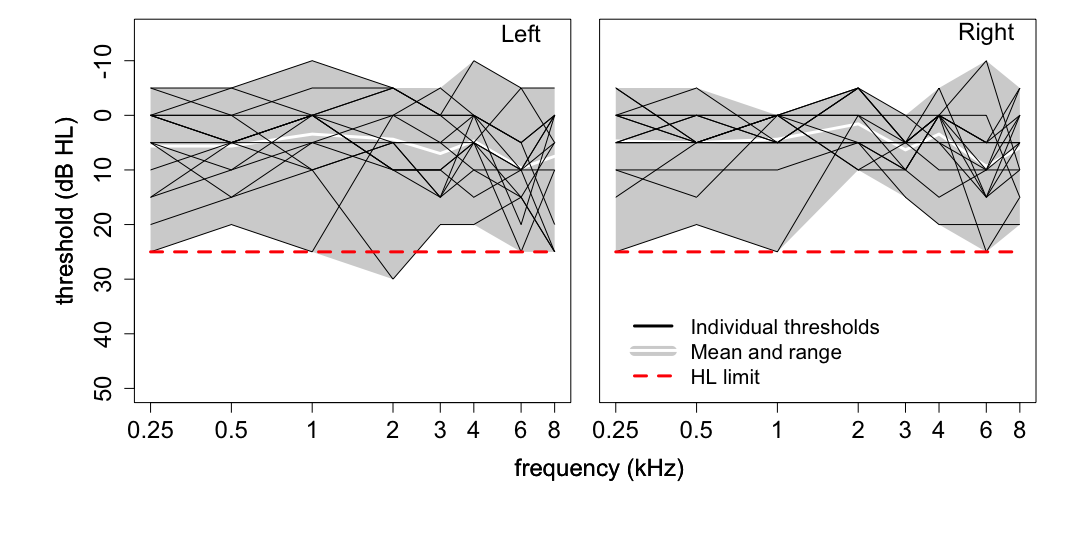
\includegraphics[width=\textwidth]{figures/Chapt1/SK_Audiogram_03042020.PNG}
%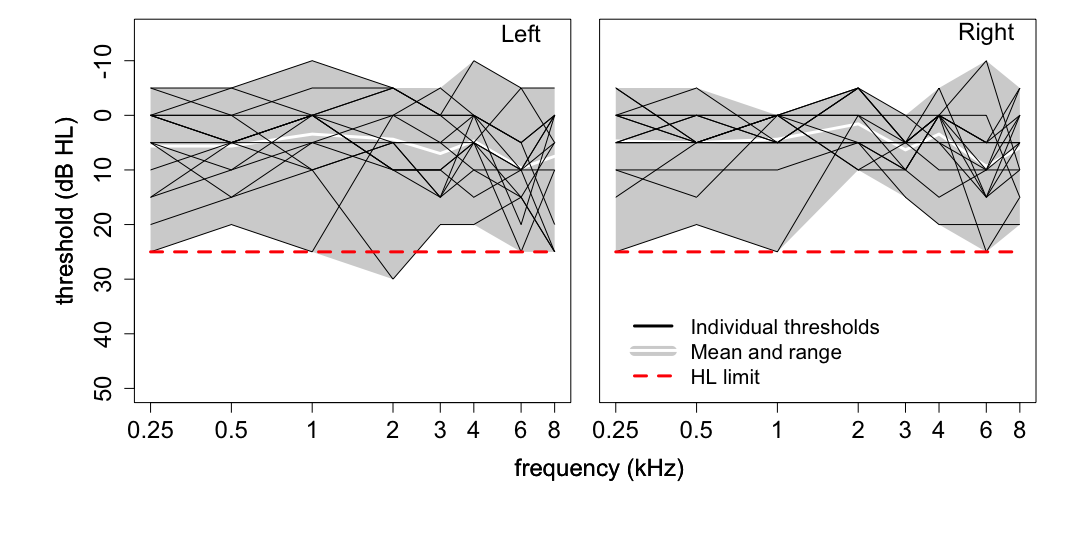
\includegraphics[scale=.45]{figures/Chapt1/SK_Audiogram_03042020.PNG}
\caption{\label{fig:PTA_Exp1}{Individual pure-tone-audiogram thresholds plotted separately for the right and the left ear (in black). The shaded grey area represents the range of the audiometric thresholds and the white line represents the mean at each frequency across the listeners. The red dashed line represents the threshold criteria of hearing level $\leq 25$ dB HL.}}
\end{figure}

\hypertarget{stimuli}{%
\paragraph{Stimuli}\label{stimuli}}

The target stimuli were taken from the Adaptive Sentence List corpus \autocite[ASL;][]{MacLeod1990}, comprising 270 sentences spoken by an adult male talker with a standard southern British English accent (sampled at 22.05~kHz with 16 bits per sample, low-pass filtered at 10~kHz). The speech material is based closely on the BKB sentences \autocite{Bench1979}, comprising simple ``everyday'' sentences of five words on average (range: 4-6 words) with three keywords each. The sentences are suitable for testing listeners with a wide range of speech perception abilities from children to adults. A loose keyword scoring method was used, whereby errors of case or declension were considered as correct responses. For example, as in a repetition of the keywords `\(<\)clown\textbf{s}\(>\) \(<\)funny\(>\) \(<\)face\textbf{s}\(>\)' to the stimulus `The \(<\)clown\(>\) had a \(<\)funny\(>\) \(<\)face\(>\)'. Six different distractors were used in the first experiment and can be grouped into two types: speech- and non-speech distractors, with different degrees of acoustic similarity to speech. The speech distractors consisted of two short unrelated conversational passages (each 5-6 sentences long) with durations roughly ranging between 15 to 30~s. They were taken from a large corpus of passages spoken by native speakers of Southern standard British English \autocite[EUROM corpus;][]{Chan1995}. Out of the two selected passages, one was spoken by a male talker, i.e., a talker of the same sex as the target talker (ENG\(_{same-sex}\)), while the second passage was spoken by a female talker (ENG\(_{opposite-sex}\)). The male talker used for the same-sex distractor was different from the one used for the target sentences. However they had similar speech rate and fundamental frequency.\\

The non-speech distractors were derived from the original speech distractors, separately for same- and opposite-sex talker, and varied in their amount of ``speech-like'' characteristics from high to low, respectively. The first one is thought to preserve the original speech temporal fine structure (TFS) associated with the speech periodicity and aperiodicity (but not that associated with overall spectral shape), and comprised of single-band vocoded speech with natural mix of periodicity and aperiodicity \autocite[FxNx; also described in][]{Steinmetzger2015}. The second non-speech distractor was an amplitude modulated speech-shaped-noise, with the same long-term spectrum, and modulation envelope as the speech distractors (AMSSN), preserving the original speech slowly varying wide-band amplitude envelope. Exemplary waveforms and spectrograms of the different distractor types are shown in Fig.~\ref{fig:MaskerType}. The distractors were generated in MATLAB (Version R2017b, Mathworks, Natick, Massachusetts) using a channel vocoder \autocites[described in][]{Green2013,Steinmetzger2015}. First, the speech distractors were bandpass filtered into a single band using zero-phase-shift 6th-order Butterworth filter (frequency range: 70 Hz - 10 kHz). The amplitude envelope was then extracted by applying full-wave rectification of the filter output and a low-pass filtering at 30 Hz (zero-phase shift, 8th-order Butterworth filter) to remove any modulations arising from voice fundamental frequency. For the generation of the AMSSN, the envelope of the single channel was multiplied with a wide-band noise carrier and the resulting waveform was low-pass filtered at 10 kHz using 6th-order elliptic filter. Next, the output signal was scaled to the RMS level of the original speech signal. FxNx was generated by multiplication of the single-band envelope with either a white noise carrier for unvoiced speech segments in the original speech, or with the fundamental frequency contour of the original signal when speech was voiced. F0 contours were extracted in PRAAT \autocite[Version 6.0.19;][]{Boersma2001} using ProsodyPro \autocite[Version 5.7.2;][]{Xu2013}, and subsequently manually corrected. Next, F0 contours were sampled at 1 kHz and interpolated through periods of voiceless and silent segments using piecewise cubic Hermite interpolation in logarithmic frequency. The start and end of each pitch contour were anchored to the signal's median frequency, resulting in a carrier with the same length as the original signal. Finally, filtering was applied to the vocoded AMSSN and FxNx signals to have the same LTASS as the original speech signals.\\

\begin{figure}[ht]
\center
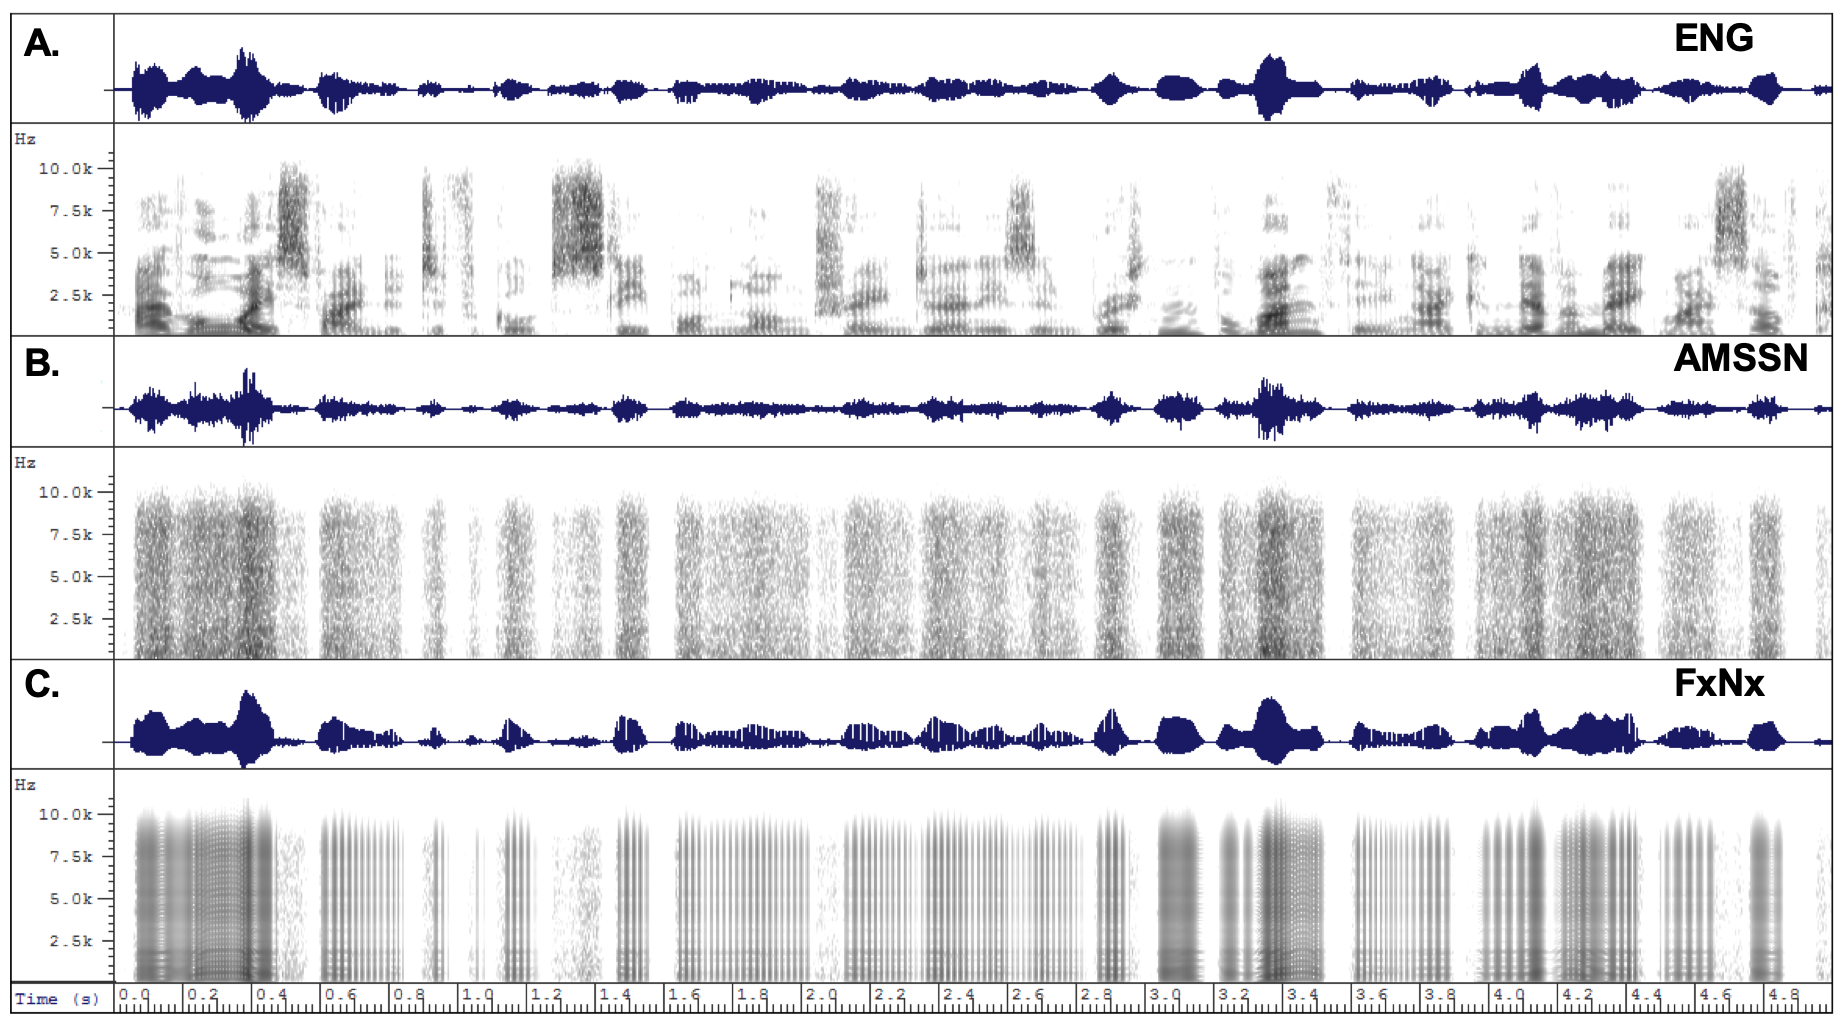
\includegraphics[width=\textwidth]{figures/Chapt1/MaskerType.PNG}
\caption{\label{fig:MaskerType}{Waveforms and broadband spectrograms of a short segment of the speech distractor spoken by a female talker, ENG$_{opposite-sex}$ (A.), and the two non-speech distractors, generated from features extracted from the original speech distractors: amplitude modulated speech spectrum noise, AMSSN (B.), and single-band vocoded speech with natural mix of periodicity and aperiodicity, FxNx (C.).}}
\end{figure}

\hypertarget{the-switching-task}{%
\paragraph{The switching task}\label{the-switching-task}}

The listening task was developed locally in MATLAB, and involves perception of target speech which is interrupted and alternated between the ears out-of-phase with an interrupted distractor, resulting in alternated segments of both signals between the two ears, with only one stimulus present in each ear at any given time.
Interruption is applied by gating the signal at a fixed modulation rate of 5 Hz, i.e., a period of 200~ms (with 5~ms rise/fall times), and varying the duty-cycle (DC), which is the proportion of time the signal is present in each modulation period. As illustrated in Fig.~\ref{fig:Interrupted}, DC ranged between 0.1, where signal is nearly completely `off' (left figures), to 0.9, where the signal is almost entirely `on' (right figures).

\begin{figure}[ht]
\center
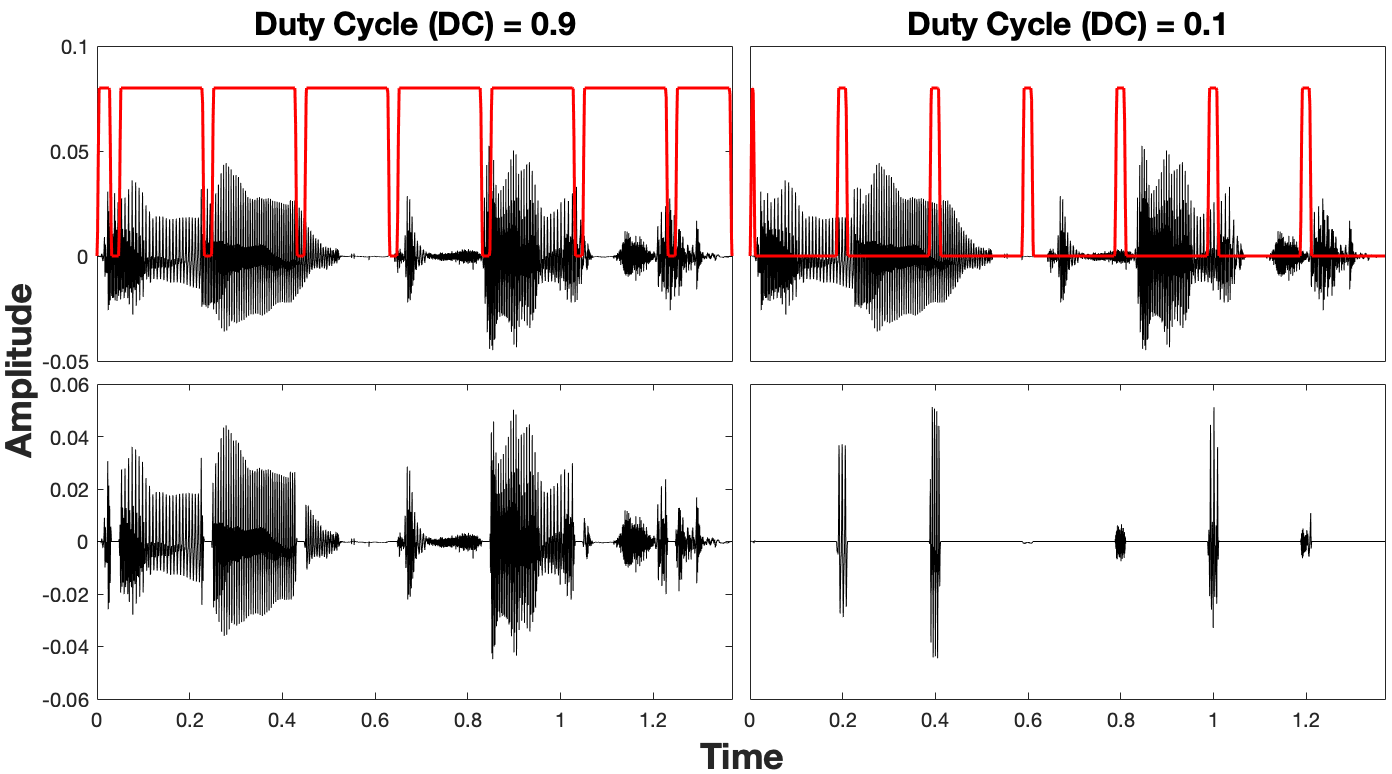
\includegraphics[width=\textwidth]{figures/Chapt1/InterruptionsExample_2020.PNG}
\caption{\label{fig:Interrupted}{Illustration of interrupted speech with varying amount of duty-cycle (DC). Upper figures: original speech signal (black) and modulation envelope (red). Bottom figures: interrupted speech following multiplication with the modulation envelope.}}
\end{figure}

Performance was estimated using a 1-up/1-down adaptive staircase procedure \autocite[e.g.,][]{Levitt1971}, whereby the speech level or signal-to-noise-ratio (SNR) is fixed, while DC varies depending on the listener's response on a trial by trial basis. The Speech Reception duty-cycle Threshold (SRdT) was estimated, which is the DC ratio at which 50\% of the keywords were repeated correctly. A correct repetition of 50\% or more of the keywords (i.e., two keywords or more), meant that the DC ratio of the next trial decreased (i.e., got more difficult), whereas a correct repetition of less than 50\% of the keywords (i.e., up to one keyword), meant that the DC ratio of the next trial increased (i.e., got easier). The points at which the specified DC changes direction are called transition reversals. The outcome measure, SRdT, is then determined by averaging the test reversals that followed three practice reversals. In case of an odd number of test reversals, the first test reversal was ignored.\\

Next, the switching of the interrupted stimuli was applied. As illustrated in Fig.~\ref{fig:Alternated}, the interrupted target signal was multiplied with a modulation carrier (grey carrier), separately for the left (blue) and the right ear (red). The modulation carrier in one of the ears was time-shifted, resulting in alternated segments of the signal between the two ears, but only in one ear at each given time (middle figures). The same step was also applied to the distractor, by inverting the modulation carriers used for the target signal. For presentation of the target speech in quiet, the distractor's segments were replaced with silence. The carrier had a fixed modulation rate of 5~Hz, which was found in several studies to significantly impair speech perception in adults and was shown to be slow enough to be able to perceive the switched speech segments between the two ears \autocite{Cherry1954}.\\

\begin{figure}[ht]
\center
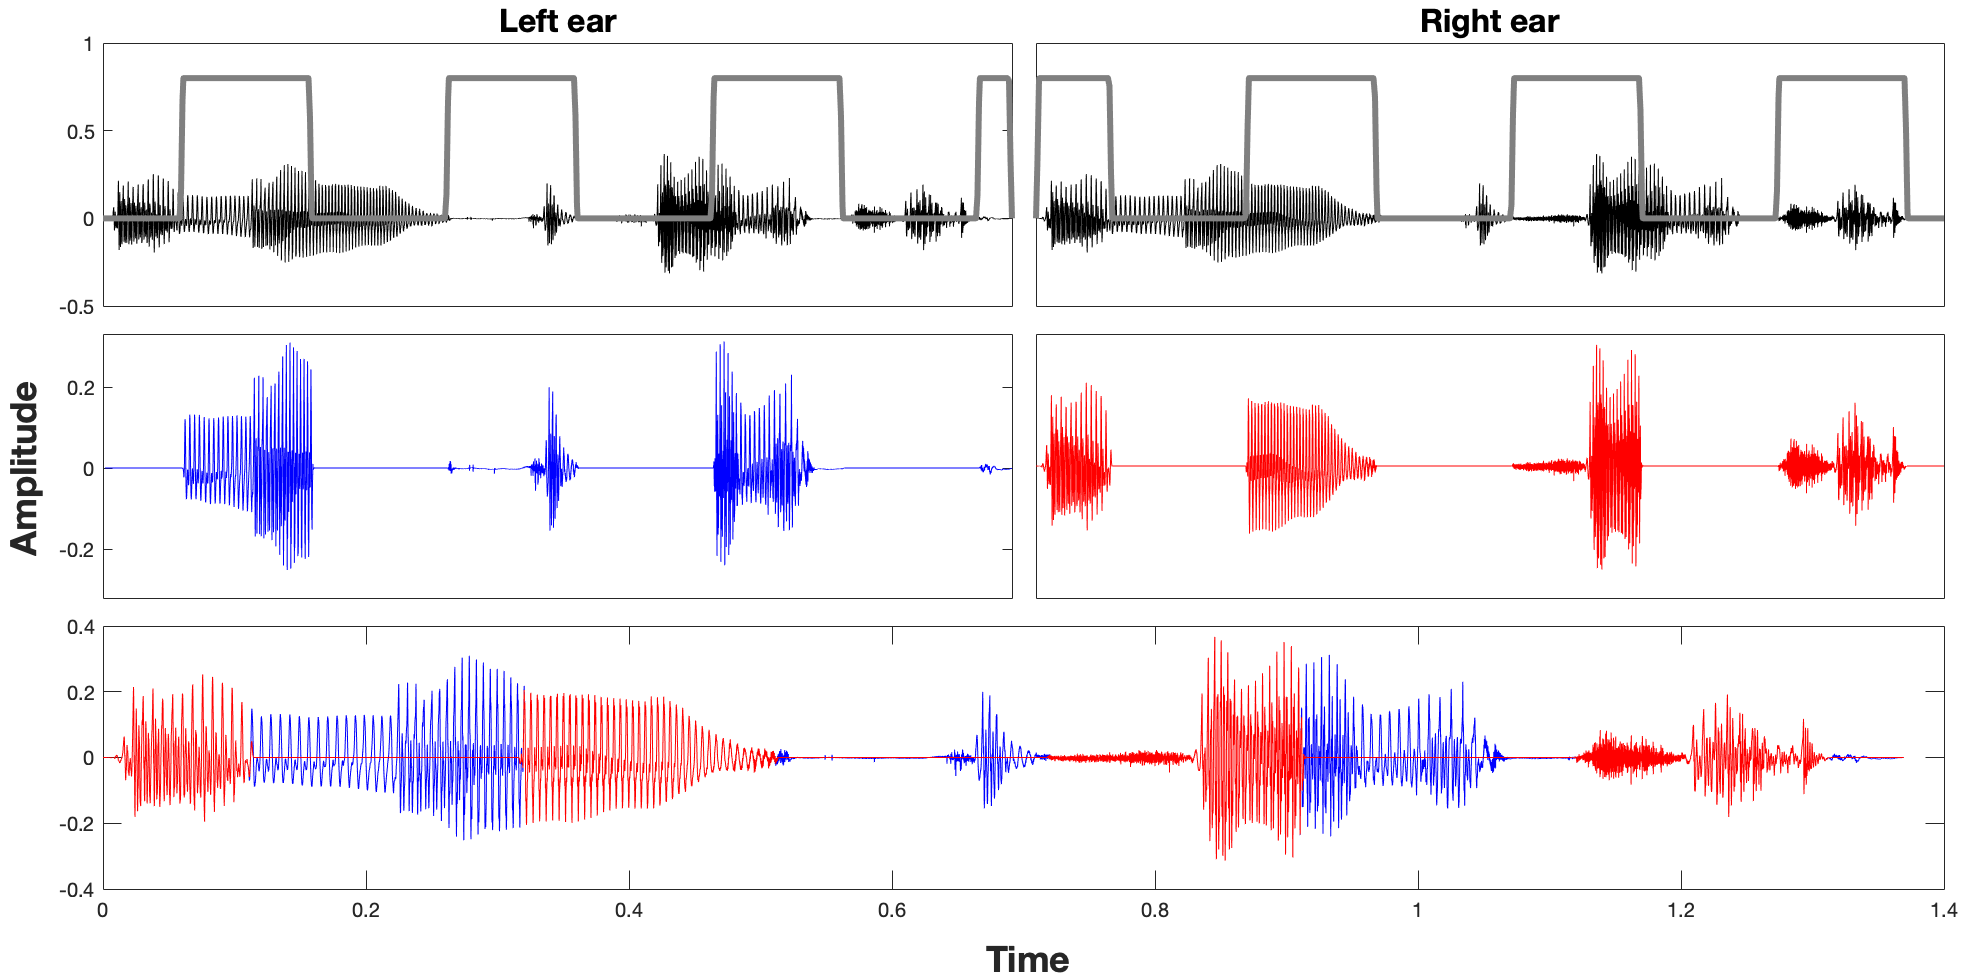
\includegraphics[width=\textwidth]{figures/Chapt1/AlternatedExample_ST.PNG}
\caption{\label{fig:Alternated}{Illustration of an alternated speech signal with a duty-cycle (DC) of 0.5 and a modulation rate of 5 Hz (i.e., 200 ms periods). Upper and middle figures shows multiplication of a modulation carrier (grey) for the left (blue) and the right (red) ear. Note that the phase of the modulation envelope is selected by random in each trial. The lower figure illustrates the alternated speech signal, achieved by adding together the left and the right channels.}}
\end{figure}

Listeners were presented with two listening conditions, with or without a distractor (see Fig.~\ref{fig:ST_ListeningConditions}). A listening condition with a distractor is depicted in the right side of the figure, where segments of interrupted target signal (black bars) and segments of the distractor signal (grey bars) are alternated out-of-phase between the left and the right ear. Similarly, a reference condition where the target signal is presented without a distractor is shown in the left half of the figure, by replacing the distractor segments with silence.\\

\begin{figure}[ht]
\center
%\centering
%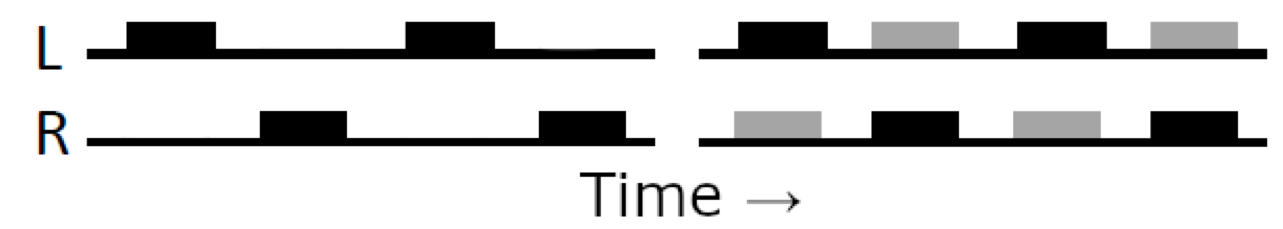
\includegraphics[width=\textwidth]{figures/Chapt1/ST_conditions.PNG}
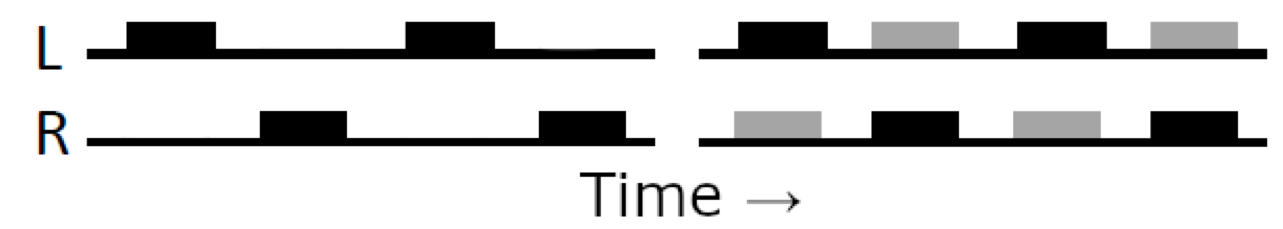
\includegraphics[scale=.5]{figures/Chapt1/ST_conditions.PNG}
\caption{\label{fig:ST_ListeningConditions}{Schematic of the switching task listening conditions. The target speech and the distractor are represented by the black and grey bars, respectively. The stimuli presented in the left ear are depicted in the upper part of the figure as a function of time, whereas the stimuli presented in the right ear are depicted in the lower part.}}
\end{figure}

\hypertarget{procedure}{%
\paragraph{Procedure}\label{procedure}}

A single experimental session with a maximal duration of 2 hours (including breaks) took place in a sound attenuated chamber. Stimulus presentation and scoring were carried out using a locally developed MATLAB script via a MacBook Pro 13 laptop (macOS High Sierra 10.13.4) connected via USB to an RME Babyface soundcard (Audio AG, Haimhausen, Germany). The test signals were presented through Sennheiser HD-25 headphones (Wedemark, Germany) at a fixed output level of circa 70 dB~SPL, measured using an artificial ear (Br"\{u\}el \& Kjær 4153, Sound and Vibration Measurements A/S, Nærum, Denmark) over a frequency range of 100 Hz to 10 kHz. A 30~ms long cosine onset ramp was applied to the segmented target signal to avoid the stimulus from sounding abrupt. For conditions with a distractor, the target onset was 1~s after the distractor to avoid uncertainty to which signal the listener should attend to. In each trial, a distractor segment was randomly selected from the long signal to match the length of the target sentence (plus 1~s onset time). The starting DC was 0.97 (i.e., signal is almost entirely present). Subsequently, the DC varied depending on the listeners response, with an initial step-size of 0.12 which decreased gradually over the first three (practice) reversals to 0.05. Nonetheless, examination of pilot data suggested that the psychometric functions of speech distractors are shallower, thus it was decided to set the minimum DC step-size speech distractors to 0.1. The starting ear of the switched segments was randomised in each trial.\\

In experiment I, a self-scoring method was used via a graphical user interface (GUI), whereby the listeners were instructed to transcribe the sentence using a keyboard and press the `OK' button once completed using a computer mouse. The response was thereafter recorded and could not be altered any more. Next, the listeners were asked to select the correctly recalled keywords from the options shown on the screen, based on their displayed transcription. Pressing again the `OK' button prompted the presentation of the next trial. Feedback was given following each trial only for the practice phase where both the non-degraded target sentence and the test stimuli were presented.
Prior to the beginning of the data collection, listeners were familiarised with the task by responding to a set of five practice runs in the following fixed order: Quiet, AMSSN, FxNx with 5 trials each, and ENG (same- and opposite-sex) with 15 trials each. The presentation order was set to reflect the expected decline in listeners' score caused by increased masking interference. Due to the limited number of ASL sentences, the target sentences in the training phase were taken from the BKB corpus \autocite{Bench1979} which are very similar in structure to the ASL sentences. In addition, a short practice run was given during the testing phase at the beginning of each run, whereas no feedback was given in order to reduce testing time.\\

In total, seven test conditions were recorded in the testing phase, originating from the following factorial design: 3 distractor types (ENG, FxNx, AMSSN) x 2 distractor talker-sex (same-/opposite-sex), and a reference condition, where the interrupted target signal was presented without a distractor (Quiet). Listeners were presented only once with each test condition. Each condition consisted of 19 ASL target sentences. The order of the test conditions and target sentence lists was quasi-randomised to account for order or fatigue effects.\\

\hypertarget{Exp1-Stats}{%
\paragraph{Statistical methods}\label{Exp1-Stats}}

\hfill\break
The listeners SRdTs was assessed using a model comparison approach in \emph{R} environment \autocite{RStudio}. Linear mixed-effects regression models (LMEMs) were fitted by maximum likelihood (ML) using the \textit{lmer()} function \autocite[\textit{lme4} package in][]{Bates2014}. The first model examined the overall effect of distractor type using 1x7 LMEM with the seven test conditions as fixed factors (3 distractor types x 2 distractor talker-sex configuration and Quiet condition), with the Quiet condition set as a reference level, and subjects included as by-subject random intercept. The second model assessed differences in performance between speech and nonspeech distractors and the effect of talker-sex using 3x2 LMEM with distractor type (ENG, FxNx, \& AMSSN) and distractor talker-sex (same/opposite) as fixed factors and again random intercepts for subjects (reference levels: distractor type = AMSSN; distractor talker-sex = opposite). Note that observations for the Quiet condition were excluded from the second model. LMEM assumptions of homogeneity and normal distribution were fulfilled, tested with Levene's test \autocite{Car_LevenTestRPackage} and Shapiro-Wilk test \autocite{Stats_ShapiroWilkRPackage}. The initial saturated model included by-subject random intercepts and slopes. However, because the model did not converge, it was simplified to a model that would converge by including only random intercepts. We used backward model selection \autocite[cf.][]{Barr2013}, by removing fixed terms that did not significantly degrade the model's fit (significance level \(\alpha =0.05\)) using likelihood ratio test (\(\chi^2\)). Independent post-hoc t-test comparison was performed on the fitted model and included adjusted least-squared-mean for the random intercepts (subjects) using \textit{lsmeans()} \autocite[lsmeans package;][]{Lenth2016}. The p-values were Bonferroni-adjusted.\\

\hypertarget{results}{%
\subsubsection{Results}\label{results}}

Descriptive statistics of the listeners performance (in SRdTs) for the different test conditions is given in Tab.~\ref{tab:Exp1_Discriptive}. In total, seven SRdTs were recorded for each participant across four background conditions: Quiet, and the distractors AMSSN, FxNx, and ENG, whereby distractors originated from either opposite- or same-sex talker. Boxplots of the SRdTs are shown in Fig.~\ref{fig:Exp1BoxPlot}. The results reveal that the non-speech distractors elicited little to no interference with the target speech, with similar SRdTs as for the reference Quiet condition, while the speech distractors showed a large interference effect, resulting in increased SRdTs (i.e., poorer performance) for opposite-sex and same-sex talkers.\\

To put these results in what might be a more understandable context, the SRdT reflects the amount of speech information (glimpses) required by the listeners to understand 50\% of the sentence correctly. An SRdT of roughly 0.34 obtained for the non-speech distractors and the reference condition Quiet (at a 5~Hz modulation rate) is equivalent to five 68~ms audible glimpses of the target sentence per second, each preceded and followed by 132~ms of silence. For the speech distractors on the other hand, in order to understand 50\% of the sentence correctly, the listeners needed more than double the duration of audible target glimpses per period (164~ms) for the same-sex distractor and about 56\% longer (106~ms) for the opposite-sex distractor.\\

The effect of distractor type in general on the listeners' performance, was tested by a comparison of the SRdTs with the reference (Quiet) condition included using 1x7 LMEM (see Tab.~\ref{tab:Exp1_LMEM} for the model coefficients and p-values). Model comparison showed a highly significant main effect of background {[}\(\chi^{2}\)(6)=178.76, \(p\) \textless 0.001{]}. The results revealed that speech distractors significantly impaired the listeners performance, for both opposite- and same-sex talker {[}b=0.19, t(96)=7.08, \(p\) \textless 0.001 and b=0.48, t(96)=17.66, \(p\) \textless 0.001, respectively{]}. On the other hand, no difference in performance between the non-speech distractors (AMSSN \& FxNx) and the reference condition was found (all \(p's\) \textless 0.05).~

\begin{table}[ht]
\center
\caption{Descriptive statistics for the SRdTs obtained in experiment I across the different test conditions.}
\label{tab:Exp1_Discriptive}
\renewcommand{\arraystretch}{2}
\begin{tabular}{lccc}
\hline \hline
 &  & \multicolumn{2}{c}{Distractor talker-sex} \\ \cline{3-4} 
Background type & \begin{tabular}[c]{@{}c@{}}Grand mean\\ M (SD)\end{tabular} & \begin{tabular}[c]{@{}c@{}}Opposite\\ M (SD)\end{tabular} & \begin{tabular}[c]{@{}c@{}}Same\\ M (SD)\end{tabular} \\ \hline
Quiet & 0.34 (0.07) & - & - \\
AMSSN & 0.35 (0.09) & 0.34 (0.08) & 0.35 (0.09) \\
FxNx & 0.37 (0.09) & 0.37 (0.08) & 0.36 (0.10) \\
ENG & 0.67 (0.18) & 0.53 (0.13) & 0.82 (0.09) \\ \hline \hline
\\
\end{tabular}
\end{table}

\begin{table}[ht]
\center
\caption{\label{tab:Exp1_LMEM}{1x7 mixed-effects model for SRdTs measured in experiment I across all subjects (N observations $=$ 112; N Subjects $=$ 16). Reference level = Quiet condition. Significant p-values are marked as bold.}}
\renewcommand{\arraystretch}{2}
\begin{tabular}{lccc}
\hline \hline
\multicolumn{4}{l}{SRdT $\sim$ BackgroundType + (1 $\mid$ Subjects)}                               \\ \hline
Main effects           & Df                        & $\chi^2$ & $p$                                  \\ \hline
BackgroundType         & 6                         & 178.76   & \textbf{$<$0.001} \\ \hline
Fixed effects          & Estimated mean difference & SE       & 95 \% CI                           \\ \hline
intercept              & 0.34                      & 0.02     & 0.29 – 0.38                        \\
AMSSN$_{opposite-sex}$ & 0.00                      & 0.03     & -0.05 – 0.06                       \\
AMSSN$_{same-sex}$     & 0.01                      & 0.03     & -0.04 – 0.07                       \\
FxNx$_{opposite-sex}$  & 0.04                      & 0.03     & -0.02 – 0.09                       \\
FxNx$_{same-sex}$      & 0.02                      & 0.03     & -0.03 – 0.08                       \\
ENG$_{opposite-sex}$   & 0.19                      & 0.03     & 0.14 – 0.24                        \\
ENG$_{same-sex}$       & 0.48                      & 0.03     & 0.43 – 0.53                        \\ \hline \hline
%Random effects         & \multicolumn{3}{c}{Variance}                                              \\ \hline
%Subjects (intercept)   & \multicolumn{3}{c}{0.002}                                                 \\
%Residual               & \multicolumn{3}{c}{0.006}                                                 \\ \hline \hline  
\\
\end{tabular}
\end{table}

\begin{figure}[ht]
\center
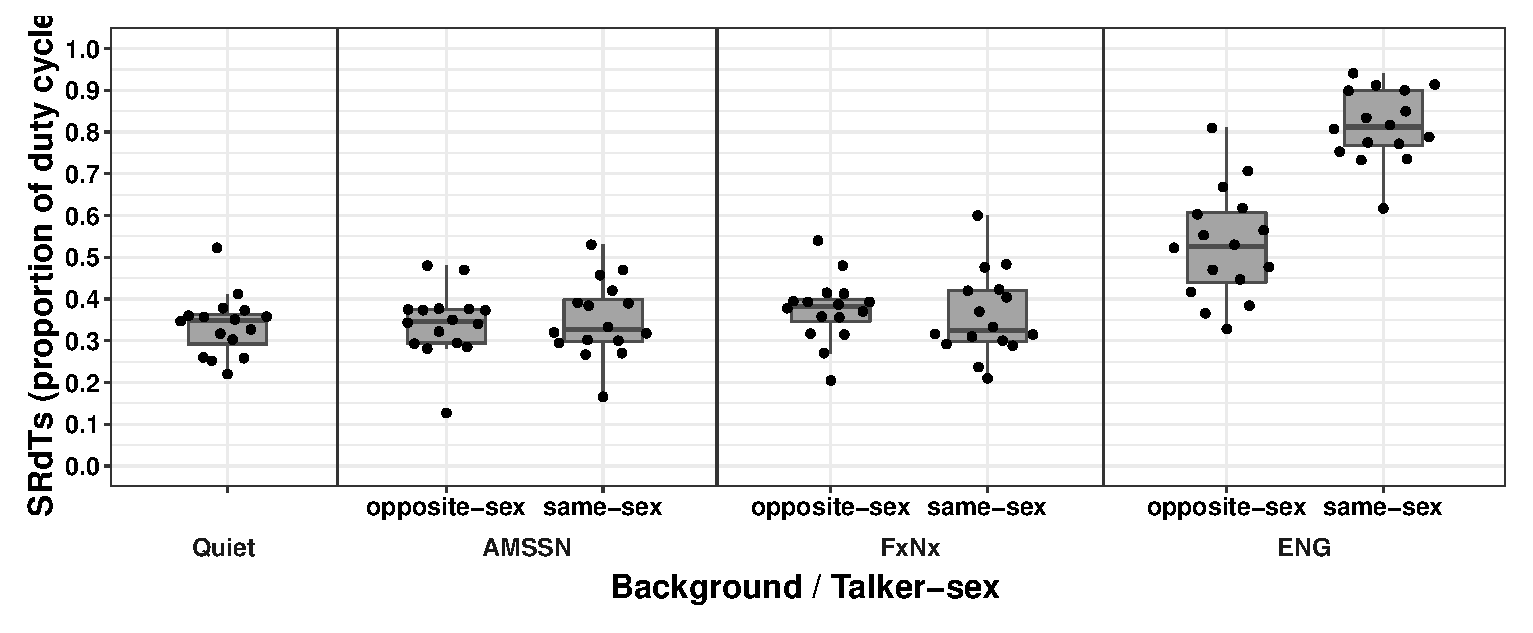
\includegraphics[width=\textwidth]{figures/Chapt1/dcBoxplot_Exp1_2020-04-06.eps}
%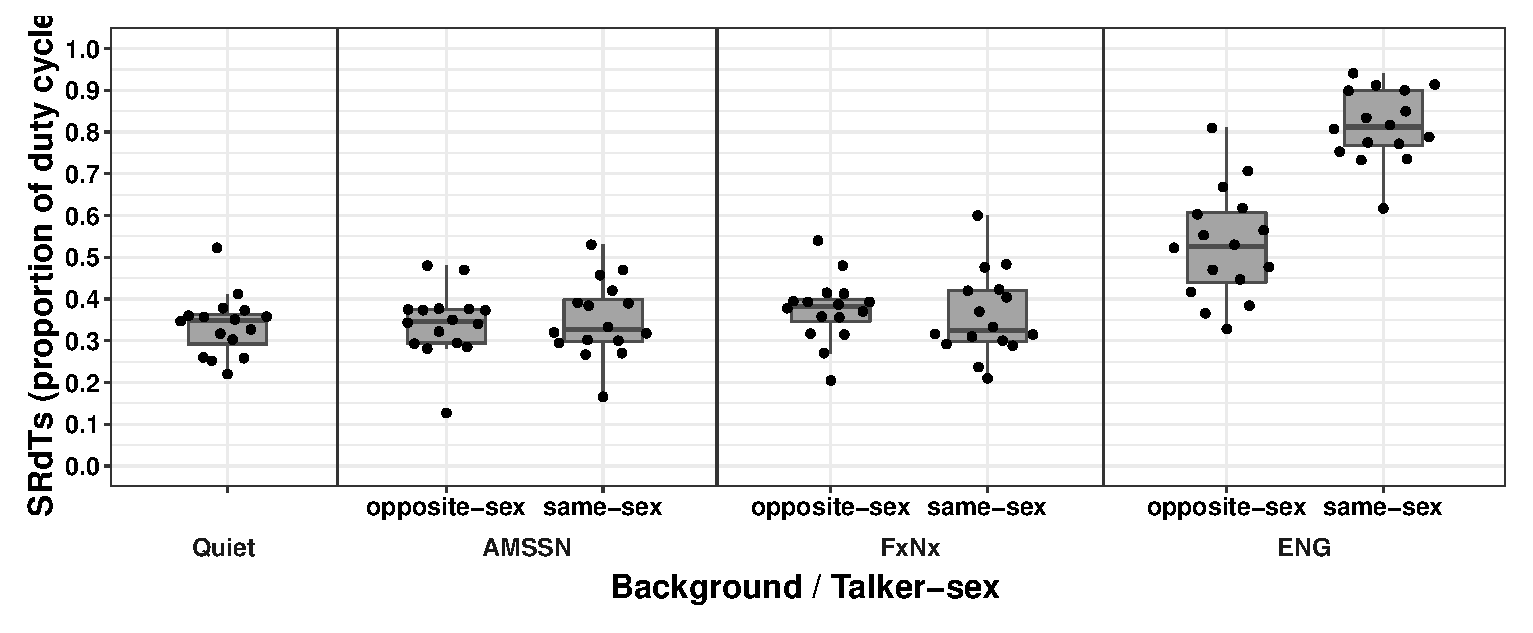
\includegraphics[scale=.65]{figures/Chapt1/dcBoxplot_Exp1_2020-04-06.eps}
\caption{\label{fig:Exp1BoxPlot}{Boxplots of the SRTds measured in experiment 1 for the baseline condition Quiet and the distractor conditions AMSSN, FxNx and ENG with the same- and opposit-sex talker. Individual scores are represented by the black circles.}}
\end{figure}

A separate model without observations measured with the Quiet condition examined whether there was a difference in performance between the speech and nonspeech distractors, \textbf{as well as the effect of distractor talker-sex} using 3x2 LMEM (see Tab.~\ref{tab:Exp1_LMEM2}). Model comparison showed a significant main effect for distractor type {[}\(\chi^{2}\)(5)=159.45, \(p\) \textless 0.001{]}, distractor talker-sex {[}\(\chi^{2}\)(3)=72.08, \(p\) \textless 0.001{]} and their interaction {[}\(\chi^{2}\)(2)=54.96, \(p\) \textless 0.001{]}.
Next a post-hoc t-test comparison showed no significant difference in SRdTs between the two non-speech distractors FxNx and AMSSN {[}t(85.33)=1.11, \(p=0.808\){]}, and a highly significant difference between the non-speech and speech distractors {[}AMSSN vs.~ENG: t(85.3)=-16.85; FxNx vs.~ENG: t(85.3)=-15.73, \(p<0.001\){]} . Moreover, differences in performance due to distractor talker-sex (two-way interaction) was significant (and highly so) only for the speech distractors {[}t(85.3)=-10.46, \(p<0.0001\){]}.\\

\begin{table}[ht]
\caption{\label{tab:Exp1_LMEM2}{3x2 mixed-effects model for SRdTs measured in experiment I across all subjects (N observations $=$ 96; N Subjects $=$ 16. Reference levels: distractor type = AMSSN; distractor talker-sex = opposite. Significant p-values are marked as bold.}}
\renewcommand{\arraystretch}{2}
\begin{tabular}{lccc}
\hline \hline
\multicolumn{4}{l}{SRdT $\sim$ DistrType  + DistrTlkrSex + DistrType $\ast$ DistrTlkrSex + (1 $\mid$ Subjects)}                                \\ \hline
Main effects                                                                        & Df                        & $\chi^2$ & $p$          \\ \hline
DistrType                                                                           & 5                         & 159.45   & \textbf{$<$0.001}        \\
DistrTlkrSex                                                                        & 3                         & 72.08    & \textbf{$<$0.001}        \\
DistrType x DistrTlkrSex                                                            & 2                         & 54.96    & \textbf{$<$0.001}        \\ \hline
Fixed effects                                                                       & Estimated mean difference & SE       & 95 \% CI     \\ \hline
intercept                                                                           & 0.34                      & 0.02     & 0.30 – 0.39  \\
DistrType  (FxNx)                                                                   & 0.03                      & 0.03     & -0.02 – 0.08 \\
DistrType  (ENG)                                                                    & 0.19                      & 0.03     & 0.14 – 0.24  \\
DistrTlkrSex (same)                                                               & 0.01                      & 0.03     & -0.04 – 0.06 \\
\begin{tabular}[c]{@{}l@{}}DistrType (FxNx) x\\ DistrTlkrSex (same)\end{tabular} & -0.02                     & 0.04     & -0.10 – 0.05 \\
\begin{tabular}[c]{@{}l@{}}DistrType (ENG) x\\ DistrTlkrSex (same)\end{tabular}  & 0.28                      & 0.04     & 0.20 – 0.35  \\ \hline \hline
%Random effects                                                                      & \multicolumn{3}{c}{Variance}                        \\ \hline
%Subjects (intercept)                                                                    & \multicolumn{3}{c}{0.003}                           \\
%Residual                                                                                       & \multicolumn{3}{c}{0.006}                           \\ \hline \hline
\\
\end{tabular}
\end{table}

\hypertarget{discussion}{%
\subsubsection{Discussion}\label{discussion}}

The objective of the first experiment was to evaluate the amount of IM induced by different types of speech and non-speech distractors with or without talker-sex agreement between the target and the distractor. To tease apart the key factors that contribute to IM, speech intelligibility was measured for three types of distractors. In addition, the listeners' baseline performance was measured for the switched target with silent intervals replacing the distractor (Quiet condition).\\

The SRdTs measured in the reference Quiet condition (0.34 \(\pm\)~0.07) is in line with Akinseye \autocite*[unpublished BSc thesis,][]{Akinseye2015} preliminary study, and is in accordance with the literature for interrupted speech \autocites[e.g.,][]{Miller1950,Kidd2012} and alternated speech \autocite[e.g.,][]{Stuart2008}. Different distractor types affect performance differently. We hypothesised that performance will get poorer (i.e., higher DC) by introducing a distractor and that the decline in speech perception (or the increase in IM) will be moderated by the type of the distractor, with speech distractors potentially producing the largest IM. Moreover, we hypothesised that introducing more speech-like features into the non-speech distractors would result in increased similarity and uncertainty between the target and the the distractor, which consequently will result in a larger interference effect for FxNx as opposed to AMSSN. We therefore expected FxNx to introduce similar IM as the speech distractor. The outcomes of the study showed that speech distractor (ENG) resulted in the largest IM. In fact, only the speech distractor showed a significant difference in performance, while performance for the non-speech distractors was the same as for the target sentences in quiet.\\

Informational masking can be attributed to both bottom-up processes, as in signal characteristics that support streaming of a sound source (i.e., object formation) and top-down attention-related processes that support attending to the target signal \autocite[i.e., object selection;][]{Shinn-Cunningham2008}. Increased target-distractor similarity and uncertainty increases IM. The present study revealed that only the speech distractor produced IM. Due to the complex nature of speech signals, trying to disentangle the different contributing factors that produced this exclusive IM effect for speech distractors is not straight forward. Although some properties of the stimuli (i.e., speech distractors and their derived nonspeech distractors) we used were to some extent controlled for, due to the variable nature of speech, some differences between the stimuli are still possible (e.g., sentence structure, semantic content, vocabulary, speech rate, vocal-tract length, F0, or generally different speaking style), and could have had an effect on the amount of IM that is produced. Nevertheless, one obvious factor that had a large effect on the amount of IM was the distractor talker-sex. Performance for speech distractors spoken by a same-sex talker was significantly poorer (i.e., larger DC) than for a distractor spoken by a talker from the opposite sex. In the present study we chose a same-sex distractor talker with a similar median F0 as the target talker. This may add an element of uncertainty with the target signal, resulting in a combination of bottom-up failure in object formation in addition to the impaired top-down object selection as seen for the opposite-sex distractor talker. Nonetheless, the stimuli used in the present study originated from single talkers and did not change from trial to trial. Thus, one should be cautious when trying to draw more general conclusions about the effect of the talker-sex agreement between the target and the distractor on the performance.\\

Another possible contributing factor is semantic content. The speech signals in the present study originated from different talkers and differed in their semantic content: ASL sentences (target) vs.~unrelated connected speech (distractor). Nonetheless, similarity between the target and speech distractors at the word-level, or more likely at the phoneme-level are short enough to be conveyed within the 200~ms long switching signal segments, and could potentially cause attentional uncertainty, resulting in failure of top-down processing in attending to the target signal. The lack of IM interference for FxNx may suggest that semantic content is weighted as a more reliable cue in the process of auditory stream segregation in adverse listening conditions (such as here), and may have been prioritised over other cues such as F0 and TFS. The unaffected performance for amplitude modulated speech shaped noise was expected and is in line with other studies demonstrating that typically neurotypical normal hearing adults can maintain high intelligibility for speech in amplitude modulated noise when presented dichotically \autocite[e.g.,][]{Brungart2013}.\\

Overall, these results suggests the important role of semantic content in IM in the switching task. However, further research should be done to investigate this more closely. One possible way to look into the contribution of meaning of the speech distractors is to include speech distractors spoken in a language that the listeners are not familiar with, thus preserving the natural spectrotemporal characteristics of speech, while eliminating the influence of semantic content.\\

The present study used an automated self-scoring method to record the listeners performance. All the participants were able to adequately use the scoring method with no particular problems. This was supported by an inspection of the listeners' transcription and selected keywords. Automated scoring methods in speech perception tasks are mostly used for closed set speech material such as the matrix sentences \autocite{Kollmeier2015} or the coordinate response measure \autocite[CRM;][]{Bolia2000}. The main advantage of the scoring method used in the current study is that it enables a fully automated testing for open set speech material. Thus, it excludes the need for the examiner to manually select the listener's verbal response and eliminates the need of the examiner to speak the language spoken in the task. Selecting the listener's correct answer based on their verbal response in some cases can introduce bias to the measurement (e.g., when the listener has pronunciation difficulties). Therefore, this method avoids such bias and has the potential to reduce the scoring error rate. Nonetheless, it has two major disadvantages which probably makes this method most likely not suitable for children and elderly listeners, nor for use in the clinic listeners or clinically viable. First, it requires adequate typing and spelling skills and working memory may possibly affect the listeners' performance, especially in adverse listening conditions. Secondly, it substantially increase the testing time, and testing times vary greatly depending on the listeners typing skills.\\

\hypertarget{experiment-ii-speech-distractors-spoken-in-a-familiar-vs.-unfamiliar-language}{%
\subsection{Experiment II: speech distractors spoken in a familiar vs.~unfamiliar language}\label{experiment-ii-speech-distractors-spoken-in-a-familiar-vs.-unfamiliar-language}}

Findings in the first experiment demonstrated that performance in the task is specifically affected when speech distractors are used, and that this IM effect did not occur for the non-speech distractors. To extend these findings, in the second experiment we examined the contributions to IM of familiarity with the spoken language of the distractor (English vs.~Mandarin), and similarity-related features as in voice characteristics of the talkers (same-sex vs.~opposite-sex talkers). Furthermore, the applicability of the proposed task for future clinical and research use was examined.\\

\hypertarget{methods-1}{%
\subsubsection{Methods}\label{methods-1}}

\hypertarget{participants-1}{%
\paragraph{Participants}\label{participants-1}}

The data in the second experiment was taken from a larger study which aimed to compare performance in the task between two groups of young and older adults, native British English speakers with 20 listeners in each group \autocite{Huang2018}. None of the participants were familiar with Mandarin. Here we present only the data collected with the younger group. To enable a better comparison of listeners scores between experiment I and II, the same inclusion criteria were employed. Thus, only listeners with an age \(\leq\)~35 years old were included, resulting in a total of 15 listeners. Next, inspecting for outliers (more than 2 s.d.'s from the mean), revealed that one listener was indicated as a possible outlier 9 times out of 10 with an over all poor performance, and was therefore removed. The remaining 14 listeners mean age was 25.1 \(\pm\) 4.2 (range: 19-35 years, 11 females) and were tested to have normal hearing acuity based on the same criteria as in the previous experiment (right ear \(PTA_{4}=3.6 \pm 2.6\) dB~HL, left ear \(PTA_{4}=4.1 \pm 3.2\) dB~HL; see Fig.~\ref{fig:PTA_Exp2}). Participants were recruited from the UCL psychology subject pool and from the Speech and Language Therapy MSc programme at City, University of London and were paid for their participation. The Study was approved by the UCL research Ethics Committee (Project ID Number 0544/006).\\

\begin{figure}[ht]
\center
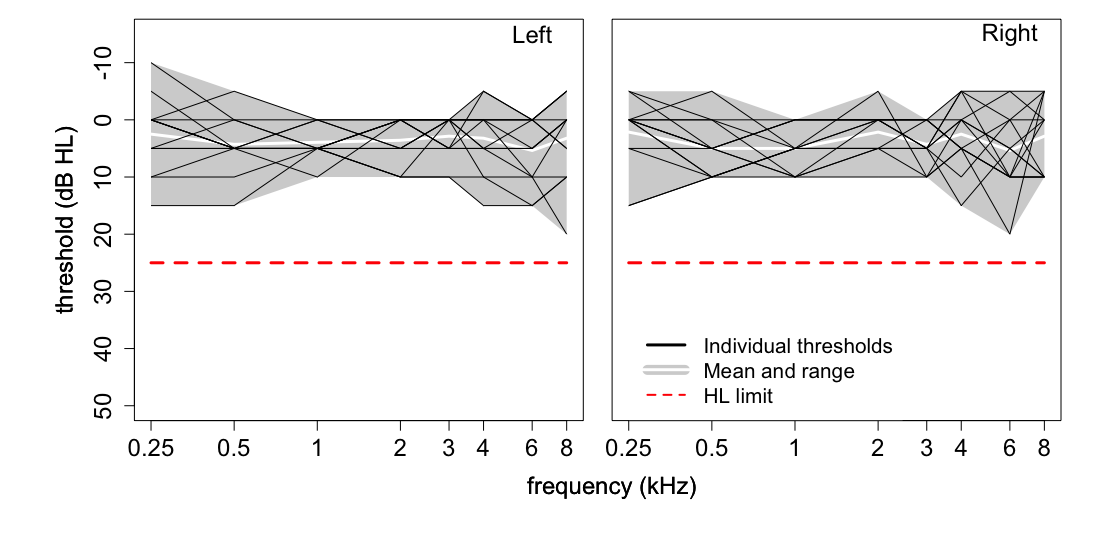
\includegraphics[width=\textwidth]{figures/Chapt1/Exp2_PTA.PNG}
\caption{\label{fig:PTA_Exp2}{Individual pure-tone-audiogram thresholds plotted separately for the right and the left ear (in black). The shaded grey area represents the range of the audiometric thresholds and the white line represents the mean at each frequency across the listeners. The dashed line represents the threshold criteria of hearing level $\leq 25$ dB HL.}}
\end{figure}

\hypertarget{stimuli-1}{%
\paragraph{Stimuli}\label{stimuli-1}}

The same ASL target sentences were used in the second experiment. Nonetheless, unlike the first experiment where the frequency range of the stimuli extended up to 10~kHz, the stimuli in the current experiment were low-pass filtered at 4~kHz. This was carried out in order to minimise the effects of any possible high-frequency hearing loss in the older-adult group, which is known to increase in prevalence with age \autocite[e.g.,][]{Brant1990}. As in the previous experiment, several speech and non-speech distractors were used. However, only data for speech distractors will be discussed here. The speech distractors in experiment II consisted of either familiar English passages (ENG), originating as before from the EUROM corpus, or unfamiliar Mandarin passages (MDR), spoken by native Mandarin Chinese adult speakers. The Mandarin passages were recorded in the Department of Speech, Hearing, and Phonetics Sciences, University College London (UCL) in an anechoic chamber and followed similar recording and editing steps as in the EUROM passages \autocite{Chan1995}. Each of the speech distractors (ENG and MDR) comprised twenty different talkers (10 same-sex and 10 opposite-sex), with a total of forty different speech passages.\\

\hypertarget{procedure-1}{%
\paragraph{Procedure}\label{procedure-1}}

A similar experimental design was employed in the second experiment with a few exceptions. Instead of a self-scoring method, listeners were asked to verbally repeat the target sentences to the experimenter who was situated alongside the participant in the sound treated chamber. The experimenter scored the response by selecting the correctly repeated keywords on the screen. Listeners were encouraged to guess if unsure and no feedback was given at any time. Additionally, while in the first experiment the same passage was used throughout the testing, here, a distractor passage was selected at random out of the ten different passages in each trial. Finally, each test condition was measured twice with no repetition of the target sentences. The order of the test conditions was pseudo-randomised.\\

\hypertarget{results-1}{%
\subsubsection{Results}\label{results-1}}

In the second experiment, listeners were presented with the target sentences without a distractor (Quiet), and with a speech distractor spoken either in a familiar or unfamiliar language (ENG and MDR, respectively) spoken by either same-sex or opposite-sex distractor talkers than the target talker. Each participant was presented with two runs for each test condition with a total of 10 runs (5 conditions x 2 runs).\\

\hypertarget{within-session-test-retest-reliability}{%
\paragraph{Within-session test-retest reliability}\label{within-session-test-retest-reliability}}

Descriptive statistics of the listeners performance (in SRdTs) for the different test conditions is given in Tab.~\ref{tab:Test-RetestDiscriptive}. A comparison between the test runs is depicted in Fig.~\ref{fig:Exp2_2runs}, with the SRdTs obtained in the first run (x-axis) plotted as a function of the second run (y-axis). The figure reveals that most observations are fairly close to or on the diagonal line across the different test conditions, which represents an identical performance between the first and the second run.\\

\begin{figure}[ht]
\center
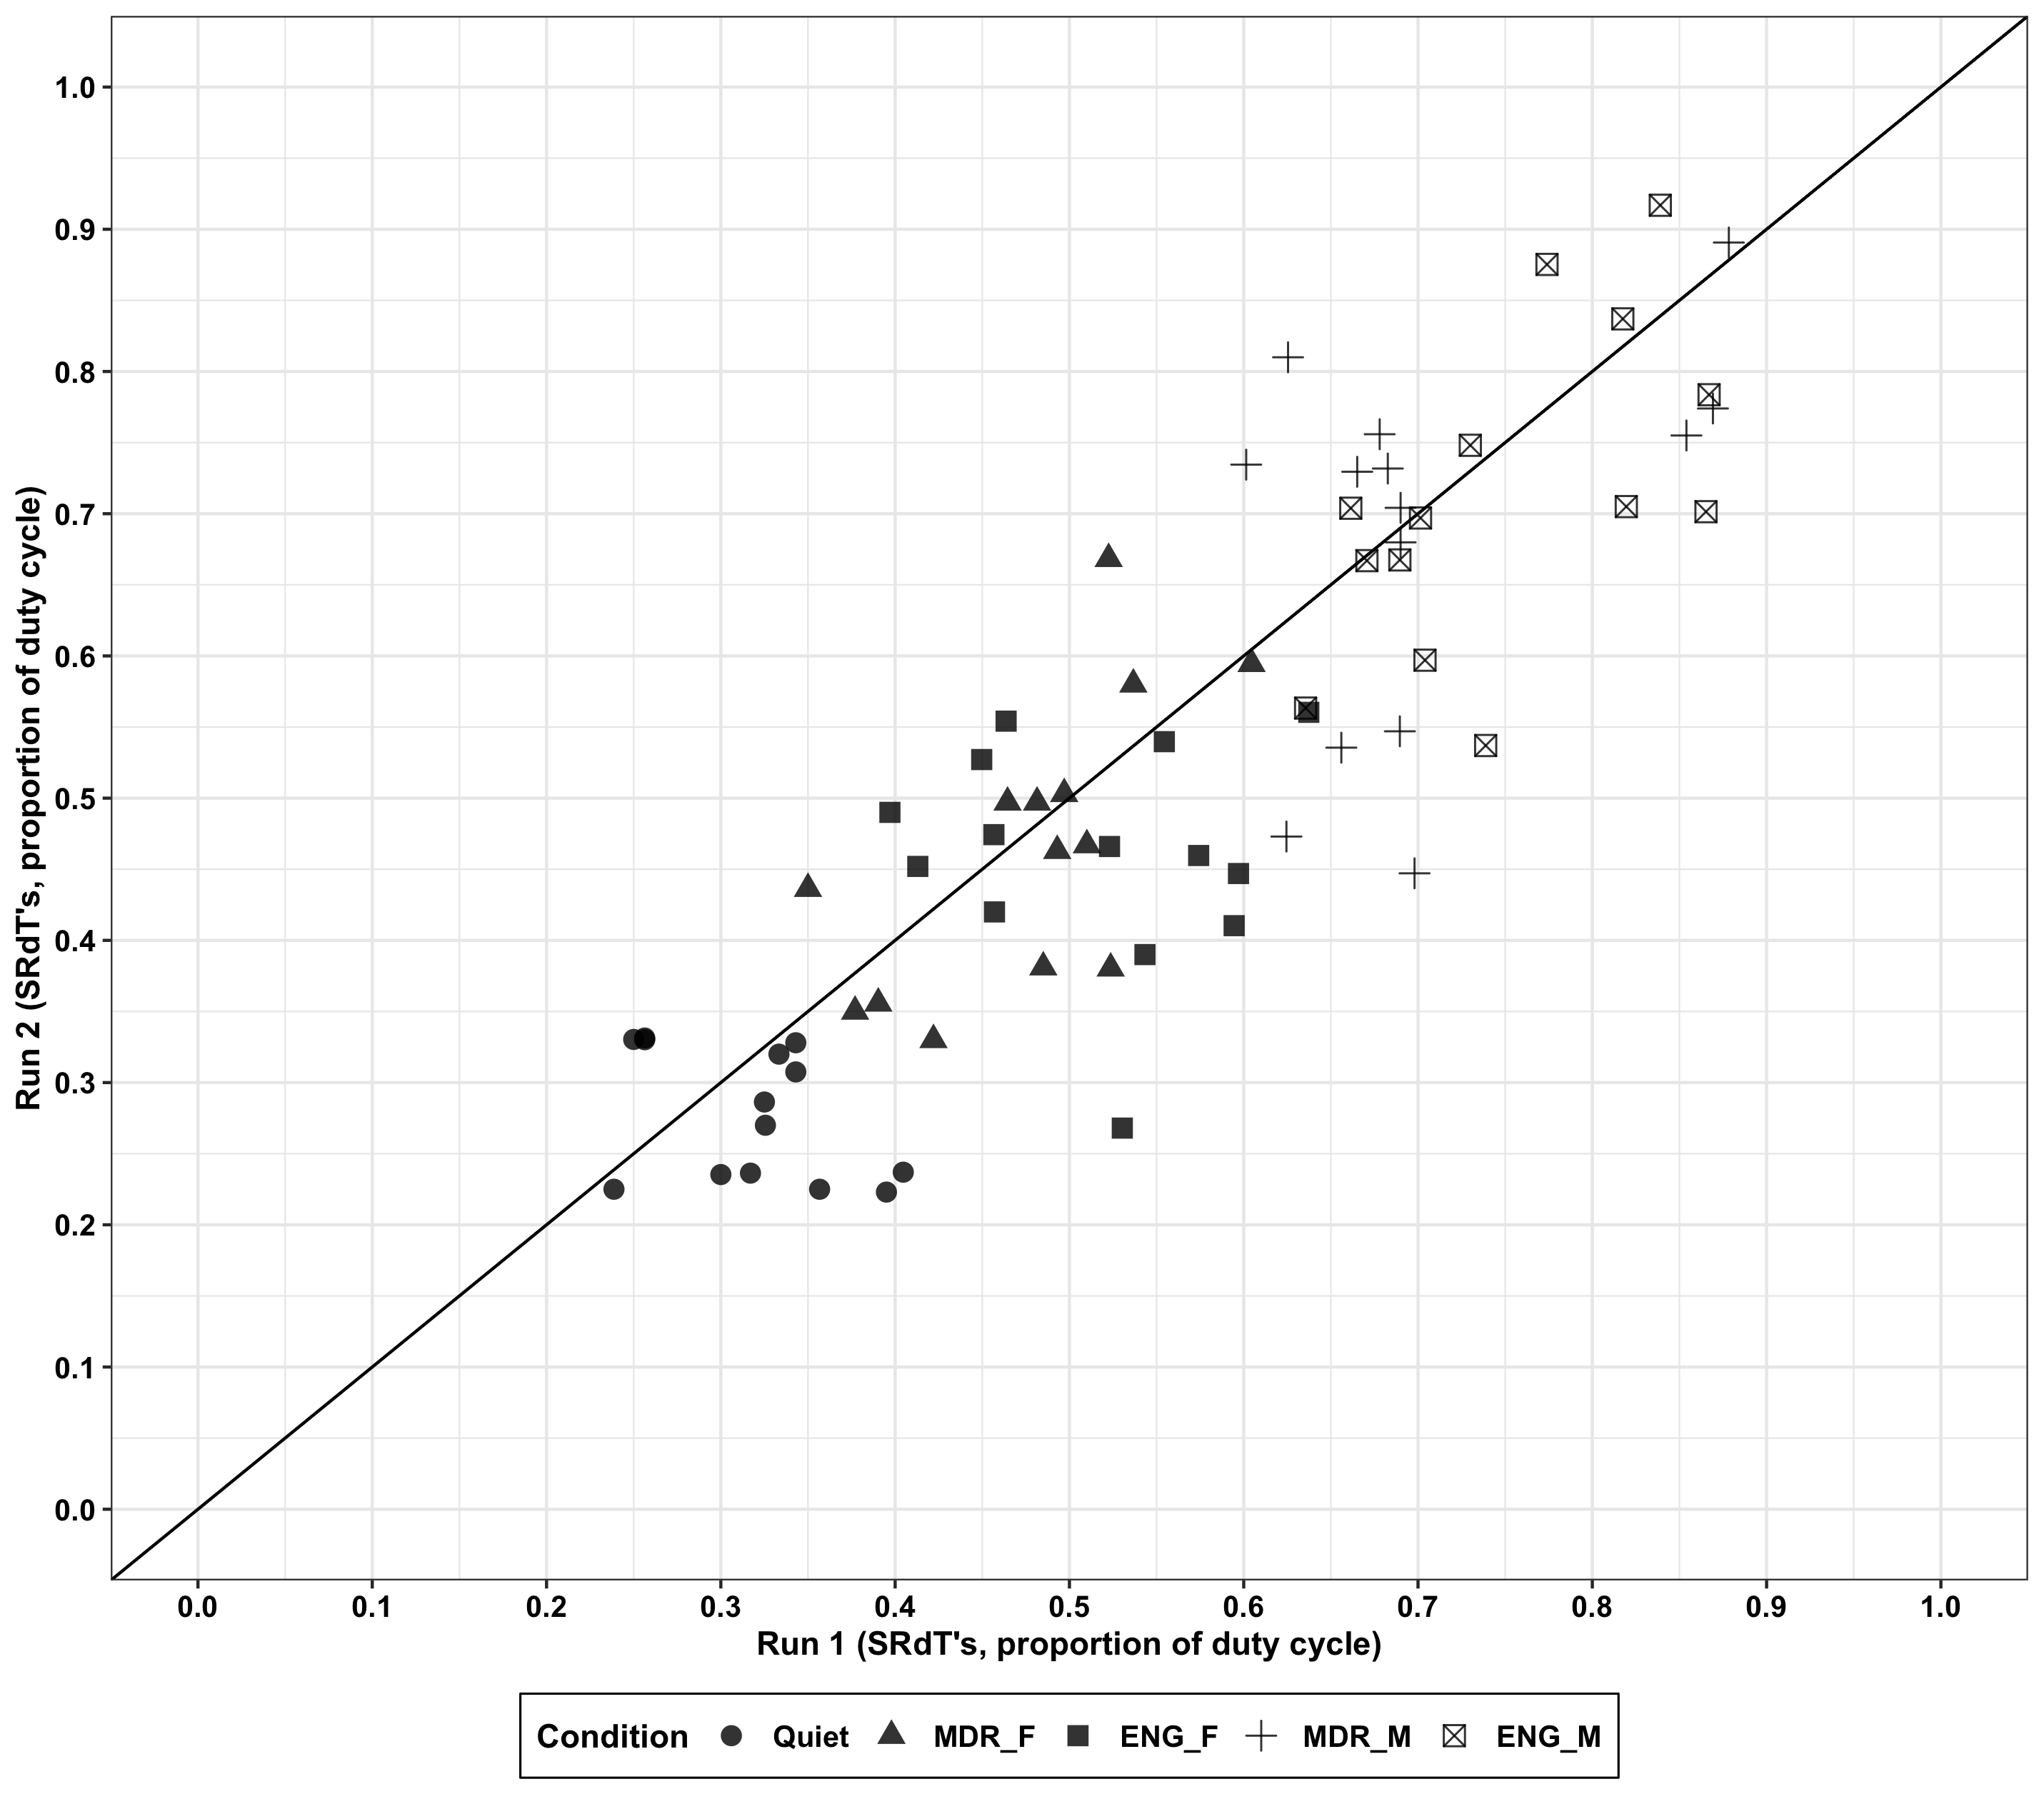
\includegraphics[width=\textwidth]{figures/Chapt1/Exp2_Run1_Run2_2021-01-29.png}
\caption{\label{fig:Exp2_2runs}{Test-retest SRdTs obtained in experiment II for the test conditions Quiet, ENG$_{opposite-sex}$ and ENG$_{same-sex}$. Individual scores are represented by the different shapes corresponding to the test condition, whereby the diagonal line represents an optimal agreement between run 1 and 2.}}
\end{figure} 

\begin{table}[ht]
\caption{\label{tab:Test-RetestDiscriptive}{Descriptive statistics for SRdTs obtained in experiment II with M indicates the mean and SD for the listeners SRdTs, whereas the grand mean indicates the aggregated data across both experiments.}}
\renewcommand{\arraystretch}{2}
\begin{tabular}{lcccccc}
\hline \hline
                & \multicolumn{6}{c}{Distractor talker-sex}                                                      \\
                & \multicolumn{3}{c}{Opposite M (SD)}            & \multicolumn{3}{c}{Same M (SD)}                    \\ \cline{2-7} 
Background type & Run 1           & Run 2          & Grand mean      & Run 1          & Run 2             & Grand mean        \\ \hline
ENG             & 0.51 (0.07)     & 0.46 (0.08)    & 0.49 (0.08)     & 0.75 (0.08)    & 0.71 (0.11)       & 0.73 (0.10)       \\
MDR             & 0.48 (0.07)     & 0.46 (0.10)    & 0.47 (0.09)     & 0.71 (0.09)    & 0.68 (0.13)       & 0.70 (0.11)       \\ \hline
                & \multicolumn{2}{c}{Run 1 M (SD)} & \multicolumn{2}{c}{Run 2 M (SD)} & \multicolumn{2}{c}{Grand mean (SD)} \\ \cline{2-7} 
Quiet           & \multicolumn{2}{c}{0.30 (0.05)}  & \multicolumn{2}{c}{0.32 (0.05)}  & \multicolumn{2}{c}{0.28 (0.05)}       \\ \hline \hline
\\
\end{tabular}
\end{table}

To evaluate the test-retest reliability between run 1 and 2 across the different test conditions, we first calculated the intraclass correlation coefficients (ICCs) using \textit{icc()} in \textit{irr} R package \autocite{Stats_TestRetest_irr}. We used the ICC(1) formula for a two-way mixed effects model, with absolute agreement and single measures \autocite[cf.][]{Koo2016}. The ICC is ``.. an index of reliability representing the ratio of the between-subject variability to the total variability in the data" \autocite[p.~458]{Leensen2013}. An ICC of 1 stands for high reliability and an ICC of 0 stands for no relationship at all. Despite the small between- and within-subjects differences in scores across the two runs, all the calculated ICCs were negative. A negative ICC is typically considered as unreliable and thus considered as an ICC of zero \autocites[e.g.,][]{Qin2019,Matheson2019}. Negatives ICC can arise from several factors such as a small between-subject variance and a small sample size. Since test-retest reliability was not the main objective of the study, it was decided to use a less conservative approach to quantify the difference between the two runs among the different listeners. For this, the null hypothesis that the mean difference between the runs is zero was tested using a paired t-test \autocite[\textit{t.test()}, stats package;][]{RCoreTeam}. The data met the test assumptions for normal distribution \autocite[Shapiro-Wilk test;][]{Stats_ShapiroWilkRPackage} and homogeneity of variance \autocite[Levene's test;][]{Car_LevenTestRPackage}. The tests results are shown in Tab.~\ref{tab:Exp2_TestRetest} , where there was no significant difference found between the first and the second run across all conditions (all \(p's > 0.05\)), thus for further analysis the individual averaged scores were used.\\

\begin{table}[ht]
\caption{\label{tab:Exp2_TestRetest}{SRdTs test-retest reliability analysis: paired t-test using \textit{t.test()} function (stats package; R Core Team, 2020).}}
\renewcommand{\arraystretch}{2}
\begin{tabular}{l c c c}
\hline\hline
 &Estimated mean difference &95\% CI&p-value\\ 
\hline
Quiet & 0.040 & -0.007 -  0.087 & 0.091\\
ENG$_{same-sex}$ &  0.037 & -0.015 - 0.089 & 0.150\\
ENG$_{opposite-sex}$ & 0.052 & -0.012 - 0.116 & 0.100 \\
MDR$_{same-sex}$ & 0.024 & -0.047 - 0.095 & 0.480 \\
MDR$_{opposite-sex}$ & 0.011 & -0.033 - 0.055 & 0.596 \\
\hline\hline
\\
\end{tabular}
\label{tab:Exp2_TestRetest}
\end{table} 

\begin{figure}[ht]
\center
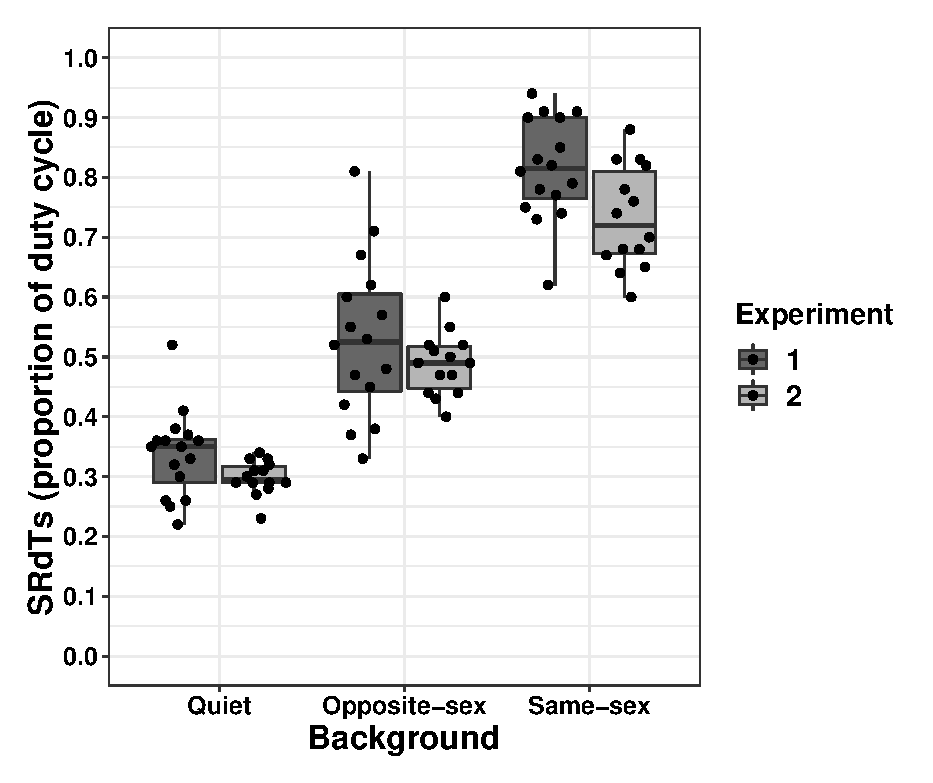
\includegraphics[width=\textwidth]{figures/Chapt1/Boxplot_SK_vs_HW.eps}
\caption{\label{fig:Cmpr_Exp1_2}{Boxplots of the SRdTs obtained in experiment I (dark gray) and experiment II (light gray) for the reference condition Quiet and ENG speech distractor with the same- and opposite-sex talker(s). Individual scores are represented by the black circles.}}
\end{figure}

\hypertarget{score-reproducibility-a-comparison-between-experiment-i-and-ii}{%
\paragraph{Score reproducibility --- a comparison between experiment I and II}\label{score-reproducibility-a-comparison-between-experiment-i-and-ii}}

Next, the reproducibility of the test scores was examined by comparison of the SRdTs obtained in experiment I (dark gray) and II (light gray) for Quiet and ENG speech distractor for same- and opposite-sex distractor talker(s) (see Fig.~\ref{fig:Cmpr_Exp1_2}). No listener participated in both experiments. Overall, the averaged SRdT scores in the two experiments were fairly similar across the different condition, with mean SRdTs of roughly 0.32, 0.51 and 0.78, respectively. Nonetheless, there is a small but noticeable tendency for increased SRdTs (i.e., poorer performance) in the first experiment and for a larger variance when compared with the results in the second experiment.\\

The assumption of normal distribution was fulfilled (Shapiro-Wilk test), however, the assumption of homogeneity of the variance (Levene's test) for the interaction between the two experiments and test conditions Quiet, ENG\(_{same-sex}\) and ENG\(_{ opposite-sex}\)) was not met (\(F(5,84)~=~4.86\), \(p < 0.0001\)). Thus, a nonparametric approach using \textit{nparLD()} function \autocite[nparLD package;][]{nparLDPackageR} was applied to examine the differences in SRdTs between experiments. The function offers a robust rank-based ANOVA-type statistic test (ATS) for analysis of skewed data or for data with outliers or from a small sample size \autocite[see][for a good introduction on robust nonparametric techniques]{Feys2016}. The analysis was based on a f1-ld-f1 design ATS test, which refers to an experimental design with a single between-subjects factor (Experiment: I \& II) and a single within-subject factor (Condition: Quiet, ENG\(_{opposite-sex}\), \& ENG\(_{same-sex}\)). There was no significant interaction between Experiment x Condition (Statistic = 0.412, df = 1.74, \(p = 0.634\)), indicating that performance in the two experiments did not differ between conditions. Whereas there was a highly significant main effect of Condition (Statistic = 271.580, df=1.74, \(p < 0.001\)) and a significant main effect of Experiment (Statistic = 8.260, df = 1.00, \(p < 0.01\)). Nevertheless, the effect-size for Experiment was small with a Cohen's d of 0.264 (95\%-CI: -0.158 - 0.686), whereas the effect-size of condition was large with d ranging between -2.280 to -5.850 \autocite[\textit{effsize::cohen.d()};][]{effsizeRPackage}.\\

\hypertarget{effects-of-the-distractors-language-familiarity-and-talker-sex-on-im}{%
\paragraph{Effects of the distractor's language familiarity and talker-sex on IM}\label{effects-of-the-distractors-language-familiarity-and-talker-sex-on-im}}

A comparison between the listeners' SRdTs measured with the familiar speech distractor (ENG) and the unfamiliar speech distractor (MDR), for same- and opposite-sex distractor talkers, is shown in Fig.~\ref{fig:ENG_vs_MDR}. As before, the diagonal line represents identical performance for the two distractors. The scores were on average very similar in the two distractor-talker configurations, with a DC of roughly 0.5 for opposite-sex and 0.7 for same-sex distractor talkers.\\

The effect of familiarity of the speech distractor was tested using an 2x2x2 factorial design LMEM with repeated measures, with speech distractors as fixed factor (DistrType: ENG \& MDR), distractor talker-sex (DistrTlkrSex: same- and opposite-sex), and the run's order (Order: 1 \& 2) as fixed factors, and subjects as random intercepts (reference levels: ENG\(_{opposite-sex}\), Order=1). The model coefficients and p-values are given in Tab.~\ref{tab:Exp2_LMEM}. A backward model selection, starting from a fully saturated model with three-way interaction for the fixed factors (DistrTlkrSex x DistrType x Order), revealed no significant interaction. The final model did not include interaction terms. Model comparison revealed a highly significant main effect of distractor talker sex (\(p<0.001\)) and a significant effect for familiarity with the language of the speech distractor (\(p=0.029\)), although, the estimated mean difference (0.03) is very small. Similarly, there was a significant main effect of Order (\(p=0.014\)), whilst the overall DC improvement in the second run was again very small (-0.03). The lack of interaction between Order and the other predictors implies that the main effect of Order was the same across the predictors with an overall improvement in the second run. The effect size, Cohen's d, for Order (d = 0.205) was small. The effect size for language was considered ``negligible'' (d = -0.181) and is much smaller than that for the talker-sex (d = -2.494, ``large'').\\

\begin{figure}[ht]
\center
\includegraphics[width=\textwidth]{figures/Chapt1/Exp2_ENG_vs_MDR.PNG}
%\includegraphics[scale=.15]{Exp2_ENG_vs_MDR.PNG}
\caption{\label{fig:ENG_vs_MDR}{SRdTs obtained in experiment II for connected-speech distractors spoken in a familiar language (English, ENG), and an unfamiliar language (Mandarin, MDR) for both same-sex and opposite-sex target/distractor talker configurations. Individual scores are represented by the black circles. The diagonal line represents identical performance for the two speech distractors in the respective distractor talker-sex configuration.}}
\end{figure}

\begin{table}[ht]
\caption{\label{tab:Exp2_LMEM}{2x2x2 mixed-effects model for SRdTs measured in experiment II across all subjects (N~observations $=$ 112; N~Subjects $=$ 13). Significant p-values are marked as bold.}}
\renewcommand{\arraystretch}{2}
\begin{tabular}{lccc}
\hline \hline
\multicolumn{4}{l}{SRdT $\sim$ DistrTlkrSex + DistrType + Order + (1 $\mid$ Subjects)} \\ \hline
Main effects          & Df                        & $\chi^2$ & $p$             \\ \hline
DistrTlkrSex          & 1                         & 151.26   & \textbf{$<$0.001} \\
DistrType             & 1                         & 4.76     & \textbf{0.029}  \\ \hline
Order                   & 1                         & 6.06    & \textbf{0.014}  \\ \hline
Fixed effects         & Estimated mean difference & SE       & 95 \% CI        \\ \hline
intercept             & 0.48                      & 0.02     & 0.44 – 0.52     \\
DistrTlkrSex (same-sex)  & 0.24                      & 0.01     & 0.21 – 0.26     \\
DistrType  (ENG)  & 0.03                     & 0.01     & 0.00 – 0.05   \\
Order  (2)  & -0.03                     & 0.01     & -0.06 – -0.01   \\ \hline \hline
%Random effects        & \multicolumn{3}{c}{Variance}                           \\ \hline
%Subjects (intercept)  & \multicolumn{3}{c}{0.004}                              \\
%Residual              & \multicolumn{3}{c}{0.002}                              \\ \hline \hline   
\\
\end{tabular}
\end{table}

\hypertarget{discussion-1}{%
\subsubsection{Discussion}\label{discussion-1}}

\hypertarget{within-session-test-retest-reliability-1}{%
\paragraph{Within-session test-retest reliability}\label{within-session-test-retest-reliability-1}}

Reliability of the outcome measure is an important requirement for both research and clinical use. Reliability reflects the degree to which a test measure is reproducible when measured by the same listener at different points in time. Low reliability negatively affects the test sensitivity, thus making it difficult to detect difference in scores across different test conditions and/or to distinguish whether the listener's score falls within the normal range \autocite{Cameron2007}.
Test-retest reliability analysis of the listeners SRdTs showed no significant difference between the first and the second run across the different test conditions with estimated mean difference ranging between 0.014 to 0.047. Thus, the switching task appears to provide reliable and reproducible results which is an important requirement for a clinical tool.\\

\hypertarget{score-reproducibility-a-comparison-between-experiment-i-and-ii-1}{%
\paragraph{Score reproducibility --- a comparison between experiment I and II}\label{score-reproducibility-a-comparison-between-experiment-i-and-ii-1}}

Overall, there was a fairly good agreement in SRdTs obtained in experiments I and II across the different test conditions, whereby both experiments showed the same trend of decline in performance when a speech distractor was introduced, with a further decline in performance when the distractor talker was the same sex as of the target talker. Nonetheless, Fig.~\ref{fig:Cmpr_Exp1_2} reveal a small but noticeable positive shift in SRdTs (i.e., poorer performance) as well as a larger variance in the first experiment than in the second experiment. Furthermore, a statistical analysis revealed a significant difference in performance averaged across conditions (p \textless{} 0.01), albeit the effect-size (Cohen's d = 0.264) is considered small.\\

There are several factors that may have contributed to the observed differences in scores. The smaller variability in the SRdTs in experiment II may have been partially as a result of averaging the listeners scores across the two runs, reducing their variability. In experiment I on the other hand, the listeners were presented only once with each test condition. Another, less likely contributing element stems from the different ways the listeners' response was recorded. Typically, in listening tasks that use (non-matrix) everyday sentences, the examiner records the listeners' verbal response. This method was used in experiment II. The self-scoring method we used in the first experiment was deemed lengthy and may have increased the testing error by imposing fatigue and decline in motivation which may explain the overall small trend of poorer SRdTs in experiment I.\\

Nonetheless, probably the most influential factor responsible for the difference in scores may be due to differences in the distractor stimuli. In the first experiment, the speech distractor consisted of a random segment taken from a long passage recorded by a single talker. To maximise the similarity between the target and the distractor, the male talker was chosen to have similar voice characteristics as for the target male voice. In experiment II however, each distractor originated from ten different talkers with a varying voice characteristics, from which a short segment was selected at random every trial. The good agreement in performance between the two experiments in the opposite-sex condition (see Fig.~\ref{fig:Cmpr_Exp1_2}) suggests that when reliable differences in F0 were available, variations in voice characteristics had only a negligible effect on the listener's performance. The IM effect in the opposite-sex distractor talker(s) is likely to be dominated by top-down attentional processing of object-selection, related to target-distractor uncertainty, and may be supported by cues such as phonological cues, semantic content and spatial separation. Such masking interference can take place even when the target and the distractor signals are well formed. The magnitude of the distractor interference also depends on similarity between the two streams in terms of their voice characteristics. Listeners are able to use F0 differences as little as 6\% to considerably improve identification of two simultaneous vowels \autocite{Brokx1982}. F0 cues are known to facilitate speech perception in noise \autocites[e.g.,][]{Binns2007,Miller2010}, helping the listener to easily latch onto the target signal after being ``lost'' by the distractor or by occurrence of an unvoiced speech sound. As for same-sex condition, IM is most likely to be attributed to bottom-up processing, driven by target-distractor similarities (e.g., pitch and prosody) that hinder object formation. One possible explanation for the improved intelligibility in the second experiment may be assigned to the larger set of talkers, resulting in larger variation in talker voice characteristics than in the first experiment which consisted of only a single talker. It is possible that in the second experiment some talkers were more similar to the target talker than others, and that talkers that had less in common with the target talker significantly improved performance when trials were averaged together.\\

\hypertarget{effects-of-distractors-language-familiarity-and-talker-sex-on-im}{%
\paragraph{Effects of distractor's language familiarity and talker sex on IM}\label{effects-of-distractors-language-familiarity-and-talker-sex-on-im}}

One of the main objectives of the second experiment was to examine the role of the semantic content of a distractor on IM in the switching task. The distractor's semantic content was controlled by having distractors spoken in a language that the listeners are or are not familiar with.\\

To our knowledge, no other study has attempted to investigate the components of IM involved in a speech-on-speech listening as presented here; where the target and the distractor signals are interrupted and periodically switched between the two ears out-of-phase with one another. Perhaps the most striking outcome of the first experiment was that only speech distractors impaired task performance. In the absence of a noticeable masking effect for the non-speech distractors, one possible explanation to this is that the ability to ignore a competing talker and to focus on the target talker is hindered by the distractor's semantic content. We therefore hypothesised that the unfamiliar speech distractor in the second experiment will produce smaller masking interference, resulting in better performance than for the familiar speech distractor. However, in contradiction to our expectation, the listeners did not display a masking release when the target speech was presented with an unfamiliar speech distractor (MDR), with only small difference in performance between the two speech types (ENG vs.~MDR). In addition, the non-significant interaction between the distractor type (familiar/unfamiliar) and distractor talker-sex (same/different), indicates that the effect of distractor's talker sex was the same in both distractor types.\\

The findings in the present study corroborate earlier studies \autocite{Freyman2001,Brungart2002,Carlile2015,Summers2020}, and further support the idea that in some more challenging listening tasks, non-energetic/central masking can also be produced for unfamiliar (i.e., non-intelligible) competing speech. The results further confirm the involvement of other factors than semantic content in masking such as MM and attention. Furthermore, although the use of FxNx speech-like distractor in experiment I did not produce a similar masking effect, it would be interesting to see if we can get a similar masker interference in the task using the garbled speech distractor as used by \textcite{Carlile2015} or an unintelligible three-formant buzz-excited vocoded speech as proposed by \textcite{Summers2020}.\\

\hypertarget{general-discussion-and-conclusion}{%
\subsection{General discussion and conclusion}\label{general-discussion-and-conclusion}}

\hypertarget{dichotic-vs.-monotic-presentation-and-the-influence-of-speech-material}{%
\section{Dichotic vs.~monotic presentation and the influence of speech material}\label{dichotic-vs.-monotic-presentation-and-the-influence-of-speech-material}}

\hypertarget{introduction-2}{%
\subsection{Introduction}\label{introduction-2}}

\hypertarget{methods-2}{%
\subsection{Methods}\label{methods-2}}

\hypertarget{results-2}{%
\subsection{Results}\label{results-2}}

To create numbered equations, put them in an `equation' environment and give them a label with the syntax \texttt{(\textbackslash{}\#eq:label)}, like this:

\begin{Shaded}
\begin{Highlighting}[]
\KeywordTok{\textbackslash{}begin}\NormalTok{\{}\ExtensionTok{equation}\NormalTok{\}}\SpecialStringTok{ }
\SpecialStringTok{  f}\SpecialCharTok{\textbackslash{}left}\SpecialStringTok{(k}\SpecialCharTok{\textbackslash{}right}\SpecialStringTok{) = }\SpecialCharTok{\textbackslash{}binom}\SpecialStringTok{\{n\}\{k\} p\^{}k}\SpecialCharTok{\textbackslash{}left}\SpecialStringTok{(1{-}p}\SpecialCharTok{\textbackslash{}right}\SpecialStringTok{)\^{}\{n{-}k\}}
\SpecialStringTok{  (}\SpecialCharTok{\textbackslash{}\#}\SpecialStringTok{eq:binom)}
\KeywordTok{\textbackslash{}end}\NormalTok{\{}\ExtensionTok{equation}\NormalTok{\} }
\end{Highlighting}
\end{Shaded}

Becomes:
\begin{equation}
f\left(k\right)=\binom{n}{k}p^k\left(1-p\right)^{n-k}
\label{eq:binom}
\end{equation}

For more (e.g.~how to theorems), see e.g.~the documentation on \href{https://bookdown.org/yihui/bookdown/markdown-extensions-by-bookdown.html\#equations}{bookdown.org}

\hypertarget{discussion-2}{%
\subsection{Discussion}\label{discussion-2}}

\begin{itemize}
\item
  \emph{R Markdown: The Definitive Guide} - \url{https://bookdown.org/yihui/rmarkdown/}
\item
  \emph{R for Data Science} - \url{https://r4ds.had.co.nz}
\end{itemize}

\hypertarget{conclusion}{%
\subsection{Conclusion}\label{conclusion}}

\hypertarget{Chpt2}{%
\chapter{Spatial listening: development and normalisation of a children's spatialised speech-in-noise test}\label{Chpt2}}

\minitoc 

The magic of R Markdown is that we can add code within our document to make it dynamic.

We do this either as \emph{code chunks} (generally used for loading libraries and data, performing calculations, and adding images, plots, and tables), or \emph{inline code} (generally used for dynamically reporting results within our text).

\hypertarget{introduction-3}{%
\section{Introduction}\label{introduction-3}}

\hypertarget{methods-3}{%
\section{Methods}\label{methods-3}}

\hypertarget{discussion-3}{%
\section{Discussion}\label{discussion-3}}

\hypertarget{conclusion-1}{%
\section{Conclusion}\label{conclusion-1}}

The syntax of a code chunk is shown in Figure \ref{fig:chunk-parts}.

\begin{figure}
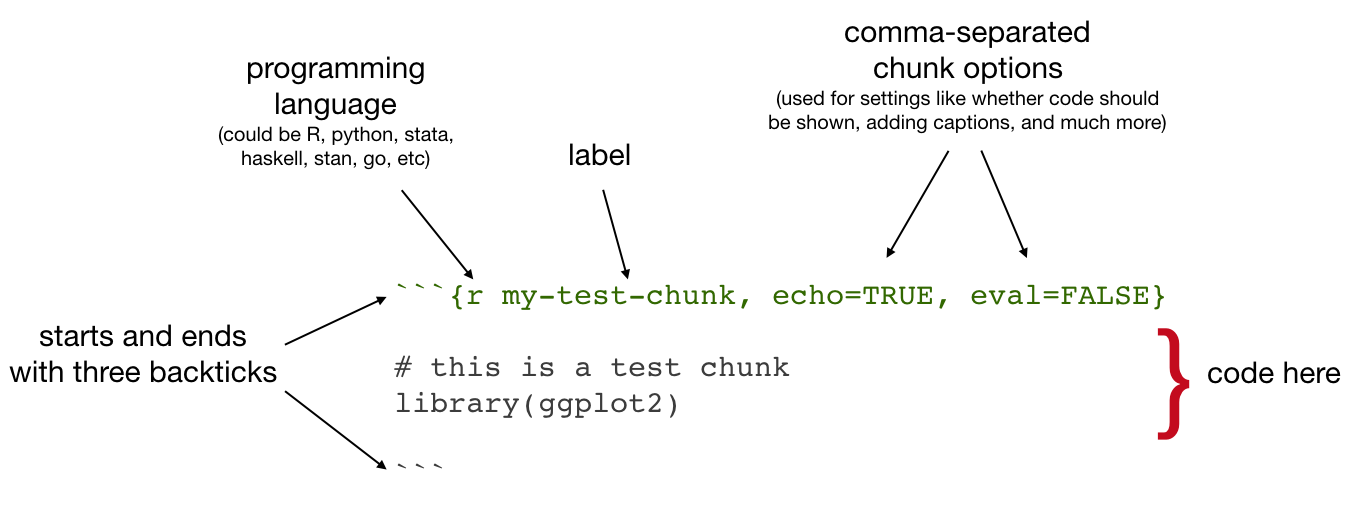
\includegraphics[width=1\linewidth]{figures/chunk-parts} \caption{Code chunk syntax}\label{fig:chunk-parts}
\end{figure}

Common chunk options include (see e.g.~\href{https://bookdown.org/yihui/rmarkdown/r-code.html}{bookdown.org}):

\begin{itemize}
\tightlist
\item
  \texttt{echo}: whether or not to display code in knitted output
\item
  \texttt{eval}: whether or to to run the code in the chunk when knitting
\item
  \texttt{include}: wheter to include anything from the from a code chunk in the output document
\item
  \texttt{fig.cap}: figure caption
\item
  \texttt{fig.scap}: short figure caption, which will be used in the `List of Figures' in the PDF front matter
\end{itemize}

\textbf{IMPORTANT}: Do \emph{not} use underscoores in your chunk labels - if you do, you are likely to get an error in PDF output saying something like ``! Package caption Error: \textbackslash caption outside float''.

\hypertarget{APD-study}{%
\chapter{APD study}\label{APD-study}}

\chaptermark{APD study}

\minitoc 

\hypertarget{introduction-4}{%
\section{Introduction}\label{introduction-4}}

\begin{itemize}
\item
  APD definition: ``unexplained idiopathic (spontanous) listening difficulty (LiD) is often termed auditory processing disorder (APD) in children who have symptoms of difficulty hearing and understanding speech, and abnormal results on more complex auditory tests, despite having normal pure-tone hearing sensitivity (Jerger \& Musiek 2000; Musiek et al., 2017)'' {[}Hunter et al., 2020{]}
\item
  Prevalance of LiD \textasciitilde{} 10\% (Sharma et al., 2009). Prevalence of LiD complaints with measured NH, complying with APD definition is estimated at \textasciitilde0.5 to 1\% of the general population (Hind et al., 2011; Halliday et al., 2017)
\item
  Association with other developmental disorders and lack of understanding of the underlying auditory deficits of APD.
\item
  ``Hearing involves both''bottom-up" (ear to brain) and ``top-down'' (cortical to subcortical) pathways through simultaneous and sequatial processing (Moore \& Hunter, 2013)" {[}Hunter et al., 2020{]}
\item
  Two general mechanistic hypotheses of APD:

  \begin{enumerate}
  \def\labelenumi{(\arabic{enumi})}
  \tightlist
  \item
    \textbf{Sensory processing difficulties (bottom-up)}: involving the central auditory nervous system, are based on animal and human lesion studies (Snow et al., 1997). Supporters of this hypothesis suggested this can be assessed using low-redundancy (simple) speech tests (e.g., using added noise, filtering, rapid speech,..) to ``stress'' the highly redundant central auditory pathways to reveal deficits (Keith 1995, 2000; Cameron et al., 2014).
  \item
    \textbf{Higher-level cognition or attention (top-down)}: especially in children with language disorders (Rees, 1973; Moore et al., 2010).
  \end{enumerate}
\end{itemize}

Individuals may have a combination of both.

\begin{itemize}
\item
  There is no accepted consensus or gold standard diagnosis of APD (Wilson \& Arnott 2013)
\item
  Possible link between OME (+ grommets) or EHF HL and APD in a sub-group of children.
\item
  OME related HL has been shown to persist after recovery at frequencies above 4 kHz (Hunter et al., 2020; REFs..)
\item
  OME or EHF HL can potentially be a basis for poorer speech perception, especially in noise. Findings are not consistent. Studies that tested both TD and APD with OME or EHF HL found that they are predictors of measurable peripheral damage in both groups.

  \begin{itemize}
  \tightlist
  \item
    Besser et al.~(2015) and Levy et al.~(2015) found that better thresholds between 6 to 12.5 kHz were associated with better reception of speech in noise (adult studies).
  \item
    Motlagh Zadeh et al.~(2019): impairment in higher frequency regions could negatively impact speech perception.
  \end{itemize}

  Conductive loss results in impaired spatial processing (Cameron et al., 2014) and binaural interaction (Hall et al., 1995; Hogan et al., 1996)
\end{itemize}

\newpage

\hypertarget{methods-4}{%
\section{Methods}\label{methods-4}}

\hypertarget{participants-2}{%
\subsection{Participants}\label{participants-2}}

Forty-four primary school children who are native British English speakers with normal hearing acuity participated in the study. Amongst them twenty-one belonged to the APD clinical group (5 females) with an average age of 11.04 \(\pm\)~1.42 years (range: 7.8 - 12.9 years). The remaining twenty-three (12 females) comprised of typically developing control children (TD) with no reported concerns or diagnosis of an auditory, language or other cognitive developmental disorder. The TD group average age was 9.47 ±~1.58 years and ranged between 7 to 12.1 years. Since not all the measurement equipment was easily portable and in order to maintain the same environment during the assessment across the complete sample, the children and their caregivers were required to travel to central London for the testing. In order to maximise the number of children taking part in the study, 8 out of the 23 TD children (35\%) had APD siblings which took part in a parallel study on the same day of testing. All the children who participated in the study were required to have normal hearing acuity, defined as thresholds \(\leq\) 25~dB~HL at the octave frequency bands between 0.25 to 8~kHz and their eardrum had to be visible, healthy and intact in both ears following otoscopic inspection. One APD participant was excluded from the analysis due to raised thresholds predominantly in the right ear, ranging between 30 to 45~dB~HL (PTA\(_{Right}\) = 36.25~dB~HL; PTA\(_{Left}\) = 13.75~dB~HL), thus resulting in a final APD group size of twenty. Otoscopic inspection of the child's ear canal revealed a large accumulation of cerumen in both ears with an occluded right ear. Two additional children (x1 APD, x1 TD) had slightly raised thresholds at 8~kHz in one ear of 35 and 30~dB~HL, respectively. However, since thresholds at all other frequency bands were well within the \(\leq\) 25~dB~HL criteria they were not excluded.\\

APD children were recruited in two ways. Children diagnosed with APD at Great Ormond Street Hospital (GOSH) or at the London Hearing and Balance Centre (LHBC), London, UK, were identified based on their clinical records and were contacted by a clinical team member. The caregivers were provided with information about the study and means of contact to express interest in participation. Others, including the TD group were recruited by advertisements on social networks (e.g., APD Support UK Facebook group), science events, local information boards and UCL staff newsletter email, where parents were requested to fill-out an online interest form with short screening questions to ensure that the child met the participation requirements. Most of the children in the APD group (85\%, 17/20) were reported to undergo an APD assessment at GOSH, about a third were directly recruited from the clinic. The remaining three were reported to be assessed at LHBC, at the University of Southampton Auditory Implant Service and Chime Audiology Royal Devon \& Exeter Hospital (screening only).\\

Our initial aim was to take a conservative stance on inclusion criteria by including only those who met a clinical APD criteria (2~SD below the norms on two or more tests during the assessment). Moreover, being aware of the high prevalence of APD children with additional co-occurring developmental disorders, we strived to recruit children who display a ``pure'' form of APD without reported diagnosis or concerns for additional developmental disorder/s. However, very few APD children met these strict criteria, only 75\% (15/20) met the clinical criteria of APD, out of which 60\% (9/15) where diagnosed with spatial processing disorder (SPD) due to abnormal SRM in the LiSN-S task (see Table~\ref{tab:Background-Tab} for descriptives of the APD group). Of the remaining children in the APD group, four did not meet the diagnosis criteria for various reasons (e.g., young age, lack of psychological educational evaluation report and the need to exclude other deficits), however their assessment report acknowledged some ``auditory processing difficulties'', whereas the fifth child awaited an APD assessment following an APD screening. Due to the small sample-size these children were included in the APD group for the analysis, nevertheless, they were subdivided as children with Listening Difficulties (LiD) and differences in performance LiD and APD children were later examined. Furthermore, half of the APD group (10/20) were reported for being diagnosed with one or more secondary developmental disorder/s (x6 Dyslexia, x3 HF-ASD, x3 DLD, x1 ADHD, x1 ADD, x1 Dyspraxia, x1 visual stress, x1 sensory integration disorder, and x1 poor short-term WM). Nonetheless, several caregivers reported that their motivation for seeking additional diagnosis was to get more help from the school, rather than a real concern, after feeling that their support for their child's APD was lacking.\\

\begin{table}

\caption{\label{tab:Background-Tab}APD group demographics and APD-related history background.}
\centering
\begin{tabular}[t]{>{\raggedright\arraybackslash}p{10em}>{\raggedright\arraybackslash}p{20em}}
\toprule
  &  \\
\midrule
\textbf{School type} & 85\% (17/20) Mainstream, (1 child in a special ASD unit, 2 in a private school), 15\% (3/20) non-mainstream school\\
\textbf{Assessment location} & 85\% (17/20) GOSH, 15\% (3/20) other\\
\textbf{APD Diagnosis} & 75\% (15/20) APD, 25\% (5/20) LiD\\
\textbf{SPD subtype} & 60\% (9/15) SPD\\
\textbf{Additional disorder (diagnosed)} & 50\% (10/20) secondery developmental disorder/s\\
\textbf{Additional disorder (undergoing assessment)} & 25\% (5/20)\\
\textbf{OME history} & 60\% (12/20)\\
\textbf{PET history} & 25\% (5/20)\\
\textbf{FM-device usage} & 55\% (11/20)\\
\textbf{Auditory training} & 35\% (7/20)\\
\bottomrule
\multicolumn{2}{l}{\textsuperscript{} OME: Otitis media with effusion}\\
\multicolumn{2}{l}{\textsuperscript{} PET: Pressure equalisation tube}\\
\end{tabular}
\end{table}

Caregivers from both groups completed a comprehensive background questionnaire, similar to the one that is typically given prior to an APD assessment, concerning the caregiver/s educational level, child and family history of hearing, listening problems and developmental disorders, child history of otitis media with effusion (OME), pressure-equalisation tubes (PET / grommets), pregnancy-related questions (e.g., complications, prematurity, etc.), APD-related (e.g., date of diagnosis, location, use of FM device and auditory training), any diagnosis or concerns regarding the child's speech, language, educational and/or cognitive skills, speech and language therapy, medication taken, musical training and the type of school the child attends.\\

Children in the APD group were on average 1.5 years older than children in the TD group. Difference in age between the two groups was tested using t-test with Welch degrees of freedom correction for uneven sample-size \autocite[independent-samples with bootstrapping n=9999; MKinfer package;][]{MKinferPackageR}, showing a significant difference in age between the groups {[}t(40.95) = 3.43, p = 0.001{]}. Nonetheless, since age is often reported as a strong indicator for performance in other similar behavioural studies, analysis of the results obtained in the current study was conducted for age-independent scaled scores and should not affect the comparison between the two groups. The project was approved by the UCL Research Ethics Committee (Project ID Number 0544/006) and the NHS Health Research Authority (REC reference: 18/LO/0250). The testing commenced once an informed consent was given by both the caregiver and the child.

\hypertarget{measurements}{%
\subsection{Measurements}\label{measurements}}

The test battery used in the present study is described in the following section and summarised in Table~\ref{tab:Methods-Tab}.

\begin{table}

\caption{\label{tab:Methods-Tab}Summary of the study test battery.}
\centering
\resizebox{\linewidth}{!}{
\fontsize{9}{11}\selectfont
\begin{tabular}[t]{>{\raggedright\arraybackslash}p{12em}>{\raggedright\arraybackslash}p{24em}>{\raggedright\arraybackslash}p{10em}}
\toprule
\textbf{Task} & \textbf{Information} & \textbf{Measure}\\
\midrule
\textbf{Standard \& extended high-frequency (EHF) audiometry} & Pure-tones detection thresholds measured at the octave frequency bands between 0.25 and 8 kHz (standard), and 8 to 20 kHz (EHF). & Detection threshold in dB HL\\
\textbf{Switching task (ST)} & Adaptive speech-on-speech listening task that involves perception of interrupted and periodically segmented speech that is switched between the two ears out-of-phase with an interrupted distractor. ST assesses the ability to switch attention and integration of binaural information. & Proportion of speech required to understand 50\% of the keywords, Speech Reception duty cycle Threshold (SRdT)\\
\textbf{Listening in Spatialised Noise Sentences UK (LiSNS-UK)} & Locally developed version of the LiSN-S (Cameron \& Dillon, 2007), an adaptive speech-on-speech listening task that assesses the ability to use spatial release from masking (SRM), measured as the difference in perception between collocated and separated speech distractors. & Signal-to-noise-ratio (SNR) yielding 50\% speech intelligibility, Speech Reception Threshold (SRT)\\
\textbf{Speech-shaped-noise (SSN)} & Conventional adaptive speech in noise task that asseses speech perception of ASL sentences (MacLeod \& Summerfield, 1990) in a speech-shaped-noise with a spectrum matched to the ASL material. & SRT\\
\textbf{The Environmental Auditory Scene Analysis task, ENVASA} (Leech et al., 2009) & Non-linguistic self-administered task involves detection of everyday environmental sounds presented in naturalistic auditory scenes and can be used to asses IM effects as well as sustained selective auditory attention skills. & \%-correct\\
\textbf{Recalling sentences, CELF-RS} (Wiig et al., 2017) & A subtest from the Clinical Evaluation of Language Fundamentals UK 5$^{th}$  edition (CELF-5-UK), assess expressive language skills, measured by the ability to repeat in verbatim sentences with varying length and complexity. Standardised for children aged 5 to 16 years. & Age-corrected scaled scores\\
\textbf{The Evaluation of Children's Listening and Processing Skills, ECLiPS} (Barry \& Moore, 2014) & Standardised questionnaire comprises of 38  statements grouped into five categories designed to identify listening and communication difficulties in children aged 6 to 11 years. Respondents agreement is expressed using a five-point Likert scale ("\textit{strongly agree}" - "\textit{strongly disagree}"). & Age-corrected scaled scores\\
\textbf{The Children's Communication Checklist 2$^{nd}$ edition, CCC-2} (Bishop, 2003) & Standardised questionnaire comprisng of 70 items designed to screen language and/or communication problems in children aged 4 to 16 years. Item comprises of a behaviour statement (e.g., "\textit{Mixes up words of similar meaning}") with respondents asked to judge how often the behaviours occur using a four-point Likert scale (0-3). & Age-corrected scaled scores\\
\bottomrule
\end{tabular}}
\end{table}

\hypertarget{auditory-evaluation}{%
\subsubsection{Auditory evaluation}\label{auditory-evaluation}}

\hypertarget{standard-extended-high-frequency-ehf-audiometry}{%
\paragraph*{Standard \& extended high-frequency (EHF) audiometry}\label{standard-extended-high-frequency-ehf-audiometry}}
\addcontentsline{toc}{paragraph}{Standard \& extended high-frequency (EHF) audiometry}

\hfill\break
Otoscopic inspection was performed prior to the audiometric test to ensure the ear was clear from cerumen and to avoid harming the eardrum when inserting the ear probe. Both standard and extended high-frequency (EHF) audiometry thresholds were measured using the Hughson-Westlake manual procedure, starting from 1~kHz. Standard air conduction pure-tone audiometry was carried out at six octave frequency bands ranging between 0.25 to 8~kHz using ???? audiometer and ??? headphones.\\

Extended high-frequency pure-tone detection thresholds were measured at four octave frequency bands 8, 11, 16, \& 20~kHz using locally written MATLAB based software which generated the stimulus and collected the data. Target tones were pulsed (3 repetitions) with a duration time of 700~ms and 50~ms rise/fall time. EHF measurements took place in a designated sound attenuated chamber with the child sitting in the centre of the chamber while the examiner was situated outside. Communication during the testing was carried out via a video-audio intercom system. The child was instructed to raise his/hers hand each time s/he heard a tone. The MATLAB script was executed using a Windows PC which which was connected via USB to an RME ???? sound card (Audio AG, Haimhausen Germany) and an ER10X Extended-Bandwidth Acoustic Probe System (Etym\(\bar{o}\)tic Research, Elk Grove Village, IL). Stimulus was presented via an otoacoustic emission probe with silicon tips in variable sizes (between 10 to 13~mm), depending on the size of the child's ear.\\

Standing waves in the ear canal produces spatially non-uniform sound pressure at frequencies above 2-3~kHz, introducing calibration errors when estimating the sound pressure level arriving at the eardrum \autocite{Siegel1994,Richmond2011,Lee2012}. Together with other factors such as individual variations in the ear canal length and differences in depth in which the ear probe is inserted into the ear canal, these factors can introduce up to 20~dB calibration error \autocite{Siegel1994}. To account for that, a sound pressure level calibration procedure was used (chirp noise) using a similar technique as described by \textcite{Lee2012}. For each frequency, the first half-wave resonance of the ear canal was measured, estimating the distance between the ear probe and the eardrum. The target stimulus was then scaled to the desired output level that corresponds to 0~dB~HL using the in-situ calibration forward-pressure level data (FPL) and EHF-specific weighting thresholds (in dB SPL) measured across 84 NH listeners aged 10 to 21 years \autocite[see Table 1 in][]{Lee2012}.

\hypertarget{switching-task-st}{%
\paragraph{Switching task (ST)}\label{switching-task-st}}

\hfill\break
Estimating the effect of IM while minimising peripheral EM on speech perception was measured using the switching task (ST) which is believed to assess the listeners ability to switch attention and integration of binaural information. The exact same test procedure and equipment was used as described in Chapter~\ref{Chpt1}. Listeners were presented with both test versions using the ASL and the CCRM speech material. As for the stimuli, the ASL target sentences, spoken by a single male talker, were taken from the final sentences selected following the normalisation study. In addition, a level correction was applied to each sentence using the sentence-specific weighing factors estimated in the normalisation study (see Chapter~\ref{Chpt2}). The first five test lists out of the eight phonetically-balanced normalised test lists (\(\grave{a}\) 25 sentences each) were used, whereby their order was quasi-randomised to account for order, masker combinations, and fatigue effect. The target CCRM sentences were the same as described in Chapter~\ref{Chpt1}, spoken by three different male talkers, were selected at random every trial and always began with the priming animal `dog'. The target speech material was presented either without a distractor (Quiet) with and without switching (NoAlt / Alt) or with a distractor. A selection of four distractors were used (see Chapter~\ref{Chpt1} for detailed description): English (ENG\_F) and Mandarin (MDR\_F) unrelated connected-speech, each spoken by ten different female talkers, and a non-speech amplitude-modulated speech-spectrum-noise (AMSSN) with the envelope of a single talker out of 40 talkers (20 females). The fourth distractor was presented only with the CCRM speech material and comprised of CCRM target-like sentences (CCRM\_F) with a different priming animal, colour and digit, spoken by ten different female talkers. Each participant was presented with a total of 11 runs, one for each test condition, with 5 conditions for the ASL (Quiet-NoAlt,Quiet-Alt, MDR\_F-Alt, ENG\_F-Alt), and 6 for the CCRM (with the additional CCRM\_F-Alt condition). Testing started following a practice phase, where four trials of each of the eleven test conditions were presented. Practice runs started at an easy-to-moderate DC rate of 0.8 in order to expose the listeners to the adaptive procedure. In addition, every test run started with two practice sentences (initial DC = 0.97) to orient the listeners to the test condition that is about to be presented.\\

\hypertarget{listening-in-spatialised-noise-sentences-uk-lisns-uk}{%
\paragraph{Listening in Spatialised Noise Sentences UK (LiSNS-UK)}\label{listening-in-spatialised-noise-sentences-uk-lisns-uk}}

\hfill\break
The locally developed Listening in Spatialised Noise Sentences UK (LiSNS-UK) assesses the ability to use binaural cues in speech-on-speech listening conditions. The test development, speech material normalisation, and norms standardisation followed \textcite{Cameron2007} development steps and are described in detail in Chapter~\ref{Chpt2}. The test uses virtualisation techniques to create spatial distribution of sound sources in space for headphones presentation where target sentences \autocite[ASL;][]{MacLeod1990} are presented in two simultaneous speech distractors (unrelated children's stories spoken by the target talker). The LiSNS-UK comprises of two main listening conditions, differing in their availability of spatial cues. The target sentences are configured to always appear in front of the listener's head, at 0\(^{\circ}\) azimuth on the horizontal plane, with the two streams of speech distractors either collocated in space with the target (S0N0), resulting in relatively poor speech perception, or offset in space, with one distractor to either side of the target at \(\pm\)~90\(^{\circ}\). The spatial separation in the later condition results in an improvement in speech perception of circa 13~dB \autocite{Cameron2011}, typically termed as spatial release from masking (SRM). This SRM advantage is calculated by taking the difference between performance in the collocated and the separated condition.\\

Speech distractors were presented continuously throughout a run at a fixed 65~dB~SPL output level and comprised of a combination of two out of three available passages. A 1-up/1-down adaptive procedure was used, varying the level of the target talker relative to the distractors depending on the listener's response to measure their speech reception threshold (SRT), i.e., the signal-to-noise-ratio (SNR) yielding 50\% speech intelligibility. A 2~ms long reference cue (1~kHz pure-tone) was presented 500~ms before the target sentence onset at 65~dB~SPL. The initial target output level was 75~dB~SPL for the collocated condition and 70~dB~SPL for the separated condition with an initial step-size of 4~dB SNR. The step-size was reduced after every reversal, reaching a minimum step-size of 2~dB~SNR after three practice reversals. The adaptive procedure ended once all 25 test trials were presented and stopped in case a maximal output level of 89~dB~SPL was reached more than three times. Nonetheless, such event did not occur in the present study. Since each listener was only presented once with each condition, it was decided not to introduce any other stopping rules that could have expedited the testing time but may as well introduced an estimation error for the SRTs in some cases. The SRT was calculated by averaging the test reversals SNRs, whereby test reversals were defined as any reversals following three practice reversals.\\

The order of the listening condition, test lists, sentences within a run, and distractors combinations was fixed across all the participants and started with the collocated condition. Each test list consisted of 25 sentences taken from the 8-phonetically-balanced ASL test lists which were constructed following the normalisation study and a sentence-specific level correction was applied (see Chapter~\ref{Chpt2}). Spatialisation was applied by convolving each stimuli with head-related transfer functions (HRTFs) at the corresponding azimuthal direction separately for the left and the right channel. The HRTFs were measured with a Knowles Electronics Manikin for Acoustic Research (KEMAR) with a small pinnae taken from the CIPIC HRTF database\footnote{The database is available online in: \url{https://www.ece.ucdavis.edu/cipic/spatial-sound/hrtf-data/}} \autocite[see][``special'' HRTF data]{Algazi2001}. A post-equalisation step was applied in order to flatten the magnitude of the headphones frequency response. Headphone-to-ear Transfer Functions (HpTFs) measured with KEMAR manikin for HD-25 supraaural headphones were extracted from \textcite{Wierstorf2011} HRTF database. The final mixed stimulus was filtered with the inverse HpTFs separately for the left and the right channel before being combined together as a final step. Every participant was presented with two runs, one for each listening condition (collocated / separated). Testing started following a practice phase of two runs, one for each of the test conditions with five BKB sentences each \autocite{Bench1979}. Listeners were instructed to verbally repeat the target sentences to the experimenter who was situated alongside in a sound treated chamber. The experimenter scored the response by selecting the correctly repeated keywords on the screen. Listeners were encouraged to guess if unsure while no feedback was given at any time. A loose keyword scoring method was used, whereby errors of case or declension were considered as correct responses, e.g., a repetition of the keywords `\(<\)clown\textbf{s}\(>\) \(<\)funny\(>\) \(<\)face\textbf{s}\(>\)' to the stimulus `The \(<\)clown\(>\) had a \(<\)funny\(>\) \(<\)face\(>\)'.

\hypertarget{speech-shaped-noise-ssn}{%
\paragraph{Speech-shaped-noise (SSN)}\label{speech-shaped-noise-ssn}}

\hfill\break
A speech-in-noise test was used as a more conventional listening task that is widely used in the clinic as opposed to the more complex listening conditions measured by the ST or the LiSNS-UK. The normalised ASL sentences were presented in a speech-spectrum-noise (SSN) with spectrum matched to the ASL corpus. The SSN onset was 500~ms before the target sentence began. The exact same adaptive procedure as for the LiSNS-UK was used with the same stopping-rules and SRT calculation. Each listener was presented with a single run of 25 sentences following a practice phase with seven BKB sentences. The same test list and sentences order was used across all the listeners.

\hypertarget{the-environmental-auditory-scene-analysis-task-envasa}{%
\paragraph{The Environmental Auditory Scene Analysis task (ENVASA)}\label{the-environmental-auditory-scene-analysis-task-envasa}}

\hfill\break
In analogy to the classic `cocktail-party' scenario, ENVASA is a non-linguistic paradigm \autocite{Leech2009} that measures detection of everyday environmental sounds presented in naturalistic auditory scenes and can be used to asses IM effects as well as sustained selective auditory attention skills. In the task, short environmental target sounds (e.g., a dog's bark, a door knock, or a bouncing ball) were presented in a dichotic background scene (i.e., the target sound is presented only in one ear), consisting of either a single background scene, presented in both ears, or two background scenes, each presented in a different ear. The number of targets, the onset time and the ear of presentation varied across trials. Four SNRs were employed split into two categories `low' (-6 and -3~dB) and `high' (0 and +3~dB). Target-background contextual agreement was manipulated by embedding the target sound in a \emph{congruent} background scene that is in agreement with the listener's expectations (e.g., a cow's `moo' in a farmyard scene) or in an \emph{incongruent} background scene which violate these expectations (e.g., a cow's `moo' in a traffic scene). A schematic illustration of a single test sequence is shown in Figure \ref{fig:ENVASA}.\\

The experiment was carried out using the original setup as described by \textcite{Leech2009}. Sounds were presented via Sennheiser HD-25 headphones (Wedemark, Germany) and the participants response was recorded using ???? gamepad. The output level was adjusted to a comfortable level before the test started. The participants were situated in front of a laptop and were instructed to hold the gamepad. Prior to the test, the listeners were presented with a short child-friendly demonstration video with audio instructions. Next, a short recap was given verbally by the examiner and an exemplary trial was simulated together with the child to ensure that the child fully understood the task's instructions. The task began with three short practice trials with provided feedback, while no further feedback was given during the test phase.\\

Every trial was made of two parts, starting with a target audio and visual familiarisation phase before the main target detection phase. Target identification was recorded by pressing one of the three buttons on the gamepad which corresponded to the location of the target objects on the screen. A response was counted as correct only if the participants pushed the corresponding button within 2 seconds, 300~ms after the target onset. The outcome measure was calculated as the percentage of target sounds correctly identified within a condition (\%-correct). In total there were 115 target sounds presented over 40 trials, where 46 target sounds were presented in a single background condition and another 46 in a dual-background condition. The 23 remaining target sounds served as foil items which were played at 0~dB~SNR without a corresponding picture on the screen. The order of the foil items was quasi-randomised and was used to estimate the quality of the participants performance.\\



\begin{figure}

{\centering 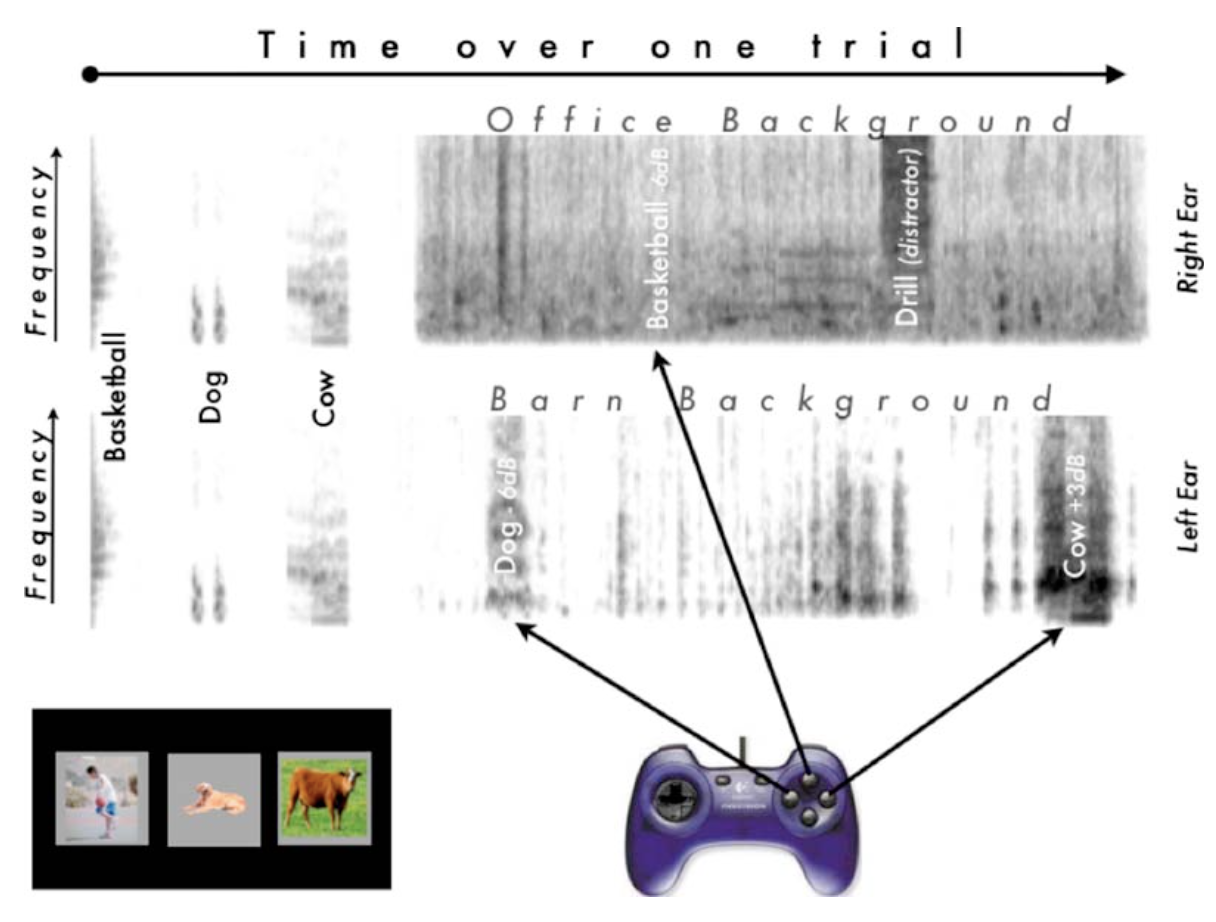
\includegraphics[width=0.65\linewidth]{figures/ENVASAparadigm} 

}

\caption{Schematic of the ENVASA experimental paradigm \autocite[taken from][]{Leech2009}}\label{fig:ENVASA}
\end{figure}

\hypertarget{celf-rs}{%
\paragraph{CELF-RS}\label{celf-rs}}

\hfill\break
The Recalling Sentences (RS) sub-test of the Clinical Evaluation of Language Fundamentals UK fifth edition \autocite[CELF-5-UK;][]{HWiig2017} was administered to assess the listeners expressive language skills, measuring the ability to repeat in verbatim sentences with varying length and complexity. Standardised norms are available for children aged 5 to 16 years. The CELF-RS is simple and quick to administrate and has been shown to be a good psycholinguistic marker for children with Developmental Language Disorder (DLD) and to provide high levels of sensitivity and specificity \autocite{Conti-Ramsden2001}, thus making it a good screening tool. Scoring were marked by hand by the examiner as instructed by the test manual. The sentences were presented using a local MATLAB program via headphones using the same experimental equipment as listed above at a comfortable output level of 70~dB~HL. The sentences were spoken by a female speaker with a standard southern British English accent and were recorded in a sound-treated recording booth at the Speech, Hearing and Phonetics Sciences (SHaPS), UCL laboratory, London. The task began with two practice sentences while the number of test items varied depending on the child's age and performance. No repetitions or feedback was given during the testing and the test was discontinued in case the child failed to score any points for four consecutive items. Age-scaled score were calculated based on the test norms with a mean score of 10 and SD of 3. Scaled scores within \(\pm\)~1~SD from the norms mean (between 8 to 12) are classified as average scores, whereas performance beyond \(\pm\)~1~SD are classified as above / below the average score, with scaled-scores \textless~7 considered as abnormally poor.\\

\hypertarget{questionnaires}{%
\subsubsection{Questionnaires}\label{questionnaires}}

\hypertarget{the-evaluation-of-childrens-listening-and-processing-skills-eclips}{%
\paragraph{The Evaluation of Children's Listening and Processing Skills (ECLiPS)}\label{the-evaluation-of-childrens-listening-and-processing-skills-eclips}}

\hfill\break
The ECLiPS questionnaire \autocite{Barry2014} comprises of 38 items, where the respondents are asked to express their agreement on simple statements about the child's listening and other related skills or behaviours using a five-point Likert scale (from ``strongly agree'' to ``strongly disagree''). The ECLiPS was design to identify listening and communication difficulties in children aged 6 to 11 years. Nonetheless, in their evaluation study, \textcite{Barry2014} found little to no age effect in many of the scale items, suggesting that testing age could be extended below and beyond the population used for the development. Based on factor analysis the items were grouped into five subcategories: 1. Speech \& Auditory Processing (SAP), assessing ability to interpret speech and non-speech input, 2. Environmental \& Auditory Sensitivity (EAS), estimating the ability to cope with environmentally challenging conditions, 3. Language, literacy \& laterality (L/L/L), assessing different abilities that are known to be coupled with language and literacy difficulties, 4. Memory \& Attention (M\&A), covering short-term and serial memory as well as attention, 5. Pragmatic \& Social skills (PSS), assessing pragmatic language or non-normative social behaviours. Aggregated measures were calculated for \emph{Listening} (SAP, M\&A, \& PSS), \emph{Language} (L/L/L \& M\&A), \emph{Social} (PSS \& EAS), and a \emph{Total} aggregate, calculated by taking the mean of scores across all the sub-scales. Individual age- and sex-scaled scores were computed using the test excel scorer. A score below the 10\(^{th}\) percentile (corresponding to a scale score of circa 6) is generally considered clinically significant.\\

\hypertarget{the-childrens-communication-checklist-2nd-edition-ccc-2}{%
\paragraph{\texorpdfstring{The Children's Communication Checklist 2\(^{nd}\) edition (CCC-2)}{The Children's Communication Checklist 2\^{}\{nd\} edition (CCC-2)}}\label{the-childrens-communication-checklist-2nd-edition-ccc-2}}

\hfill\break
Communication abilities were assessed using the Children's Communication Checklist second edition questionnaire \autocite[CCC-2;][]{Bishop2003} which is designed to screen communication problems in children aged 4 to 16 years and comprises of 70 checklist items each comprising of a behaviour statement, like ``\emph{Mixes up words of similar meaning}''. The respondents are asked to judge how often the behaviours occur using a four-point Likert rating scale: 0. \emph{less than once a week (or never)}, 1. \emph{at least once a week, but not every day}, 2. \emph{once or twice a day}, 3. \emph{several times (more than twice) a day (or always)}. The items are grouped into ten sub-scales of behaviours tapping into different skills (A. Speech, B. Syntax, C. Semantics, D. Coherence, E. Inappropriate initiation, F. Stereotyped language, G. Use of context, H. Non-verbal communication, I. Social relations, J. Interests). Taking the sum of scores for the sub-scales A to H are used to derive the General Communication Composite (GCC) which is used to identify clinically abnormal communication competence. A GCC score \textless{} 55 was found to well separate between control and clinical groups, identifying children with scores at the bottom 10\% \autocite{Norbury2005}. Another proposed composite, is the SIDC (Social-Interaction Deviance Composite) which is calculated by taking the difference in sum of subscales E, H, I, and J (tapping into pragmatic language and social skills) from the sum of scales of A to D (describes structural language skills). Abnormal GCC (\textless~55) combined with a negative SIDC score has been shown to be indicative of an autistic spectrum disorder profile \autocite{Bishop2003}. The CCC-2 scaled and composite scores were computed using the test scorer.\\

\hypertarget{procedure-2}{%
\subsection{Procedure}\label{procedure-2}}

Testing took place at the SHaPS laboratory (UCL, London) in a sound-attenuated chamber. Unfortunately, since many of the APD children had to travel from outside London and because of difficulties in recruitment, all the testing had to be made in a single session, lasting in total circa 2.5 to 3 hours (including breaks). To minimise possible fatigue effect, the session was carefully designed to ensure several planned and unplanned brakes. The participants were encouraged to request for a break between test runs whenever they required and were observed for any signs of fatigue by the examiner. The different tasks were gathered into short blocks and different measures were scattered throughout the session to keep the session fun and engaging for the child. At the end of the session, each child received a certificate and an Amazon voucher as a token of appreciation for taking part in the study and travel costs of the family were reimbursed.\\

Participants from both the TD and the APD group completed the same test battery in the below listed order (see Table \ref{tab:Study-Procedure}). Th ECliPS, CCC-2 and the locally compiled background questionnaire were completed by the caregiver during the testing day. The session started with a standard pure-tone audiogram and otoscopy to ensure that detection thresholds fulfil the study criteria and that there are no abnormalities in the ear canal and the eardrum. Next, the switching task was conducted. Since performance in the task was one of the main focuses in the study, and because little is known about any possible learning effect in the task, presentation of the two speech materials (ASL and CCRM) was counterbalanced within each group, where about half of the children started with the ASL and the other half with the CCRM speech material. In between the two ST versions, each child completed the CELF-RS and the SSN task, whereby again, the order of presentation was counterbalanced within each group. Since both CELF-RS and SSN test duration are relatively short, they served as a short informal break between the ST test versions and kept the child engaged. Next, about half-way through the session, with a fixed order, all the participants were presented with the EHF audiometry, and the ENVASA task. The session was concluded with the LiSNS-UK, in-line with typical clinical assessment where the test is often presented last.\\

\begin{table}

\caption{\label{tab:Study-Procedure}Experimental design and measurements order.}
\centering
\resizebox{\linewidth}{!}{
\fontsize{8}{10}\selectfont
\begin{tabular}[t]{lllll}
\toprule
Order & Group A & Group B & Group C & Group D\\
\midrule
1 & Otoscopoy & Otoscopoy & Otoscopoy & Otoscopoy\\
2 & Standard audiometry & Standard audiometry & Standard audiometry & Standard audiometry\\
3 & ST-ASL & ST-ASL & ST-CCRM & ST-CCRM\\
4 & CELF-RS & SSN & CELF-RS & SSN\\
5 & ST-CCRM & ST-CCRM & ST-ASL & ST-ASL\\
6 & SSN & CELF-RS & SSN & CELF-RS\\
7 & EHF audiometry & EHF audiometry & EHF audiometry & EHF audiometry\\
8 & ENVASA & ENVASA & ENVASA & ENVASA\\
9 & LiSNS-UK & LiSNS-UK & LiSNS-UK & LiSNS-UK\\
\bottomrule
\end{tabular}}
\end{table}

\hypertarget{data-analysis}{%
\subsection{Data Analysis}\label{data-analysis}}

All the data extraction, management and analysis in the present study was computed in R environment \autocite[Version 4.0.3;][]{RCore} using RStudio \autocite[Version 1.4.938;][]{RStudio}.\\

\hypertarget{z-scores}{%
\subsubsection{Age scaled scores}\label{z-scores}}

Age-independent scores were estimated using a linear regression model. The model was fitted per condition separately for each measure (ST-ASL, ST-CCRM, LiSNS-UK, SSN, \& ENVASA) and was based on the control group data only with the respective test raw scores (e.g., SRdT, SRT or \%-correct) as an dependent variable and age as a predictor. A two-steps model comparison was performed to test the assumption that performance displays a monotonic linear relationship with age versus a non-monotonic (segmented) linear relationship. Extreme outliers were initially trimmed from the TD group to reduce noise in the data and to improve the models fit. In the first step, both models were computed and the best model was selected based on F-statistic model comparison using analysis of variance using \emph{anova()} function. Standard residuals were next calculated for each TD listener, based on the selected model prediction. Since age was included in the model, the standardised residuals are age-independent and are comparable to z-scores for data with normal distribution, with a mean and SD of approximately 0 and 1. Since the main goal of the study was to find a measure that is able to well separate between the APD group and the typically developed control group, individual differences and group differences were explored using a deviance analysis procedure proposed by \textcite{Ramus2003}. Abnormal scores were defined by a two-tailed deviance cut-off of \(\pm\)~1.96~SD from the TD group mean. Thus, circa 95\% of the normal population residuals are expected to be within the deviance range of \(\pm\)~1.96. Occasional occurrence of abnormal scores in the normal population is not unusual in behavioural measures. Therefore, since the prediction of the residuals is based on the control data, such outliers may skew the TD group true mean or SD and thus may introduce an error in the model prediction. Therefore, in the second step, additional TD outliers (with standardised residuals below/above TD mean \(\pm\)~1.96) were trimmed from the data and the two models were refitted and compared again. Finally, the model with the best fit was selected and was used to calculate the standardised residuals for all the listeners, including the trimmed TD observations and the APD group.

\hypertarget{statistical-analyses}{%
\subsubsection{Statistical analyses}\label{statistical-analyses}}

Residual analysis was performed separately for each measure to determine whether the data fulfils parametric methods assumptions of normal distribution using Shapiro-Wilk test \autocite[\emph{shapiro.test()},][]{RCore} and homogeneity of variance using Levene's test \autocite[\emph{leveneTest()};][]{carPackageR}. Consequently, statistical analyses for factorial design data that met these requirement was performed using linear mixed-effects regression models (LMEMs). LMEM was fitted using the \emph{lmer()} function \autocite[lme4 package;][]{lme4PackageR}. Backward model selection procedure was applied to find the model that gives the best fit using a likelihood ratio test (\(\chi^2\)). Main effects and interaction terms were tested by comparing predictions of the full model to a reduced model where each fixed term was separately removed, starting with the interaction terms. When applicable, post-hoc paired comparison t-test was performed on the fitted model and included adjusted least-squared-mean for the random intercepts (subjects) using the \emph{lsmeans()} function from the emmeans R package \autocite{emmeansPackageR}. In addition, group differences for single parametric measures such as CELF-RS and CCC-2 total score were examined using \emph{boot.t.test()} function \autocite[MKinfer package;][]{MKinferPackageR} which performs independent-samples t-test with bootstrapping (n=9999).\\

Nonparamertic data was analysed using nparLD() function \autocite[nparLD package;][]{nparLDPackageR} which is a robust rank-based method for analysis of skewed data or for data with outliers or from a small sample size \autocite[see][ for a good introduction on robust nonparametric techniques]{Feys2016}. The function enables different types of nonparametric tests for factorial design data with repeated measures with variable between-/within-subjects factors. The results reported in the present study were based on the ANOVA-type statistic test (ATS) output. Inspection of the ENVASA task age-independent z-scores revealed that the assumption of sphericity (Mauchly's test) was violated. Therefore, analysis was performed using \emph{npIntFactRep} package \autocite{npIntFactRepPackageR}, which is another robust aligned rank technique that enables sphericity correction (Greenhouse-Geisser). When applicable, post hoc comparison and group difference were examined using Wilcoxon rank-sum test with permutation (N=999999, independent two samples) which is a t-test equivalent for non-parametric data \autocite[\emph{coin::wilcox\_test()};][]{CoinPackageR}.

\hypertarget{results-3}{%
\section{Results}\label{results-3}}

\hypertarget{standard-audiometry}{%
\subsection{Standard audiometry}\label{standard-audiometry}}

The listeners' detection thresholds for the left and the right ear are plotted in Figure~\ref{fig:PTA}. The shaded grey area represents the TD group thresholds range and the white line represents the group mean at each frequency. The black lines marks the individual thresholds in the APD group and the group mean is marked by the bold black line. The dashed line indicates the maximal thresholds criteria of \(\leq\) 25~dB~HL for participation in the study.\\

\begin{figure}

{\centering \includegraphics[width=0.85\linewidth]{_main_files/figure-latex/PTA-1} 

}

\caption{Standard audiometry: APD participants pure-tone detection thresholds plotted seperately for the left and the right ear (black lines). The shaded grey area represents the TD group thresholds range and the white line represents the TD group mean at each frequency. The dashed line represents the threshold criteria of hearing level $\leq$ 25 dB HL.}\label{fig:PTA}
\end{figure}

Boxplots of listeners pure-tones detection thresholds measured at six octave frequency bands between 0.25 to 8~kHz and their corresponding pure-tone-average (PTA) are shown in Figure~\ref{fig:RegAud-fig}~A-B. Individuals PTAs were calculated by averaging thresholds at the frequency bands 0.5, 1, 2 and 4~kHz separately for the right and left ear (PTA\(_{Right}\), PTA\(_{Left}\)) and by taking the grand mean for thresholds in both ears (denoted as PTA), whereas the listeners' PTA at the better-ear is denoted as BE. Thresholds descriptives by frequency bands and ear split by the two groups is given in Table~\ref{tab:RegAud-Tab1}, as well as Table~\ref{tab:RegAud-LMEMpost} for PTAs and BE with additional statistics.\\

\begin{figure}

{\centering \includegraphics[width=1\linewidth]{_main_files/figure-latex/RegAud-fig-1} 

}

\caption{Standard audiometry: Pure-tone detection thresholds by frequency bands between 0.25 to 8 kHz (A), and averaged thresholds (B). Individual scores are indicated by circles. The boxes show the data interquartile range (25th-75th percentile) and the horizontal line indicate the median (i.e., 50th percentile). Values that fall within 1.5 times the interquartile range are indicated by the wiskers.}\label{fig:RegAud-fig}
\end{figure}

\begin{table}

\caption{\label{tab:RegAud-Tab1}Standard audiometry: Descriptives for pure-tone detection thresholds (dB HL) by frequency bands (kHz) and ear split by the two groups.}
\centering
\resizebox{\linewidth}{!}{
\begin{tabular}[t]{lcccccc|>{}ccccc}
\toprule
\multicolumn{2}{c}{ } & \multicolumn{5}{c}{APD} & \multicolumn{5}{c}{TD} \\
\cmidrule(l{3pt}r{3pt}){3-7} \cmidrule(l{3pt}r{3pt}){8-12}
Frequency & Ear & N & median & sd & min & max & N & median & sd & min & max\\
\midrule
0.25 & R & 20 & 10 & 3.73 & 0 & 15 & 23 & 5 & 3.95 & 0 & 15\\
0.5 & R & 20 & 5 & 4.94 & 0 & 15 & 23 & 10 & 4.49 & -5 & 15\\
1 & R & 20 & 5 & 4.55 & -5 & 15 & 23 & 0 & 4.38 & -5 & 15\\
2 & R & 20 & 5 & 3.97 & 0 & 15 & 23 & 5 & 3.76 & 0 & 10\\
4 & R & 20 & 5 & 5.62 & -5 & 15 & 23 & 5 & 5.27 & -5 & 15\\
8 & R & 20 & 10 & 5.36 & 0 & 20 & 23 & 10 & 8.29 & -5 & 30\\
\midrule
0.25 & L & 20 & 5 & 4.99 & 0 & 20 & 23 & 5 & 5.05 & -5 & 15\\
0.5 & L & 20 & 10 & 4.06 & 5 & 15 & 23 & 5 & 4.25 & -5 & 15\\
1 & L & 20 & 5 & 3.84 & 0 & 15 & 23 & 0 & 3.99 & -5 & 10\\
2 & L & 20 & 5 & 4.13 & 0 & 15 & 23 & 0 & 4.03 & -5 & 10\\
4 & L & 20 & 5 & 5.95 & -5 & 15 & 23 & 5 & 6.07 & -5 & 20\\
8 & L & 20 & 10 & 8.01 & 5 & 35 & 23 & 5 & 8.49 & -5 & 25\\
\bottomrule
\end{tabular}}
\end{table}

Group differences for detection thresholds across frequency bands and ears was statistically tested with a three-way 6~x~2~x~2 factorial design with repeated measures. Inspection of the data by groups revealed that the assumption of normality and homoscedasticity were violated. Therefore, a non-parametric approach was adopted, using an rank-based ANOVA-type statistic test (ATS) with the \emph{nparLD()} function \autocite[nparLD package;][]{nparLDPackageR}. The ATS test results are given in Table~\ref{tab:RegAud-TabnparLD}. There was no significant three-way or two-way interaction between the three factors Group, Frequency and Ear (p~\textgreater~0.05), albeit Group~x~Ear interaction reached significance level (p = 0.062). There was a significant main effect for group difference (p~\textless~0.05) as well as a highly significant difference in detection thresholds across frequencies (p~\textless~0.001), however no significant main effect for Ear was found (p~=~0.827).\\

\begin{table}

\caption{\label{tab:RegAud-TabnparLD}Standard audiometry: Statistical analysis for the effects of Frequency, Ear and Group and their interaction (6x2x2 factorial design with repeated measures) tested with a robust rank-based method for analysis of nonparametric data using nparLD package (Noguchi et al., 2012). Analysis was based on a f1-ld-f2 design ANOVA-type statistic (ATS) test, whereby f1 refers to an experimental design with a single between-subjects factor (Group) and f2 refers to two within-subjects factors (Frequency and Ear).}
\centering
\begin{tabular}[t]{llc>{}c}
\toprule
  & Statistic & df & p-value\\
\midrule
Group & 4.350 & 1.000 & \em{\textbf{0.037}}\\
Frequency & 26.856 & 3.970 & \em{\textbf{0.000}}\\
Ear & 0.048 & 1.000 & \em{0.827}\\
Group:Frequency & 0.990 & 3.970 & \em{0.411}\\
Ear:Frequency & 1.234 & 4.121 & \em{0.294}\\
Group:Ear & 3.493 & 1.000 & \em{0.062}\\
Group:Frequency:Ear & 1.716 & 4.121 & \em{0.141}\\
\bottomrule
\multicolumn{4}{l}{\textsuperscript{*} significant p-values (p < 0.05) are shown in bold.}\\
\end{tabular}
\end{table}

Group differences for PTAs and BE were examined using a 4~x~2 LMEM model (parametric model assumptions were met). Detection measures (PTA\(_{Right}\), PTA\(_{Right}\), PTA and BE) and Group were set as fixed factors (reference levels: PTA\(_{Right}\) and TD group) and detection threshold (in dB~HL) as dependent variable, as well as a random intercept for subjects. A model with interaction term was found to give the best fit, showing a significant interaction between the calculated detection measures and Group {[}\(\chi^2\)(3) = 12.27, p~\textless~0.05{]}. Post-hoc paired comparison t-test based on the fitted model was computed using lsmeans function (\emph{emmeans} package, \textcite{emmeansPackageR}; see Table~\ref{tab:RegAud-LMEMpost}) revealed a significant difference between the groups for PTA measured in the left ear (p~\textless~0.05), nonetheless, the magnitude of the difference between the two groups of 2.5~dB is rather small and clinically negligible, and is likely to occur due to sampling error. No significant difference was found in the remaining measures (all p's~\textgreater~0.05).\\



\begin{table}

\caption{\label{tab:RegAud-LMEMpost}Post-hoc paired comparison t-test for PTA x Group. The test was performed on the fitted LMEM model and included adjusted least-squared-mean for the random intercept (subjects) using lsmeans package \autocite{emmeansPackageR}.}
\centering
\resizebox{\linewidth}{!}{
\begin{tabular}[t]{lccccc|>{}ccccc|>{}cccc>{}cc}
\toprule
\multicolumn{1}{c}{ } & \multicolumn{5}{c}{APD} & \multicolumn{5}{c}{TD} & \multicolumn{6}{c}{post-hoc paired t-test} \\
\cmidrule(l{3pt}r{3pt}){2-6} \cmidrule(l{3pt}r{3pt}){7-11} \cmidrule(l{3pt}r{3pt}){12-17}
 & N & median & sd & min & max & N & median & sd & min & max & Estimate & SE & Df & t-value & p-value & 95\%-CI\\
\midrule
PTA$_{Right}$ & 20 & 4.38 & 3.78 & -1.25 & 12.50 & 23 & 3.75 & 3.16 & -2.5 & 11.25 & 0.799 & 0.942 & 59.762 & 0.848 & \em{0.4} & -1.09 - 2.68\\
PTA$_{Left}$ & 20 & 5.00 & 3.04 & 0.00 & 11.25 & 23 & 2.50 & 3.01 & -2.5 & 8.75 & 2.682 & 0.942 & 59.762 & 2.846 & \em{\textbf{0.006}} & 0.8 - 4.57\\
PTA & 20 & 5.31 & 2.92 & 0.62 & 10.62 & 23 & 3.75 & 2.87 & -2.5 & 10.00 & 1.740 & 0.942 & 59.762 & 1.846 & \em{0.07} & -0.15 - 3.62\\
BE & 20 & 3.75 & 3.17 & -1.25 & 8.75 & 23 & 2.50 & 2.68 & -2.5 & 8.75 & 1.242 & 0.942 & 59.762 & 1.318 & \em{0.193} & -0.64 - 3.13\\
\bottomrule
\multicolumn{17}{l}{\textsuperscript{*} significant p-values (p < 0.05) are shown in bold.}\\
\multicolumn{17}{l}{\textsuperscript{} PTA: average detection threshold (dB HL) at 0.5, 1, 2, \& 4 kHz.}\\
\multicolumn{17}{l}{\textsuperscript{} BE: PTA at the better ear.}\\
\end{tabular}}
\end{table}

\begin{correction}
\textbf{Age effect?}

Regression lines for PTAs are not sig. nparLD with Age was not
executable. LMEM \emph{dBHL \textasciitilde{} Freq + Ear + Group + Age +
Freq:Ear + Freq:Group + (1 \textbar{} listener)} (although parametric
assumptions were not met) resulted in a p-value of 0.0594.
\end{correction}

\hypertarget{ehf-audiometry}{%
\subsection{EHF audiometry}\label{ehf-audiometry}}

The listeners pure-tone detection thresholds measured at the octave frequency bands 8, 11 and 16~kHz are plotted in Figure~\ref{fig:EHF} separately for the left and the right ear. Again, the thin black lines represents individuals' thresholds in the APD group and the group mean is marked by the bold black line. The shaded grey area represents the TD group thresholds range and the white line represents their mean at each frequency. It is worth noting that in many children from both groups it was not possible to recored a reliable response for thresholds measured at 20~kHz, resulting in a large portion of missing data points. Therefore, thresholds measured at 20~kHz were not included in the analysis. A comparison of the group means reveals relatively small differences in thresholds between the groups, with a relatively larger difference in the left ear, where APD thresholds at 11 and 16~kHz were on average 5~dB higher (i.e., poorer). Boxplots of the listeners thresholds by frequency and ear as well as their calculated PTA's and BE are shown in Figure~\ref{fig:EHF-Boxplot} A-B. Descriptives of the groups detection thresholds is given in Table~\ref{tab:EHF-tab}.\\

\begin{figure}

{\centering \includegraphics[width=0.85\linewidth]{_main_files/figure-latex/EHF-1} 

}

\caption{EHF audiometry: Pure-tone detection thresholds for extended high-frequency bands measured in the left and the right ear. The thin black lines represents the individual thresholds in the APD group and the group mean is marked by the bold black line. The shaded grey area represents the TD group threshold range and the white line represents the TD group mean at each frequency.}\label{fig:EHF}
\end{figure}

\begin{figure}

{\centering \includegraphics[width=1\linewidth]{_main_files/figure-latex/EHF-Boxplot-1} 

}

\caption{EHF audiometry: Boxplots for pure-tone detection thresholds measured at the extended high-frequency bands split by ear and groups (A). Boxplots of the groups averaged PTAs and better-ear BE thresholds are depicted in figure B. Individual scores are indicated by circles. The boxes show the data interquartile range (25th-75th percentile) and the horizontal line indicate the median (i.e., 50th percentile). Values that fall within 1.5 times the interquartile range are indicated by the wiskers.}\label{fig:EHF-Boxplot}
\end{figure}

\begin{table}

\caption{\label{tab:EHF-tab}EHF audiometry: Descriptive for pure-tone detection thresholds (dB HL) by extended-high frequency bands (kHz) split by ear and group.}
\centering
\resizebox{\linewidth}{!}{
\begin{tabular}[t]{lcccccc|>{}ccccc}
\toprule
\multicolumn{2}{c}{ } & \multicolumn{5}{c}{APD} & \multicolumn{5}{c}{TD} \\
\cmidrule(l{3pt}r{3pt}){3-7} \cmidrule(l{3pt}r{3pt}){8-12}
 & Ear & N & median & sd & min & max & N & median & sd & min & max\\
\midrule
\addlinespace[0.3em]
\multicolumn{12}{l}{\textbf{Octave frequency bands}}\\
\hspace{1em}8 & R & 19 & 15.0 & 7.08 & 5.0 & 30 & 22 & 12.5 & 8.34 & 0 & 35\\
\hspace{1em}11 & R & 19 & 10.0 & 11.19 & 0.0 & 45 & 22 & 10.0 & 13.24 & 0 & 45\\
\hspace{1em}16 & R & 19 & 2.5 & 10.04 & 0.0 & 30 & 22 & 0.0 & 10.51 & 0 & 35\\
\hspace{1em}8 & L & 19 & 15.0 & 7.27 & 0.0 & 30 & 22 & 15.0 & 6.50 & 0 & 25\\
\hspace{1em}11 & L & 19 & 10.0 & 11.65 & 5.0 & 45 & 22 & 10.0 & 10.71 & 0 & 40\\
\hspace{1em}16 & L & 19 & 5.0 & 13.80 & 0.0 & 40 & 22 & 0.0 & 8.11 & 0 & 25\\
\addlinespace[0.3em]
\multicolumn{12}{l}{\textbf{PTAs and better-ear}}\\
\hspace{1em}PTA$_{Right}$ & R & 19 & 10.0 & 8.27 & 0.0 & 25 & 22 & 7.5 & 10.83 & 0 & 35\\
\hspace{1em}PTA$_{Left}$ & L & 19 & 10.0 & 10.39 & 0.0 & 40 & 22 & 10.0 & 8.09 & 0 & 25\\
\hspace{1em}PTA &  & 19 & 10.0 & 8.59 & 2.5 & 30 & 22 & 7.5 & 9.05 & 0 & 35\\
\hspace{1em}BE &  & 19 & 5.0 & 7.60 & 0.0 & 25 & 22 & 5.0 & 8.27 & 0 & 25\\
\bottomrule
\multicolumn{12}{l}{\textsuperscript{} PTA: average detection threshold at 8, 11, \& 16 kHz.}\\
\multicolumn{12}{l}{\textsuperscript{} BE: PTA at the better ear.}\\
\end{tabular}}
\end{table}

Group difference for thresholds across frequencies (8, 11, \& 16~kHz) and ears (left/right) were examined for a 3~x~2~x~2 repeated measures factorial design. Inspection of parametric model assumptions revealed that the groups data violated the assumption of normality and homoscedasticity. Therefore, the exact same nonparametric procedure as used for the standard audiometry was performed using nparLD package. The ATS ANOVA-type test given in Table~\ref{tab:EHF-TabnparLD} found no significant three-way nor two way interaction between the different factors. There was however a highly significant difference in thresholds between the three frequency bands (p~\textless~0.001), whereas no significant main effect for Group or Ear was found.\\

\begin{table}

\caption{\label{tab:EHF-TabnparLD}EHF audiometry: statistical analysis for the effects of Frequency, Ear and Group as well as their interaction (3x2x2 factorial design with repeated measures) tested with a robust rank-based method for analysis of nonparametric data using nparLD package (Noguchi et al., 2012). Analysis was based on a f1-ld-f2 design ANOVA-type statistic (ATS) test, whereby f1 refers to an experimental design with a single between-subjects factor (Group) and f2 refers to two within-subjects factors (Frequency and Ear).}
\centering
\begin{tabular}[t]{lcc>{}c}
\toprule
  & Statistic & df & p-value\\
\midrule
Group & 1.323 & 1.000 & \em{0.25}\\
Frequency & 22.019 & 1.717 & \em{\textbf{0.000}}\\
Ear & 0.395 & 1.000 & \em{0.53}\\
Group:Frequency & 1.036 & 1.717 & \em{0.346}\\
Ear:Frequency & 0.427 & 1.969 & \em{0.649}\\
Group:Ear & 0.348 & 1.000 & \em{0.555}\\
Group:Frequency:Ear & 0.220 & 1.969 & \em{0.799}\\
\bottomrule
\multicolumn{4}{l}{\textsuperscript{*} significant p-values (p < 0.05) are shown in bold.}\\
\end{tabular}
\end{table}

Similarly, additional nonparametric 4~x~2 factorial design model was used to examine the difference between the two groups for the four combined threshold measures (PTA\(_{Right}\), PTA\(_{Left}\), PTA, and BE). The nparLD ATS test found no significant two-way interaction between Group and Measure nor a main effect of groups, while there was a significant main effect of measure (see Table~\ref{tab:EHF-PTATabnparLD}).

\begin{table}

\caption{\label{tab:EHF-PTATabnparLD}EHF audiometry: Statistical analysis for the effects of the listeners calculated measures (PTA$_{Right}$, PTA$_{Left}$, PTA, and BE) and Group as well as their interaction (4x2 factorial design with repeated measures) tested with a robust rank-based method for analysis of nonparametric data using nparLD package (Noguchi et al., 2012). Analysis was based on a f1-ld-f1 design ANOVA-type statistic (ATS) test, whereby f1 refers to an experimental design with a single between-subjects factor (Group) and a single within-subjects factor (Measure).}
\centering
\begin{tabular}[t]{lcc>{}c}
\toprule
  & Statistic & df & p-value\\
\midrule
Group & 0.907 & 1.000 & \em{0.341}\\
Measure & 7.695 & 1.389 & \em{\textbf{0.002}}\\
Group:Measure & 0.154 & 1.389 & \em{0.777}\\
\bottomrule
\multicolumn{4}{l}{\textsuperscript{*} significant p-values (p < 0.05) are shown in}\\
\multicolumn{4}{l}{bold.}\\
\end{tabular}
\end{table}

\hypertarget{st}{%
\subsection{ST}\label{st}}

\hypertarget{outliers-missing-data}{%
\subsubsection*{Outliers \& missing data}\label{outliers-missing-data}}
\addcontentsline{toc}{subsubsection}{Outliers \& missing data}

As a first step, the listeners adaptive track and psychometric functions were manually inspected for abnormalities. The proportion of correct keywords within the final test trials (LevsPC) was calculated as a measure describing the success of the adaptive procedure. Since the adaptive procedure was set to yield 50\%-correct of key words in sentences, a successful procedure is expected to have a LevsPC at approximately 50\% range. A binomial statistical test was applied to identify observations that significantly differ from 50\%. Observations with LevsPC~\(\leq\)~35\% were flagged as possible outliers and were further inspected (see Figure~\ref{fig:ST-FigLevsPC}). Interestingly, most of the flagged outliers belonged to the CCRM material with 29 observations out of 258 (6 conditions x 43 listeners), whereas only 3 observations out of 215 (5 conditions x 43 listeners) were flagged for data measured with the ASL speech material.\\

As expected, most of the identified cases in both materials were for observations measured with the more demanding conditions with speech distractors. In five cases (2 ASL; 3 CCRM) we were able to confidently determine that the listener's true score was near to ceiling, and thus these observations were set to the maximal DC in the task (0.97). In other cases it was not possible to confidently determine the true SRdT, either because the procedure ended after reaching the maximum number of trials before a minimum number of test reversals was obtained (x1 CCRM, x2 ASL), or due to aberrant adaptive tracks (x5 CCRM). Since all these cases belonged to more challenging test conditions with speech distractors, it is very likely that the children's true score is at or beyond the upper DC limit (i.e., at celling). Thus, to account for that, rather than removing these observations, which will consequently reduce the statistical power and may not represent the true performance in the group, they were set to a DC of 1, which is above the task's upper DC limit of 0.97.\\

\begin{figure}
\includegraphics[width=1\linewidth]{_main_files/figure-latex/ST-FigLevsPC-1} \caption{ST raw data: Frequency of potential outliers with LevsPC $\leq$ 35\%. LevsPC denotes the proportion of correct keywords within the final test trials.}\label{fig:ST-FigLevsPC}
\end{figure}

\begin{Shaded}
\begin{Highlighting}[]
\NormalTok{test }\OtherTok{\textless{}{-}}\NormalTok{ ST\_trimmed }\SpecialCharTok{\%\textgreater{}\%} 
  \FunctionTok{arrange}\NormalTok{(listener,CondCode,material) }\SpecialCharTok{\%\textgreater{}\%} 
    \FunctionTok{group\_by}\NormalTok{(listener) }\SpecialCharTok{\%\textgreater{}\%}
    \FunctionTok{mutate}\NormalTok{(}\AttributeTok{Diff =}\NormalTok{ uRevs }\SpecialCharTok{{-}} \FunctionTok{lag}\NormalTok{(uRevs)) }\SpecialCharTok{\%\textgreater{}\%} 
  \FunctionTok{subset}\NormalTok{(., material}\SpecialCharTok{==}\StringTok{"CCRM"}\NormalTok{)}

\CommentTok{\# change data from Long2Wide}
\NormalTok{ST\_trimmed\_w }\OtherTok{\textless{}{-}}\NormalTok{ ST\_trimmed }\SpecialCharTok{\%\textgreater{}\%}
  \FunctionTok{pivot\_wider}\NormalTok{(}
    \AttributeTok{id\_cols =} \FunctionTok{c}\NormalTok{(}\StringTok{"listener"}\NormalTok{,}\StringTok{"Group"}\NormalTok{,}\StringTok{"Age"}\NormalTok{,}\StringTok{"material"}\NormalTok{,}\StringTok{"CondCode"}\NormalTok{,}\StringTok{"APDsibling"}\NormalTok{),}
    \AttributeTok{names\_from =} \StringTok{"material"}\NormalTok{,}
    \AttributeTok{values\_from =} \FunctionTok{c}\NormalTok{(}\StringTok{"uRevs"}\NormalTok{)) }\SpecialCharTok{\%\textgreater{}\%}
  \FunctionTok{ungroup}\NormalTok{()}

\NormalTok{ST\_trimmed\_w }\OtherTok{\textless{}{-}} \FunctionTok{data.frame}\NormalTok{(ST\_trimmed\_w)}

\NormalTok{t1 }\OtherTok{\textless{}{-}} \FunctionTok{ggplot}\NormalTok{(ST\_trimmed\_w, }\FunctionTok{aes}\NormalTok{(}\AttributeTok{x=}\NormalTok{CCRM, }\AttributeTok{y=}\NormalTok{ASLN, }\AttributeTok{shape=}\NormalTok{CondCode, }\AttributeTok{colour=}\NormalTok{APDsibling)) }\SpecialCharTok{+}
  \FunctionTok{geom\_point}\NormalTok{(}\AttributeTok{size=}\DecValTok{3}\NormalTok{,}\AttributeTok{alpha=}\DecValTok{1}\NormalTok{) }\SpecialCharTok{+}
  \FunctionTok{geom\_smooth}\NormalTok{(}\AttributeTok{method=}\StringTok{"lm"}\NormalTok{ , }\FunctionTok{aes}\NormalTok{(}\AttributeTok{group=}\NormalTok{APDsibling, }\AttributeTok{linetype=}\NormalTok{APDsibling), }\AttributeTok{se=}\ConstantTok{FALSE}\NormalTok{) }\SpecialCharTok{+}
  \FunctionTok{scale\_y\_continuous}\NormalTok{(}\AttributeTok{limits =} \FunctionTok{c}\NormalTok{(}\DecValTok{0}\NormalTok{,}\DecValTok{1}\NormalTok{),}\AttributeTok{breaks=}\FunctionTok{seq}\NormalTok{(}\DecValTok{0}\NormalTok{,}\DecValTok{1}\NormalTok{,}\FloatTok{0.1}\NormalTok{))}\SpecialCharTok{+}
  \FunctionTok{scale\_x\_continuous}\NormalTok{(}\AttributeTok{limits =} \FunctionTok{c}\NormalTok{(}\DecValTok{0}\NormalTok{,}\DecValTok{1}\NormalTok{),}\AttributeTok{breaks=}\FunctionTok{seq}\NormalTok{(}\DecValTok{0}\NormalTok{,}\DecValTok{1}\NormalTok{,}\FloatTok{0.1}\NormalTok{))}\SpecialCharTok{+}
  \CommentTok{\# geom\_abline(intercept=0, slope=1)+ }
  \FunctionTok{labs}\NormalTok{(}\AttributeTok{y =} \StringTok{"ASL"}\NormalTok{,}\AttributeTok{x =} \StringTok{"CCRM"}\NormalTok{, }\AttributeTok{title =} \StringTok{"z{-}score"}\NormalTok{) }\SpecialCharTok{+} 
  \FunctionTok{theme\_bw}\NormalTok{() }\SpecialCharTok{+}
  \FunctionTok{theme}\NormalTok{(}\AttributeTok{axis.text =} \FunctionTok{element\_text}\NormalTok{(}\AttributeTok{size =} \DecValTok{10}\NormalTok{, }\AttributeTok{face=}\StringTok{"bold"}\NormalTok{,}\AttributeTok{colour =} \StringTok{"black"}\NormalTok{),}
        \AttributeTok{axis.title.x =} \FunctionTok{element\_text}\NormalTok{(}\AttributeTok{size=}\DecValTok{11}\NormalTok{, }\AttributeTok{face=}\StringTok{"bold"}\NormalTok{),}
        \AttributeTok{axis.title.y =} \FunctionTok{element\_text}\NormalTok{(}\AttributeTok{size=}\DecValTok{11}\NormalTok{, }\AttributeTok{face=}\StringTok{"bold"}\NormalTok{),}
        \AttributeTok{legend.title =} \FunctionTok{element\_text}\NormalTok{(}\AttributeTok{size=}\DecValTok{11}\NormalTok{, }\AttributeTok{face=}\StringTok{"bold"}\NormalTok{),}
        \AttributeTok{legend.text  =} \FunctionTok{element\_text}\NormalTok{(}\AttributeTok{size=}\DecValTok{10}\NormalTok{, }\AttributeTok{face=}\StringTok{"bold"}\NormalTok{),}
        \AttributeTok{legend.position =} \StringTok{"bottom"}\NormalTok{,}
        \AttributeTok{legend.direction =} \StringTok{"horizontal"}\NormalTok{,}
        \AttributeTok{legend.background =} \FunctionTok{element\_blank}\NormalTok{(),}
        \AttributeTok{legend.box.background =} \FunctionTok{element\_rect}\NormalTok{(}\AttributeTok{colour =} \StringTok{"black"}\NormalTok{))}


\FunctionTok{ddply}\NormalTok{(ST\_trimmed\_w,}\SpecialCharTok{\textasciitilde{}}\NormalTok{APDsibling,summarise,}\AttributeTok{median=}\FunctionTok{median}\NormalTok{(ASLN,}\AttributeTok{na.rm=}\ConstantTok{TRUE}\NormalTok{),}\AttributeTok{mean=}\FunctionTok{mean}\NormalTok{(ASLN,}\AttributeTok{na.rm=}\ConstantTok{TRUE}\NormalTok{),}\AttributeTok{sd=}\FunctionTok{sd}\NormalTok{(ASLN,}\AttributeTok{na.rm=}\ConstantTok{TRUE}\NormalTok{), }\AttributeTok{min=}\FunctionTok{min}\NormalTok{(ASLN,}\AttributeTok{na.rm=}\ConstantTok{TRUE}\NormalTok{),}\AttributeTok{max=}\FunctionTok{max}\NormalTok{(ASLN,}\AttributeTok{na.rm=}\ConstantTok{TRUE}\NormalTok{))   }
\CommentTok{\# APDsibling    median      mean        sd       min       max}
\CommentTok{\# 1          1 0.5156667 0.5217875 0.1830361 0.2480000 0.8573333}
\CommentTok{\# 2          0 0.4783333 0.5556022 0.1994344 0.2886667 0.9700000}

\FunctionTok{ddply}\NormalTok{(ST\_trimmed\_w,}\SpecialCharTok{\textasciitilde{}}\NormalTok{APDsibling,summarise,}\AttributeTok{median=}\FunctionTok{median}\NormalTok{(CCRM,}\AttributeTok{na.rm=}\ConstantTok{TRUE}\NormalTok{),}\AttributeTok{mean=}\FunctionTok{mean}\NormalTok{(CCRM,}\AttributeTok{na.rm=}\ConstantTok{TRUE}\NormalTok{),}\AttributeTok{sd=}\FunctionTok{sd}\NormalTok{(CCRM,}\AttributeTok{na.rm=}\ConstantTok{TRUE}\NormalTok{), }\AttributeTok{min=}\FunctionTok{min}\NormalTok{(CCRM,}\AttributeTok{na.rm=}\ConstantTok{TRUE}\NormalTok{),}\AttributeTok{max=}\FunctionTok{max}\NormalTok{(CCRM,}\AttributeTok{na.rm=}\ConstantTok{TRUE}\NormalTok{)) }
\CommentTok{\# APDsibling    median      mean        sd    min       max}
\CommentTok{\# 1          1 0.2981667 0.3363565 0.1640863 0.0875 0.6746667}
\CommentTok{\# 2          0 0.2896667 0.3153858 0.1593562 0.0750 0.7750000  }
\end{Highlighting}
\end{Shaded}

\hypertarget{srdts-by-age}{%
\subsubsection*{SRdTs by age}\label{srdts-by-age}}
\addcontentsline{toc}{subsubsection}{SRdTs by age}

Since the present study sample comprised of young children from different age groups from circa 7 to 13 years, developmental age effect was expected, whereby performance was expected to improve with an increasing age due to different maturity effects. This is illustrated by the scatterplots and linear regression lines plotted in Figure~\ref{fig:ST-Age}~A-B split by groups for the listeners SRdTs obtained across the different test conditions and speech material (ASL / CCRM) as a function of age. Note that smaller SRdT indicate better performance. Age effect was tested against the TD group alone because this group is more heterogeneous and thus expected do display smaller variability than the APD group. Nonetheless, despite the larger spread in the APD group, the group showed similar trend in performance, albeit shifted towards higher SRdTs (i.e., poorer performance). The TD regression lines were determined based on a model comparison and outliers trimming procedure described in Section~\ref{z-scores} to improve model prediction. Regular regression lines were found to be the most suitable in describing the relationship between the TD children performance and age in all test conditions but the MDR\_F condition for the ASL material, where a segmented line was found to give the best fit. MDR\_F segmented line indicated that DC improved with age by circa 0.1 per year until reaching a plateau at the age of 9.5 years.\\

\begin{figure}[h]

{\centering \includegraphics[width=1\linewidth]{_main_files/figure-latex/ST-Age-1} 

}

\caption{ST: Scatterplot and linear regression lines for the listeners SRdTs measured with the ASL (A) and CCRM speech material (B) as a function of age. Corresponding regression coefficients and statistics is provided for TD group only. Red indicates data from the APD group and cyan indicates data from the TD control group. Data for normal hearing adults taken from Chapter 2 is shown in the boxplots as a reference.}\label{fig:ST-Age}
\end{figure}

\begin{Shaded}
\begin{Highlighting}[]
\CommentTok{\# uRevs {-}{-}{-}{-}{-}{-}{-}{-}{-}{-}{-}{-}{-}{-}{-}{-}{-}{-}{-}{-}{-}{-}{-}{-}{-}{-}{-}{-}{-}{-}{-}{-}{-}{-}{-}{-}{-}{-}{-}{-}{-}{-}{-}{-}{-}{-}{-}{-}{-}{-}{-}{-}{-}{-}{-}{-}{-}{-}{-}{-}{-}{-}{-}{-}{-}{-}}
\NormalTok{p1 }\OtherTok{\textless{}{-}} \FunctionTok{ggplot}\NormalTok{(ASLN, }\FunctionTok{aes}\NormalTok{(}\AttributeTok{x=}\NormalTok{APDsibling, }\AttributeTok{y=}\NormalTok{uRevs)) }\SpecialCharTok{+}
  \FunctionTok{geom\_hline}\NormalTok{(}\AttributeTok{yintercept=}\FloatTok{0.97}\NormalTok{, }\AttributeTok{linetype=}\StringTok{"dashed"}\NormalTok{,}\AttributeTok{color =} \StringTok{"black"}\NormalTok{, }\AttributeTok{size=}\FloatTok{0.5}\NormalTok{)}\SpecialCharTok{+}
  \FunctionTok{geom\_hline}\NormalTok{(}\AttributeTok{yintercept=}\FloatTok{0.05}\NormalTok{, }\AttributeTok{linetype=}\StringTok{"dashed"}\NormalTok{,}\AttributeTok{color =} \StringTok{"black"}\NormalTok{, }\AttributeTok{size=}\FloatTok{0.5}\NormalTok{)}\SpecialCharTok{+}
  \FunctionTok{geom\_boxplot}\NormalTok{(}\AttributeTok{data=}\FunctionTok{filter}\NormalTok{(ASLN, Group}\SpecialCharTok{==}\StringTok{"TD"}\NormalTok{),}\AttributeTok{position=}\FunctionTok{position\_dodge}\NormalTok{(}\AttributeTok{width=}\FloatTok{0.7}\NormalTok{),}\AttributeTok{outlier.shape=}\ConstantTok{NA}\NormalTok{) }\SpecialCharTok{+}
  \FunctionTok{geom\_quasirandom}\NormalTok{(}\AttributeTok{data=}\FunctionTok{filter}\NormalTok{(ASLN, Group}\SpecialCharTok{==}\StringTok{"TD"}\NormalTok{),}\AttributeTok{dodge.width=}\FloatTok{0.7}\NormalTok{,}\AttributeTok{shape=}\DecValTok{1}\NormalTok{,}\AttributeTok{colour=}\StringTok{"blue"}\NormalTok{)}\SpecialCharTok{+}
  \FunctionTok{labs}\NormalTok{(}\AttributeTok{title =} \StringTok{"ASL"}\NormalTok{ ) }\SpecialCharTok{+} 
  \FunctionTok{scale\_y\_continuous}\NormalTok{(}\AttributeTok{limits =} \FunctionTok{c}\NormalTok{(}\DecValTok{0}\NormalTok{,}\DecValTok{1}\NormalTok{),}\AttributeTok{breaks=}\FunctionTok{seq}\NormalTok{(}\DecValTok{0}\NormalTok{,}\DecValTok{1}\NormalTok{,}\FloatTok{0.1}\NormalTok{)) }\SpecialCharTok{+}
  \FunctionTok{theme\_bw}\NormalTok{() }\SpecialCharTok{+}
  \FunctionTok{facet\_grid}\NormalTok{(. }\SpecialCharTok{\textasciitilde{}}\NormalTok{ CondCode, }\AttributeTok{scales =} \StringTok{"free"}\NormalTok{, }\AttributeTok{switch =} \StringTok{"y"}\NormalTok{)}

  
\NormalTok{p2 }\OtherTok{\textless{}{-}} \FunctionTok{ggplot}\NormalTok{(CCRM, }\FunctionTok{aes}\NormalTok{(}\AttributeTok{x=}\NormalTok{APDsibling, }\AttributeTok{y=}\NormalTok{uRevs)) }\SpecialCharTok{+}
  \FunctionTok{geom\_hline}\NormalTok{(}\AttributeTok{yintercept=}\FloatTok{0.97}\NormalTok{, }\AttributeTok{linetype=}\StringTok{"dashed"}\NormalTok{,}\AttributeTok{color =} \StringTok{"black"}\NormalTok{, }\AttributeTok{size=}\FloatTok{0.5}\NormalTok{)}\SpecialCharTok{+}
  \FunctionTok{geom\_hline}\NormalTok{(}\AttributeTok{yintercept=}\FloatTok{0.05}\NormalTok{, }\AttributeTok{linetype=}\StringTok{"dashed"}\NormalTok{,}\AttributeTok{color =} \StringTok{"black"}\NormalTok{, }\AttributeTok{size=}\FloatTok{0.5}\NormalTok{)}\SpecialCharTok{+}
  \FunctionTok{geom\_boxplot}\NormalTok{(}\AttributeTok{data=}\FunctionTok{filter}\NormalTok{(CCRM, Group}\SpecialCharTok{==}\StringTok{"TD"}\NormalTok{),}\AttributeTok{position=}\FunctionTok{position\_dodge}\NormalTok{(}\AttributeTok{width=}\FloatTok{0.7}\NormalTok{),}\AttributeTok{outlier.shape=}\ConstantTok{NA}\NormalTok{) }\SpecialCharTok{+}
  \FunctionTok{geom\_quasirandom}\NormalTok{(}\AttributeTok{data=}\FunctionTok{filter}\NormalTok{(CCRM, Group}\SpecialCharTok{==}\StringTok{"TD"}\NormalTok{),}\AttributeTok{dodge.width=}\FloatTok{0.7}\NormalTok{,}\AttributeTok{shape=}\DecValTok{1}\NormalTok{,}\AttributeTok{colour=}\StringTok{"blue"}\NormalTok{)}\SpecialCharTok{+}
  \FunctionTok{labs}\NormalTok{(}\AttributeTok{title =} \StringTok{"CCRM"}\NormalTok{ ) }\SpecialCharTok{+} 
  \FunctionTok{scale\_y\_continuous}\NormalTok{(}\AttributeTok{limits =} \FunctionTok{c}\NormalTok{(}\DecValTok{0}\NormalTok{,}\DecValTok{1}\NormalTok{),}\AttributeTok{breaks=}\FunctionTok{seq}\NormalTok{(}\DecValTok{0}\NormalTok{,}\DecValTok{1}\NormalTok{,}\FloatTok{0.1}\NormalTok{)) }\SpecialCharTok{+}
  \FunctionTok{theme\_bw}\NormalTok{() }\SpecialCharTok{+}
  \FunctionTok{facet\_grid}\NormalTok{(. }\SpecialCharTok{\textasciitilde{}}\NormalTok{ CondCode, }\AttributeTok{scales =} \StringTok{"free"}\NormalTok{, }\AttributeTok{switch =} \StringTok{"y"}\NormalTok{)}

\NormalTok{(p1 }\SpecialCharTok{+}\NormalTok{ p2) }\SpecialCharTok{+} \FunctionTok{plot\_layout}\NormalTok{(}\AttributeTok{ncol =} \DecValTok{1}\NormalTok{, }\AttributeTok{nrow =} \DecValTok{2}\NormalTok{, }\AttributeTok{heights =} \FunctionTok{c}\NormalTok{(}\DecValTok{1}\NormalTok{, }\DecValTok{1}\NormalTok{), }\AttributeTok{widths =} \FunctionTok{c}\NormalTok{(}\FloatTok{1.5}\NormalTok{,}\FloatTok{1.5}\NormalTok{)) }\SpecialCharTok{+} \FunctionTok{plot\_annotation}\NormalTok{(}\AttributeTok{tag\_levels =} \StringTok{\textquotesingle{}A\textquotesingle{}}\NormalTok{) }\SpecialCharTok{+} \FunctionTok{plot\_layout}\NormalTok{(}\AttributeTok{guides=}\StringTok{\textquotesingle{}collect\textquotesingle{}}\NormalTok{) }\SpecialCharTok{\&}
  \FunctionTok{theme}\NormalTok{(}\AttributeTok{legend.position=}\StringTok{\textquotesingle{}bottom\textquotesingle{}}\NormalTok{,        }
        \AttributeTok{legend.direction =} \StringTok{"horizontal"}\NormalTok{,}
        \AttributeTok{legend.background =} \FunctionTok{element\_blank}\NormalTok{(),}
        \AttributeTok{legend.box.background =} \FunctionTok{element\_rect}\NormalTok{(}\AttributeTok{colour =} \StringTok{"black"}\NormalTok{),}
        \AttributeTok{plot.tag =} \FunctionTok{element\_text}\NormalTok{(}\AttributeTok{face =} \StringTok{\textquotesingle{}bold\textquotesingle{}}\NormalTok{))}

\CommentTok{\# z{-}scores {-}{-}{-}{-}{-}{-}{-}{-}{-}{-}{-}{-}{-}{-}{-}{-}{-}{-}{-}{-}{-}{-}{-}{-}{-}{-}{-}{-}{-}{-}{-}{-}{-}{-}{-}{-}{-}{-}{-}{-}{-}{-}{-}{-}{-}{-}{-}{-}{-}{-}{-}{-}{-}{-}{-}{-}{-}{-}{-}{-}{-}{-}{-}{-}{-}{-}}
\NormalTok{p1 }\OtherTok{\textless{}{-}} \FunctionTok{ggplot}\NormalTok{(ASLN, }\FunctionTok{aes}\NormalTok{(}\AttributeTok{x=}\NormalTok{APDsibling, }\AttributeTok{y=}\NormalTok{z\_trim)) }\SpecialCharTok{+}
  \FunctionTok{geom\_boxplot}\NormalTok{(}\AttributeTok{data=}\FunctionTok{filter}\NormalTok{(ASLN, Group}\SpecialCharTok{==}\StringTok{"TD"}\NormalTok{),}\AttributeTok{position=}\FunctionTok{position\_dodge}\NormalTok{(}\AttributeTok{width=}\FloatTok{0.7}\NormalTok{),}\AttributeTok{outlier.shape=}\ConstantTok{NA}\NormalTok{) }\SpecialCharTok{+}
  \FunctionTok{geom\_quasirandom}\NormalTok{(}\AttributeTok{data=}\FunctionTok{filter}\NormalTok{(ASLN, Group}\SpecialCharTok{==}\StringTok{"TD"}\NormalTok{),}\AttributeTok{dodge.width=}\FloatTok{0.7}\NormalTok{,}\AttributeTok{shape=}\DecValTok{1}\NormalTok{,}\AttributeTok{colour=}\StringTok{"blue"}\NormalTok{)}\SpecialCharTok{+}
  \FunctionTok{labs}\NormalTok{(}\AttributeTok{title =} \StringTok{"ASL"}\NormalTok{ ) }\SpecialCharTok{+} 
  \FunctionTok{scale\_y\_continuous}\NormalTok{(}\AttributeTok{limits =} \FunctionTok{c}\NormalTok{(}\SpecialCharTok{{-}}\DecValTok{5}\NormalTok{,}\DecValTok{10}\NormalTok{),}\AttributeTok{breaks=}\FunctionTok{seq}\NormalTok{(}\SpecialCharTok{{-}}\DecValTok{5}\NormalTok{,}\DecValTok{10}\NormalTok{,}\DecValTok{2}\NormalTok{)) }\SpecialCharTok{+}
  \FunctionTok{theme\_bw}\NormalTok{() }\SpecialCharTok{+}
  \FunctionTok{facet\_grid}\NormalTok{(. }\SpecialCharTok{\textasciitilde{}}\NormalTok{ CondCode, }\AttributeTok{scales =} \StringTok{"free"}\NormalTok{, }\AttributeTok{switch =} \StringTok{"y"}\NormalTok{)}

\NormalTok{p2 }\OtherTok{\textless{}{-}} \FunctionTok{ggplot}\NormalTok{(CCRM, }\FunctionTok{aes}\NormalTok{(}\AttributeTok{x=}\NormalTok{APDsibling, }\AttributeTok{y=}\NormalTok{z\_trim)) }\SpecialCharTok{+}
  \FunctionTok{geom\_boxplot}\NormalTok{(}\AttributeTok{data=}\FunctionTok{filter}\NormalTok{(CCRM, Group}\SpecialCharTok{==}\StringTok{"TD"}\NormalTok{),}\AttributeTok{position=}\FunctionTok{position\_dodge}\NormalTok{(}\AttributeTok{width=}\FloatTok{0.7}\NormalTok{),}\AttributeTok{outlier.shape=}\ConstantTok{NA}\NormalTok{) }\SpecialCharTok{+}
  \FunctionTok{geom\_quasirandom}\NormalTok{(}\AttributeTok{data=}\FunctionTok{filter}\NormalTok{(CCRM, Group}\SpecialCharTok{==}\StringTok{"TD"}\NormalTok{),}\AttributeTok{dodge.width=}\FloatTok{0.7}\NormalTok{,}\AttributeTok{shape=}\DecValTok{1}\NormalTok{,}\AttributeTok{colour=}\StringTok{"blue"}\NormalTok{)}\SpecialCharTok{+}
  \FunctionTok{labs}\NormalTok{(}\AttributeTok{title =} \StringTok{"CCRM"}\NormalTok{ ) }\SpecialCharTok{+} 
  \FunctionTok{scale\_y\_continuous}\NormalTok{(}\AttributeTok{limits =} \FunctionTok{c}\NormalTok{(}\SpecialCharTok{{-}}\DecValTok{5}\NormalTok{,}\DecValTok{10}\NormalTok{),}\AttributeTok{breaks=}\FunctionTok{seq}\NormalTok{(}\SpecialCharTok{{-}}\DecValTok{5}\NormalTok{,}\DecValTok{10}\NormalTok{,}\DecValTok{2}\NormalTok{)) }\SpecialCharTok{+}
  \FunctionTok{theme\_bw}\NormalTok{() }\SpecialCharTok{+}
  \FunctionTok{facet\_grid}\NormalTok{(. }\SpecialCharTok{\textasciitilde{}}\NormalTok{ CondCode, }\AttributeTok{scales =} \StringTok{"free"}\NormalTok{, }\AttributeTok{switch =} \StringTok{"y"}\NormalTok{)}

\NormalTok{(p1 }\SpecialCharTok{+}\NormalTok{ p2) }\SpecialCharTok{+} \FunctionTok{plot\_layout}\NormalTok{(}\AttributeTok{ncol =} \DecValTok{1}\NormalTok{, }\AttributeTok{nrow =} \DecValTok{2}\NormalTok{, }\AttributeTok{heights =} \FunctionTok{c}\NormalTok{(}\DecValTok{1}\NormalTok{, }\DecValTok{1}\NormalTok{), }\AttributeTok{widths =} \FunctionTok{c}\NormalTok{(}\FloatTok{1.5}\NormalTok{,}\FloatTok{1.5}\NormalTok{)) }\SpecialCharTok{+} \FunctionTok{plot\_annotation}\NormalTok{(}\AttributeTok{tag\_levels =} \StringTok{\textquotesingle{}A\textquotesingle{}}\NormalTok{) }\SpecialCharTok{+} \FunctionTok{plot\_layout}\NormalTok{(}\AttributeTok{guides=}\StringTok{\textquotesingle{}collect\textquotesingle{}}\NormalTok{) }\SpecialCharTok{\&}
  \FunctionTok{theme}\NormalTok{(}\AttributeTok{legend.position=}\StringTok{\textquotesingle{}bottom\textquotesingle{}}\NormalTok{,        }
        \AttributeTok{legend.direction =} \StringTok{"horizontal"}\NormalTok{,}
        \AttributeTok{legend.background =} \FunctionTok{element\_blank}\NormalTok{(),}
        \AttributeTok{legend.box.background =} \FunctionTok{element\_rect}\NormalTok{(}\AttributeTok{colour =} \StringTok{"black"}\NormalTok{),}
        \AttributeTok{plot.tag =} \FunctionTok{element\_text}\NormalTok{(}\AttributeTok{face =} \StringTok{\textquotesingle{}bold\textquotesingle{}}\NormalTok{))}
\end{Highlighting}
\end{Shaded}

Looking at Figure~\ref{fig:ST-Age}~A-B, it is noticeable that children in both groups showed a larger decrement in performance when presented with speech distractors. The regression lines indicates that the improvement in performance by age was more prominent for speech distractors, with relatively steeper slopes (at least twice as steep) than for the non-speech distractor (AMSSN) or for conditions without a distractor. Furthermore, as expected, CCRM sentences were more intelligible, with performance shifted towards lower DC range relative to performance for the ASL speech material. The lower DC meant that the children were able to understand 50\% of the sentences with larger portions of the speech information missing.\\

A closer look at the linear lines shows several interesting trends. The non-speech AMSSN distractor showed to have little-to-no effect on performance, at least in the TD group, where performance was fairly similar to performance in the Quiet conditions. Introducing alternations (as in Quiet-Alt vs.~Quiet-NoAlt), seems to hinder intelligibility in both groups, however the effect is relatively small and may not be significant due to the large spread in the APD group. Furthermore, when comparing the regression lines, there appears to be a relatively larger separation between the groups for data measured with the CCRM material, especially for AMSSN, but also for the speech distractors. However, it is possible that the APD regression lines do not reflect the true population due to the large spread in performance and the small sample size and thus any interpretation should be taken with caution. Another interesting observation is that the children showed little-to-no \emph{masking-release} for speech spoken in an unfamiliar language (MDR\_F) when compared with a distractor spoken in English (ENG\_F). This is in agreement with findings in the adults' study in Chapter~\ref{Chpt2}. Lastly, it is apparent from the figure that performance for CCRM\_F distractor was near-to-ceiling for some children, mostly among the APD group.\\

\colorbox[HTML]{CCCCFF}{\emph{Belongs to discussion?}}\\
An exploratory comparison between the children's data measured in the present study with data measured across young NH adults collected in Chapter~\ref{Chpt2} further highlight the strong developmental trend, with SRdTs still not entirely ``adult-like'' even at the age of 13 years, especially for speech distractors (see boxplots in Figure~\ref{fig:ST-Age}~A-B). The children in both groups seems to be markedly susceptible to competing CCRM sentences and for familiar- or unfamiliar-speech presented with ASL sentences, with performance at the age of 12 years still largely differing from those obtained by the adults. On the other hand, by the age of 12 years, the TD children reached near to ``adult-like'' performance when CCRM target sentences were presented with ENG\_F speech distractor or when ASL sentences were presented with AMSSN distractor.\\

Next, age effect was evaluated using LMEM model, with Condition (Quiet-NoAlt, Quiet-Alt, AMSSN, MDR\_F, \& ENG\_F), Material (ASL / CCRM) and Age as fixed factors, SRdT as dependent variable and a random intercept for subjects (reference levels: Condition = Quiet-NoAlt; Material = ASL). Note that data for CCRM\_F was excluded from the model since it was only measured for the CCRM material\footnote{A separate model for CCRM data only, also gave a significant Condition x Age interaction (p~\textless~0.001).}. Parametric assumption inspection of normal distribution was met, whereas the assumption of homogeneity of variance was marginal (p = 0.04).\colorbox[HTML]{CCCCFF}{Inspect a model with a fix efffect for APDsibling..} A model without three-way interaction between Condition, Material and Age was found to give the best fit (see Table~\ref{tab:ST-AgeLMEM}). Model comparison revealed a highly significant two-way interaction between Condition~x~Age (p~\textless~0.001) as well as a marginal two-way interaction between Condition x Material and Material x Age (p~=~0.052) which further support the trends seen in the scatterplots.\\

The significant Material x Age interaction indicates that the developmental trend is different between the two speech materials, with a larger age effect (i.e., steeper slopes) for the ASL sentences, with an average improvement of 0.014 DC per 1 year, which is approximately 8\% higher than for the CCRM sentences across the age span. Furthermore, the significant Condition x Material interaction implies that performance in the different test conditions differed between the two speech materials. A post-hoc t-test comparison based on the fitted model given in Table~\ref{tab:ST-AgeLMEMpost}, revealed a highly significant difference in performance between the speech materials across all five test conditions (all p-values \textless~0.001). The estimated mean difference between the contrast pairs ranged between +0.18 to +0.27, hence, the CCRM speech material was significantly more intelligible than the ASL material, across all test conditions.\\

Lastly, the highly significant Condition~x~Age interaction supports the observation in Figure~\ref{fig:ST-Age}~A-B, that the magnitude of the age effect was different across the test conditions. These findings raises the following questions -- do all the conditions show a significant age effect? Moreover, since the effect of age is not the same across the test conditions, which conditions showed the largest age effect? One possible way to tackle these questions is to compare the separate regression models using F-statistics. Nonetheless, due to the small sample-size and the large number of paired comparisons, such test lacks a statistical power and the results may not reflect the true effect in a larger sample. The TD group regression model's R\(^{2}\) and p-values are given at the bottom part of Figure A and B. The ASL models p-values indicated a highly significant age effect for ENG\_F, MDR\_F and Quiet-NoAlt condition as well as a marginal effect for AMSSN (p~=~0.048), whereas no significant age effect was found for Quiet-Alt (p~=~0.168). As for the CCRM material, there was a highly significant age effect for ENG\_F and a marginal effect for the Quiet-Alt condition (p~=~0.058) and for CCRM\_F condition (p~=~0.05) which was not included in the LMEM model, whilst there was no significant age effect found for Quiet-NoAlt, AMSSN and MDR\_F conditions. Furthermore, age was found to be a better predictor (i.e., accounting for larger variance in SRdT) for conditions with speech distractors, with R\(^{2}\) ranging between 32\% to 72\% for the ASL material and about 12\% to 29\% for the CCRM. A comparison between the test conditions regression line slopes fitted for the CCRM (x-axis) and ASL speech material (y-axis) is depicted in Figure~\ref{fig:ST-AgeSlopes}. A possible pattern emerges from the figure, where slopes for the quiet and non-speech conditions are fairly similar across the two speech material (indicated by their proximity to the diagonal line), while, differences between the slopes are relatively larger for speech distractors, in particularly for MDR\_F where the slope for the ASL material (-0.13) is about six times steeper than the slope for the CCRM material (-0.02).

\begin{table}

\caption{\label{tab:ST-AgeLMEM}ST: Age effect analysis using LMEM for SRdTs measured across condition, speech material and age as fixed factors and a random intercept for subjects. Reference levels: Condition = Quiet-NoAlt, Group = APD, Material = ASL). Note: only data measured with the control group following outliers trimming was included (trimmed TD). }
\centering
\begin{tabular}[t]{>{\raggedright\arraybackslash}p{8cm}cc>{}c}
\toprule
\multicolumn{4}{l}{SRdT \textasciitilde{} Condition + Material + Age} \\
\multicolumn{4}{c}{+ Condition:Material + Condition:Age + Material:Age + (1 | Subjects)} \\
\cmidrule(l{3pt}r{3pt}){1-4}
Main effects & Df & $\chi^{2}$ & p\\
\midrule
Condition:Material & 4 & 9.385 & \em{0.052}\\
Condition:Age & 4 & 14.919 & \em{\textbf{0.005}}\\
Material:Age & 1 & 3.786 & \em{0.052}\\
\bottomrule
\multicolumn{4}{l}{\textsuperscript{*} significant p-values (p < 0.05) are shown in bold.}\\
\end{tabular}
\end{table}



\begin{table}

\caption{\label{tab:ST-AgeLMEMpost}ST: Age-effect - post-hoc paired comparison t-test for Condition x Material two-way interaction. The test was performed on the fitted LMEM model and included adjusted least-squared-mean for the random intercept (subjects) using lsmeans package \autocite[emmeans package;][]{emmeansPackageR}.}
\centering
\resizebox{\linewidth}{!}{
\begin{tabular}[t]{lcccc>{}cc}
\toprule
ASL - CCRM & Estimate & SE & Df & t-value & p-value & 95\%-CI\\
\midrule
Quiet-NoAlt & 0.19 & 0.03 & 216.45 & 7.62 & \em{\textbf{$<$ 0.001}} & 0.14 - 0.24\\
Quiet-Alt & 0.20 & 0.03 & 216.21 & 8.01 & \em{\textbf{$<$ 0.001}} & 0.15 - 0.25\\
AMSSN-Alt & 0.18 & 0.03 & 216.25 & 7.37 & \em{\textbf{$<$ 0.001}} & 0.14 - 0.23\\
MDR\_F-Alt & 0.24 & 0.03 & 216.21 & 9.66 & \em{\textbf{$<$ 0.001}} & 0.19 - 0.29\\
ENG\_F-Alt & 0.27 & 0.03 & 216.21 & 10.90 & \em{\textbf{$<$ 0.001}} & 0.22 - 0.32\\
\bottomrule
\multicolumn{7}{l}{\textsuperscript{*} significant p-values (p < 0.05) are shown in bold.}\\
\end{tabular}}
\end{table}

\begin{figure}

{\centering \includegraphics[width=0.6\linewidth]{_main_files/figure-latex/ST-AgeSlopes-1} 

}

\caption{ST: Age effect - a comparison beteween the regression lines slopes fitted for the CCRM (x-axis) and ASL speech material (y-axis). Test conditions are represented by the different symbols. The diagonal line represents an optimal agreement between the speech materials. Observations falling below the line indicate a steeper slope for the ASL material than for the CCRM material.}\label{fig:ST-AgeSlopes}
\end{figure}

\begin{correction}
\textbf{Where should it best go?}

Simple correlation for the listeners SRdTs between conditions is given
in appendices, separately for the ASL (Figure~\ref{fig:ST-dcASLcor}) and
CCRM material (Figure~\ref{fig:ST-dcCCRMcor}).
\end{correction}

\hypertarget{age-independent-z-scores}{%
\subsubsection*{Age-independent z-scores}\label{age-independent-z-scores}}
\addcontentsline{toc}{subsubsection}{Age-independent z-scores}

Age-independent standardised residuals (z-scores) were calculated based on a model prediction for the TD group data using a multiple-case study approach (\textcite{Ramus2003}; or see section~\ref{z-scores} for more details). Descriptive statistics for the listeners z-scores is given in Table~\ref{tab:ST-Tab}. Additional boxplots are shown in Figure~\ref{fig:ST-z}~A-B, for the ASL and CCRM speech material respectively. Scores were calculated separately for each test condition, with better performance indicated by lower z-score. The grey area marks the two-tailed 1.96 deviance cut-off for abnormal score from the theoretical control group mean (z = 0), where only about 5\% of the normal population is expected to score below and above it. Overall, APD children performance was noticeably poorer in both test material, with higher median z-scores than compared with the TD children. The next paragraphs will cover the examination and statistical analysis of the individuals and group differences separately for each speech material.\\

\begin{correction}
\textbf{Where should it best go?}

Again, simple correlation for the listeners z-scores between conditions
is given in appendices, separately for the ASL
(Figure~\ref{fig:ST-zASLcor}) and CCRM material
(Figure~\ref{fig:ST-zCCRMcor}).
\end{correction}

\begin{figure}

{\centering \includegraphics[width=1\linewidth]{_main_files/figure-latex/ST-z-1} 

}

\caption{ST: Boxplots of the listeners age-independent standardised residuals for data measured with the ASL (A) and the CCRM speech material (B). Residuals were calculated separately for each condition and are based on a model prediction for TD group only. The grey area represents the deviance cut-off for abnormal score (SD $\pm$ 1.96 below and above the TD mean), where about 95\% of the normal population is expected to lay within. The dashed line represents the theoretical TD group mean (z = 0). Individual scores are indicated by circles. The boxes show the data interquartile range (25th-75th percentile) and the horizontal line indicate the median (i.e., 50th percentile). Values that fall within 1.5 times the interquartile range are indicated by the whiskers.}\label{fig:ST-z}
\end{figure}

\begin{table}

\caption{\label{tab:ST-Tab}ST: Descriptives for standardised residuals (z-scores) calculated for data measured with the ASL and CCRM speech material.}
\centering
\resizebox{\linewidth}{!}{
\begin{tabular}[t]{lcccccc|>{}ccccll}
\toprule
\multicolumn{1}{c}{ } & \multicolumn{6}{c}{APD} & \multicolumn{6}{c}{TD} \\
\cmidrule(l{3pt}r{3pt}){2-7} \cmidrule(l{3pt}r{3pt}){8-13}
 & N & median & sd & min & max & abnormal & N & median & sd & min & max & abnormal\\
\midrule
\addlinespace[0.3em]
\multicolumn{13}{l}{\textbf{ASL}}\\
\hspace{1em}Quiet-NoAlt & 20 & 1.81 & 1.39 & -0.76 & 3.74 & 45.00\% & 23 & 0.00 & 1.96 & -1.69 & 6.05 & 13.04\%\\
\hspace{1em}Quiet-Alt & 20 & 0.29 & 0.87 & -0.79 & 2.12 & 10.00\% & 23 & -0.13 & 1.46 & -1.72 & 5.27 & 4.35\%\\
\hspace{1em}AMSSN-Alt & 20 & 1.79 & 1.45 & -0.82 & 4.50 & 50.00\% & 23 & 0.10 & 2.35 & -2.18 & 9.04 & 13.04\%\\
\hspace{1em}MDR\_F-Alt & 20 & 0.99 & 1.75 & -1.31 & 5.37 & 40.00\% & 23 & -0.13 & 1.11 & -1.44 & 2.91 & 8.70\%\\
\hspace{1em}ENG\_F-Alt & 20 & 0.90 & 1.53 & -2.96 & 3.09 & 20.00\% & 23 & 0.12 & 1.55 & -4.44 & 1.75 & 0.00\%\\
\addlinespace[0.3em]
\multicolumn{13}{l}{\textbf{CCRM}}\\
\hspace{1em}Quiet-NoAlt & 20 & 0.36 & 1.75 & -1.73 & 5.70 & 20.00\% & 23 & 0.38 & 1.57 & -1.92 & 5.72 & 8.70\%\\
\hspace{1em}Quiet-Alt & 20 & 0.47 & 1.23 & -1.66 & 3.58 & 15.00\% & 23 & -0.08 & 1.19 & -1.68 & 3.44 & 4.35\%\\
\hspace{1em}AMSSN-Alt & 20 & 1.62 & 2.03 & -1.39 & 7.95 & 40.00\% & 23 & -0.28 & 1.09 & -1.38 & 2.50 & 4.35\%\\
\hspace{1em}MDR\_F-Alt & 20 & 0.86 & 1.40 & -1.12 & 4.06 & 25.00\% & 23 & 0.28 & 1.11 & -1.87 & 2.77 & 4.35\%\\
\hspace{1em}ENG\_F-Alt & 20 & 1.05 & 1.22 & -0.80 & 3.25 & 20.00\% & 23 & 0.26 & 1.14 & -1.80 & 2.99 & 4.35\%\\
\hspace{1em}CCRM\_F-Alt & 20 & 1.11 & 0.89 & -1.59 & 2.24 & 10.00\% & 23 & 0.24 & 0.98 & -1.76 & 1.47 & 0.00\%\\
\bottomrule
\multicolumn{13}{l}{\textsuperscript{} abnormal: defined as the percentage of abnormal z-score > 1.96.}\\
\end{tabular}}
\end{table}

\hypertarget{asl-speech-material}{%
\paragraph*{ASL speech material}\label{asl-speech-material}}
\addcontentsline{toc}{paragraph}{ASL speech material}

\hfill\break
Surprisingly, a comparison of the groups averaged z-score reveals that the non-switched quiet condition (Quiet-NoAlt) and the switched condition with the nonspeech distractor (AMSSN) yielded the largest separation between the groups, with APD median z-score of 1.81 and 1.79, respectively, laying just within the norms upper limit. Performance of the APD children was also noticeably poorer for conditions with speech distractors (MDR\_F and ENG\_F), each with a median z-score of circa 1, whereas performance for Quiet-Alt condition was fairly similar between the groups.\\

Within the APD group AMSSN, Quiet-NoAlt and MDR\_F resulted in the highest proportion of abnormal scores\footnote{with the aim to develop a clinically applicable test that exhibits good sensitivity and specificity rates, we were only interested in identifying children with clinically poor performance. Thus, abnormal score was defined as a one-tailed deviance cut-off of z-score \textgreater{} 1.96, within which circa 97.5\% of the normal population is expected to lay.}. Surprisingly, AMSSN distractor yielded the highest proportion of abnormal scores, where half of the APD children fell outside the norm (20/10, 50\%). Followed by the non-switched condition Quiet-NoAlt, where paradoxically and against our expectation 45\% of the APD group (9/20) had abnormally poor score, whereas only 10\% (2/20) had abnormal score in the switched condition Quiet-Alt. Another interesting finding was that the APD children did not benefit from a release from masking for a speech distractor spoken in an unfamiliar language (MDR\_F) as opposed to a familiar speech spoken in English (ENG\_F), with median scores very similar in both conditions. This sits well with our previous findings with adults where adults showed no benefit for MDR\_F speech masker (see Chapter~\ref{Chpt1}). Moreover, while the overall performance was similar in the two conditions, the percentage of abnormal score was twice as large for MDR\_F condition (8/20, 40\%) than for ENG\_F condition (4/20, 20\%). The proportion of abnormal scores amongst the TD group ranged between 0\% to 13\% (mean = 7.8\%), which is relatively higher than expected in the normal population.\\

\hypertarget{ccrm-speech-material}{%
\paragraph*{CCRM speech material}\label{ccrm-speech-material}}
\addcontentsline{toc}{paragraph}{CCRM speech material}

\hfill\break
Figure \ref{fig:ST-z}~B reveals a similar trend for the CCRM sentences, nonetheless with more modest differences between the two groups. Again, AMSSN yielded the largest separation between the groups, where 40\% (8/20) of the APD children obtained an abnormal score and with a median score of 1.62, which is relatively close to the +1.96 upper deviance cut-off. In comparison, only 4.3\% of the TD children (1/23) had abnormal performance for AMSSN condition. The APD group median score for the speech distractors was approximately 1 (range: 0.86-1.11), however the proportion of abnormal APD children was noticeably smaller than seen for AMSSN, with 25\% (5/20) for MDR\_F, 20\% (4/20) for ENG\_F, and only 10\% (2/20) for CCRM\_F distractor. Lastly, in contrast to the ASL material, performance for the CCRM sentences presented in quiet were relatively better without switching (NoAlt) than with switching (Alt). Nonetheless, the spread in performance for the non-switched condition was larger. The percentage of abnormal scores in the TD group were relatively low, ranging between 0 to 8.7\% (mean = 4.3\%).\\

A three-way 2~x~2~x~5 factorial design model with repeated measures was used to test the main effects of Group, Material (ASL / CCRM) and Condition as well as their interaction on performance in the task with z-scores as a dependent variable. Note that the model did not include the CCRM test condition with CCRM-type sentences as distractor (CCRM\_F) since there was no comparable condition in the ASL speech material. Inspection of the data revealed that the assumption of normal distribution was rejected for data measured with both speech material. Furthermore, homogeneity of the variance in the APD group was rejected for the ASL corpus. Thus, due to the small sample size and the incomplete fulfilment of parametric statistical methods assumptions, a non-parametric approach was adopted. This was tested with a rank-based ANOVA-type statistic test (ATS) using the \emph{nparLD()} function \autocite[nparLD package;][]{nparLDPackageR}. The analysis was based on a f2-ld-f1 design ATS test, whereby f2 refers to an experimental design with two between-subjects factors (Group \& Material) and f1 refers to a single within-subjects factor (Condition). The test results are given in Table~\ref{tab:ST-Tab-nparLD}. No significant three-way or two-way interactions were found (Group~x~Material~x~Condition, Group~x~Material, Material~x~Condition, and Group~x~Condition; all p's~\textgreater~0.05), while there was a highly significant main effect of Group (p~\textless{} 0.0001) and a strong main effect of Condition (p~\textless{} 0.001). Despite some evidence for better performance in the CCRM material, the main effect of Material was not significant (p~=~0.62). Furthermore, in spite of some apparent differences in performance between the two groups across the different test conditions, these differences were found to be insignificant based on the Group~x~Condition two-way interaction.\\

Since data for the CCRM material with CCRM-type distractor was not included in the aforementioned model, a separate 2~x~6 model was computed for the CCRM speech material only. The model included Group and Condition as between- and within-subjects predictors, respectively, with z-scores as the dependent variable using nparLD ATS test (f1.ld.f1 design). The ATS test found a strong significant difference between the groups (Statistic = 10.980, df = 1.000, p \textless{} 0.001), while no significant main effect was found for Condition (Statistic = 0.819, df = 4.618, p = 0.527) nor for Group x~Condition interaction (Statistic = 1.215, df = 4.618, p = 0.301).

\begin{table}

\caption{\label{tab:ST-Tab-nparLD}ST: Statistical analysis for the effects of Group, Material, and Condition as well as their interaction (2x2x5 factorial design with repeated measures) tested with a robust rank-based method for analysis of nonparametric data using nparLD package (Noguchi et al., 2012). Analysis was based on a f2-ld-f1 design ANOVA-type statistic (ATS) test, whereby f2 refers to an experimental design with two between-subjects factors (Group and Material) and f1 refers to a single within-subjects factor (Condition).}
\centering
\begin{tabular}[t]{llc>{}c}
\toprule
  & Statistic & df & p-value\\
\midrule
Group & 13.555 & 1.000 & \em{\textbf{0.000}}\\
Material & 0.246 & 1.000 & \em{0.62}\\
Condition & 3.730 & 3.450 & \em{\textbf{0.008}}\\
Group:Material & 0.181 & 1.000 & \em{0.67}\\
Condition:Material & 1.473 & 3.472 & \em{0.214}\\
Group:Condition & 1.957 & 3.450 & \em{0.109}\\
Group:Material:Condition & 0.688 & 3.472 & \em{0.58}\\
\bottomrule
\multicolumn{4}{l}{\textsuperscript{*} significant p-values (p < 0.05) are shown in bold.}\\
\end{tabular}
\end{table}

\colorbox[HTML]{CCCCFF}{\emph{ROC curves table?}}

\colorbox[HTML]{CCCCFF}{\emph{Switching effect (derived measures)}}

\hypertarget{lisns-uk}{%
\subsection{LiSNS-UK}\label{lisns-uk}}

\hypertarget{srts-by-age}{%
\subsubsection*{SRTs by age}\label{srts-by-age}}
\addcontentsline{toc}{subsubsection}{SRTs by age}

The distribution of the listeners SRTs and their corresponding regression lines split by group is shown in Figure~\ref{fig:LiSNS-Age}~A for the spatially- collocated (S0N0) and separated condition (S0N90), as well as for the non-spatialised condition where the ASL sentences were presented with a speech-shaped-noise (SSN). The listeners binaural advantage, calculated as the difference between the collocated and separated spatial conditions (SRM~=~S0N0~-~S0N90) is shown in Figure~\ref{fig:LiSNS-Age}~B. As in the switching task, age effect was tested against the TD group only, where the regression lines for the TD group were estimated based on a model comparison and outliers trimming procedure to improve the model's fit (model coefficients and statistic are given at the bottom of the figures).\\

\begin{figure}

{\centering \includegraphics[width=1\linewidth]{_main_files/figure-latex/LiSNS-Age-1} 

}

\caption{LiSNS-UK: Age-effect - scatterplot and linear regression lines for SRTs obtained for SSN and the spatialised conditions S0N0 (collocated) and S0N90 (separated) (A) and the derived measure SRM (B) as a function of the listeners age. Corresponding regression coefficients and statistics is provided for TD group only. Red indicates data from the APD group and cyan indicates data from the TD control group.}\label{fig:LiSNS-Age}
\end{figure}

As previously reported by other researchers that used similar test paradigm in children from a similar age group \autocites[e.g.,][]{Cameron2007,Murphy2019}, the scatterplots shows a clear developmental trend, with an overall improvement in performance with an increase in age. S0N90 and S0N0 conditions showed the largest age effect, with near to 1~dB improvement in performance per 1 year increase (TD slope: -0.82 \& -0.69, respectively). The regression lines slope for SSN conditions was shallower, with roughly half a dB improvement in performance per 1 year increase, with a TD slope of -0.52. Difference in performance with age for the SRM was negligible, with a predicted improvement of circa 1~dB between the age of 7 to 13 years. There was a significant effect of age in all three test conditions (moderate effect size), with the largest effect for S0N0, accounting for circa 40\% of variability in performance, followed by SSN with 34\% and about 26\% for S0N90. The linear regression fit for SRM showed no significant age effect for SRM (R\(^{2}\)~=~0.075, p~=~0.219).\\

A two-way factorial design model with repeated measures was used to test the main effects for Condition (SSN, SON0, \& S0N90) and Age with TD group SRTs as a dependent variable. Interaction terms were included as well as a random intercept for subjects. Note that also here the model included only data for the control group. Assumptions of normal distribution and homogeneity were met, and thus a parametric approach was chosen using LMEM. The model with the best fit and main effects are given in Table~\ref{tab:LiSNS-AgeLMEMTab}. A model with a fixed factor for TD children with APD siblings did not improve the model's fit and was thus removed, suggesting that having an APD sibling did not affect performance in the present study sample. The final model did not include interaction terms and thus indicates that age affected performance in a similar way in the three test conditions. The model revealed a highly significant main effect of Age and Condition (p~\textless~0.001).\\

\begin{table}

\caption{\label{tab:LiSNS-AgeLMEMTab}LiSNS-UK: Age effect - LMEM model for SRT with condition (reference level: SSN) and age as fixed factors and a random intercept for subjects. Note: only data measured with the control group following outliers trimming was included.}
\centering
\begin{tabular}[t]{lcc>{}c}
\toprule
\multicolumn{4}{c}{SRT \textasciitilde{} Condition + Age + (1 | Subjects)} \\
\cmidrule(l{3pt}r{3pt}){1-4}
Main effects & Df & $\chi^{2}$ & p\\
\midrule
Condition & 2 & 100.356 & \em{\textbf{<0.001}}\\
Age & 1 & 13.364 & \em{\textbf{<0.001}}\\
\bottomrule
\multicolumn{4}{l}{\textsuperscript{*} significant p-values (p < 0.05) are shown in}\\
\multicolumn{4}{l}{bold.}\\
\end{tabular}
\end{table}

\hypertarget{age-independent-z-scores-1}{%
\subsubsection*{Age-independent z-scores}\label{age-independent-z-scores-1}}
\addcontentsline{toc}{subsubsection}{Age-independent z-scores}

Boxplots of the listeners age-independent standardised residuals z-scores (blue circles) collapsed across the different test conditions are shown in Figure~\ref{fig:LiSNS-zfig}, separately for the APD group (red) and TD group (cyan). The z-scores were calculated in the exact same way as for ST. Again, the dashed line indicates the theoretical TD group mean of zero, and the grey area indicates the lower and upper limit of the normal population (TD mean \(\pm\)~1.96). Descriptive statistics collapsed by group and test conditions are given in Table~\ref{tab:LiSNS-ztab}. Overall, when compared with the control group, the APD children exhibited poorer performance across all three test conditions (i.e., higher z-score) as well as for the derived SRM measure (i.e., lower z-score).\\

S0N0 and SRM yielded the largest separation between the groups, however the spread in scores was relatively large and the percentage of abnormal performance in the APD group was rather small, with only circa 26\% (5/19) in each condition. Whereas only about 16\% (3/19) and 10\% (2/19) of the APD children had abnormal score for SSN and S0N90, respectively. No abnormal performance was obtained in the TD group for SSN and S0N90, while two TD children (\textasciitilde9\%) had abnormal score for S0N0 condition and one child for SRM. Nonetheless, when excluding the TD outliers that were trimmed during the z-score calculation procedure, all the TD observations were within the norms.\\

\begin{figure}

{\centering \includegraphics[width=1\linewidth]{_main_files/figure-latex/LiSNS-zfig-1} 

}

\caption{LiSNS-UK: Boxplots of the listeners age-independent standardised residuals (open circles) for data measured with LiSNS-UK task (A) and the derived measure SRM (B). Residuals were calculated separately for each condition and are based on a model prediction for TD group only. The grey area represents the deviance cut-off for abnormal score (SD $\pm$ 1.96 below and above the TD mean), where about 95\% of the normal population is expected to lay within. The dashed line represents the theoretical TD group mean (z = 0).The boxes show the data interquartile range (25th-75th percentile) and the horizontal lines indicate the median (i.e., 50th percentile). Values that fall within 1.5 times the interquartile range are indicated by the whiskers.}\label{fig:LiSNS-zfig}
\end{figure}

\begin{table}

\caption{\label{tab:LiSNS-ztab}LiSNS-UK standard residuals (z-scores) descriptives by group. abnormal: defined as the percentage of abnormal z-score $>$ 1.96 (SSN, S0N0, \& S0N90) and z-score $<$ 1.96 (SRM).}
\centering
\resizebox{\linewidth}{!}{
\begin{tabular}[t]{lcccccc|>{}cccllc}
\toprule
\multicolumn{1}{c}{ } & \multicolumn{6}{c}{APD} & \multicolumn{6}{c}{TD} \\
\cmidrule(l{3pt}r{3pt}){2-7} \cmidrule(l{3pt}r{3pt}){8-13}
 & N & median & sd & min & max & abnormal & N & median & sd & min & max & abnormal\\
\midrule
SSN & 19 & 0.94 & 1.14 & -1.48 & 3.07 & 15.79\% & 23 & 0.16 & 0.98 & -1.68 & 1.84 & 0.00\%\\
S0N0 & 19 & 1.22 & 1.31 & -1.18 & 3.52 & 26.32\% & 23 & 0.06 & 1.28 & -1.81 & 3.28 & 8.70\%\\
S0N90 & 19 & 0.44 & 1.11 & -1.17 & 3.26 & 10.53\% & 23 & -0.18 & 0.98 & -1.55 & 1.85 & 0.00\%\\
SRM & 19 & -0.44 & 2.39 & -6.77 & 3.45 & 26.32\% & 23 & -0.18 & 1.15 & -3.12 & 1.98 & 4.35\%\\
\bottomrule
\end{tabular}}
\end{table}

Group differences for the SSN and the spatialised conditions S0N0 and S0N90 were tested with a 3~x~2 factorial design LMEM model with z-score as a dependent variable and random intercept for subjects (reference levels: Condition = SSN, Group = APD). Model assumptions for normal distribution and homogeneity of variance were verified. The model that was found to give the best fit did not include a two-way interaction term between the main effects Group and Condition, thus suggesting again that the two groups behaved in a similar way in the three test conditions (see Table~\ref{tab:LiSNS-zLMEMTab}). Comparison of the full model with a simplified model without the term of interest revealed a significant effect of Group (p~\textless~0.05), while no significant difference in performance between the three conditions was found (p~=~0.149).\\

\begin{table}

\caption{\label{tab:LiSNS-zLMEMTab}LiSNS-UK: Group difference - LMEM model for age-independent z-scores with condition and group as fixed factors (reference levels: Condition = SSN, Group = APD) and a random intercept for subjects.}
\centering
\begin{tabular}[t]{lcc>{}c}
\toprule
\multicolumn{4}{c}{z \textasciitilde{} Condition + Group + (1 | Subjects)} \\
\cmidrule(l{3pt}r{3pt}){1-4}
Main effects & Df & $\chi^{2}$ & p\\
\midrule
Condition & 2 & 3.809 & \em{0.149}\\
Group & 1 & 8.673 & \em{\textbf{0.003}}\\
\bottomrule
\multicolumn{4}{l}{\textsuperscript{*} significant p-values (p < 0.05) are shown in}\\
\multicolumn{4}{l}{bold.}\\
\end{tabular}
\end{table}

\hypertarget{envasa}{%
\subsection{ENVASA}\label{envasa}}

Due to technical problems, observations for six listeners are missing (x2 TD; x4 APD), resulting in a total sample-size of 21 and 17 for the TD and the APD group, respectively. Initial inspection of the individuals performance was performed to ensure that the task instructions were followed and well understood. Performance for the reference condition (single incongruent background at a high SNR), which is expected to least impact performance, was compared with a cut-off criterion of 56\%, calculated as 2~SD from the TD group mean (84\% \(\pm\)~14\%). Individuals with performance below the cut-off criterion were excluded from the analysis. One TD listener aged 7 years old scored 45~\% and was thus excluded, resulting in a total of 20 listeners in the TD group.

\hypertarget{correct-by-age}{%
\subsubsection*{\%-correct by age}\label{correct-by-age}}
\addcontentsline{toc}{subsubsection}{\%-correct by age}

The ENVASA measurements followed the same factorial design as used by \textcite{Leech2009}, with 2 background types (single/dual) x 4 SNRs (low: -6, -3~dB; high: 0 +3~dB), resulting in a total of 92 responses (\%-correct, PC) per listener or between 10 to 11 test items per background-SNR combination. Because of the small number of test items per condition, responses were averaged into three measures: 1. \emph{single background}, 2. \emph{dual backgrounds}, and 3. \emph{combined background} which reflects the overall performance across the two background types.\\

The relationship between performance and age was inspected in the same way as carried out for the other auditory tasks, with the listeners average response plotted as a function age, with linear regression lines, model coefficients and statistics for the trimmed TD group (see Figure~\ref{fig:ENVASA-Age}). The regression lines revealed a noticeable developmental trend in all three measures, where performance improved with increasing age. A single linear regression line with a monotonic increase in performance by age was found to best fit performance for a single background, with an increase of circa 3.5\% in PC per year. Performance for dual backgrounds and the combined score on the other hand were best described using segmented linear regression models, with an increase of PC by circa 12\% per year until the age of 9 years, where PC plateaued thereafter. The effect of age was statistically tested using an LMEM model with PC as dependent variable, and the three background measures, the listeners age, and a categorical term APDsibling as fixed factors as well as a random intercept for subjects (reference levels: Background = single-background, APDsibling = 1).
Whereby TD children with an APD sibling were were classified as 1 and TD children without APD siblings were classified as 0. A model without an interaction term was found to give the best fit (see Table~\ref{tab:ENVASA-AgeLMEMTabnew}). Model comparison revealed a highly significant main effect for age and condition (p~\textless~0.001). This is in agreement with the \textcite{Krishnan2013} study where they found a strong developmental effect across normal-hearing typically developing children in a similar age range to those measured in the present study.

\begin{correction}
The main effect of APDsibling was marginal (p = 0.05) with an estimated
mean difference of 5.15 (SE = 2.50, CI = 0.24 - 10.05). Although there
is no significant interaction between Background and APDsibling, a
post-hoc comparison finds no significant difference between APD-siblings
and non-siblings within a condition\ldots{}
\end{correction}

\begin{figure}

{\centering \includegraphics[width=1\linewidth]{_main_files/figure-latex/ENVASA-Age-1} 

}

\caption{ENVASA: Scatterplot and linear regression lines for the listeners' PC (\%-correct) as a function of age for single background, dual backgrounds and the combined measure. Red indicates data from the APD group and cyan indicates data from the TD control group.}\label{fig:ENVASA-Age}
\end{figure}

\begin{table}

\caption{\label{tab:ENVASA-AgeLMEMTabnew}ENVASA: Age effect - LMEM model for PC (\%-correct) in the three background measures single, dual, \& combind background/s (reference levels: Background=single-background, APDsibling=1), and age as fixed factors and random intercept for subjects. Note: only data measured with the control group following outliers trimming was included.}
\centering
\begin{tabular}[t]{lcc>{}c}
\toprule
\multicolumn{4}{c}{PC \textasciitilde{} Background + Age + APDsibling + (1 | Subjects)} \\
\cmidrule(l{3pt}r{3pt}){1-4}
Main effects & Df & $\chi^{2}$ & p\\
\midrule
Background & 2 & 21.173 & \em{\textbf{<0.001}}\\
Age & 1 & 17.516 & \em{\textbf{<0.001}}\\
APDsibling & 1 & 3.834 & \em{0.050}\\
\bottomrule
\multicolumn{4}{l}{\textsuperscript{*} significant p-values (p < 0.05) are shown in}\\
\multicolumn{4}{l}{bold.}\\
\end{tabular}
\end{table}

\hypertarget{age-independent-z-scores-2}{%
\subsubsection*{Age-independent z-scores}\label{age-independent-z-scores-2}}
\addcontentsline{toc}{subsubsection}{Age-independent z-scores}

For further analysis, age was controlled for using the same multiple-case approach method described in Section~\ref{z-scores}. Boxplots of the age-independent z-scores for the three ENVASA measures are shown in Figure~\ref{fig:ENVASA-zPlot}, with larger z-score indicating better performance. The grey area indicates the upper and lower cut-off \(\pm\)~1.96 for normal score, where scores of about 95\% of the normal population are expected to lay within. Surprisingly, the less demanding condition with single competing background yielded the largest separation between the group with a median z-score of roughly -1, while the median performance for dual backgrounds and the combined score was relatively similar to those in the control group, albeit with larger spread. The percentage of abnormal APD scores was relatively low, with circa 29\% (5/17) for the combined score, 24\% (4/17) for single background and 18\% (3/17) for dual backgrounds condition. There was only one case of abnormal score in the TD group for single background (5\%, 1/20) when trimmed TD outliers are included.\\

A two-way interaction between Group and Condition (2~x~3 factorial design data with repeated measures) was tested with a non-parametric robust aligned rank test using \emph{npIntFactRep} package \autocite{npIntFactRepPackageR}. Mauchly's test indicated that the assumption of sphericity for the two-way interaction term had been violated (p \textless{} 0.001), therefore the degrees of freedom was corrected using Greenhouse-Geisser estimate of sphericity (\(\varepsilon\)~=~0.55). The test showed a significant two-way interaction between Group and Condition {[}F(1.64,57.57)~=~10.82, p~\textless~0.001{]}. Difference between the groups were examined using unpaired two samples Wilcoxon rank-sum test with permutation (N=999999) which is a t-test equivalent for non-parametric data \autocite[\emph{coin::wilcox\_test()};][]{CoinPackageR}. Groups descriptives collapsed by the three test measures as well as p statistics and effect size r are given in Table~\ref{tab:ENVASA-zTab}. Performance of the APD children was significantly poorer than of the TD children in the single background condition (p \textless{} 0.05, moderate effect), whereas there was no significant difference between the groups in the dual backgrounds or the combined background measure (both p's \textgreater{} 0.05).\\

\begin{figure}

{\centering \includegraphics[width=0.8\linewidth]{_main_files/figure-latex/ENVASA-zPlot-1} 

}

\caption{ENVASA: Listeners' age-independent standardised residuals for single background, dual backgrounds \& the combined measure. Residuals were calculated seperately for each condition and are based on a model predicton for TD group only. The grey area represents the deviance cut-off for abnormal score (SD $\pm$ 1.96 below and above the TD mean), where about 95\% of the normal population is expected to lay within. The dashed line represents the theorethical TD group mean (z = 0).}\label{fig:ENVASA-zPlot}
\end{figure}

\begin{table}

\caption{\label{tab:ENVASA-zTab}ENVASA: Descriptive and statistics of the listeners age-independent standard residuals (z-scores) split by groups and test measures.}
\centering
\resizebox{\linewidth}{!}{
\begin{tabular}[t]{lcccccc|>{}cccccc|>{}l>{}ccc}
\toprule
\multicolumn{1}{c}{ } & \multicolumn{6}{c}{APD} & \multicolumn{6}{c}{TD} & \multicolumn{4}{c}{Wilcoxon rank-sum test} \\
\cmidrule(l{3pt}r{3pt}){2-7} \cmidrule(l{3pt}r{3pt}){8-13} \cmidrule(l{3pt}r{3pt}){14-17}
background & N & median & sd & min & max & abnormal & N & median & sd & min & max & abnormal & 95\%-CI & p & r & magnitude\\
\midrule
Single & 17 & -0.97 & 2.11 & -5.56 & 1.93 & 23.53\% & 20 & 0.03 & 1.08 & -2.37 & 1.52 & 5.00\% & -2.27 - -0.34 & \em{\textbf{0.02}} & 0.39 & moderate\\
Dual & 17 & 0.29 & 2.07 & -5.34 & 1.54 & 17.65\% & 20 & 0.22 & 0.95 & -1.90 & 1.22 & 0.00\% & -1.56 - 0.62 & \em{0.66} & 0.08 & small\\
Combined & 17 & 0.02 & 2.39 & -6.42 & 1.42 & 29.41\% & 20 & 0.22 & 0.95 & -1.59 & 1.83 & 0.00\% & -1.81 - 0.4 & \em{0.29} & 0.18 & small\\
\bottomrule
\multicolumn{17}{l}{\textsuperscript{*} significant p-values (p < 0.05) are shown in bold.}\\
\end{tabular}}
\end{table}

\hypertarget{celf-rs-1}{%
\subsection{CELF-RS}\label{celf-rs-1}}

The children's raw scores were converted into age-corrected scaled scores using the CELF-5 UK Recalling Sentences subtest standardised norms (M = 10, SD = 3). Boxplots of the children's scaled scores split by groups are given in Figure~\ref{fig:CELF}. The grey area indicates the upper and lower limit among the normal population (\(\pm\)~1~SD). On average, performance was within the norms range in both the APD group (Mdn~=~9) and the TD group, albeit laying within the upper limit (Mdn~=~13). Thus, although the majority of the APD children expressive language skills were within the norms, the figure shows a clear difference in performance between the group, where the TD children expressive language skills are noticeably better. Almost half of the TD children obtained a scaled score above the average and none exhibited abnormal scores. On the other hand, only three APD children performed above the average and performance of two children was considered abnormal (scaled score \textless{} 7). An independent-samples t-test with bootstrapping (n=9999) was computed using \emph{boot.t.test()} function \autocite[MKinfer package;][]{MKinferPackageR} to compare the listeners scaled scores in the two groups (parametric data assumptions were met). There was a highly significant difference in scaled scores between the APD (Mdn~=~9.0, SD~=~2.7) and TD group (Mdn~=~13.0, SD~=~3.1) {[}t(41.81) = -4.71, p~\textless~0.001{]}.\\

\begin{figure}

{\centering \includegraphics[width=0.5\linewidth]{_main_files/figure-latex/CELF-1} 

}

\caption{CELF-RS: Boxplots for CELF-5 UK Recall Sentences subtest scaled scores by groups. The dashed line represents the norms mean and the grey area indicates the upper and lower limit average performance in the normal population ($\pm$ 1 SD).}\label{fig:CELF}
\end{figure}

\hypertarget{questionnaires-1}{%
\subsection{Questionnaires}\label{questionnaires-1}}

\hypertarget{ccc-2}{%
\subsubsection{CCC-2}\label{ccc-2}}

Data for one TD listener was flagged as inconsistent using the test scorer and was thus removed from the analysis. The groups descriptives for the parental reports in the different sub-scales as well as the GCC and SIDC composites are given in Table~\ref{tab:CCC-Tab}. GCC stands for general communication composite, calculated by taking the sum for scaled scores A to H. It is used to clinically identify abnormal communication skills, defined by a GCC \textless{} 55 (10\(^{th}\) percentile). The SIDC stands for social-interaction deviance composite {[}sum(E+H+I+J)-sum(A+B+C+D){]}, where in combination with abnormal GCC score, the SIDC can be used to identify the child's primary difficulty, whereby, a positive SIDC is indicative of a predominantly structural language deficit (referred here as DLD), and a negative SIDC reflects social communication problems and is indicative of autistic spectrum disorder (ASD) traits \autocite{Norbury2014,Bishop2003}.\\

Boxplots of the groups scaled scores in the ten sub-scales and a scatterplot depicting the relationship between GCC and SIDC are shown in Figure~\ref{fig:CCC2-plot} A-B, respectively. A striking 90\% of the APD children (18/20) obtained a scaled score below the 5th percentile two or more times, which has been found to indicate clinically significant communication problems \autocite{Bishop2003}, whereas, only one such case (out of 22) was found in the TD group. The single-value GCC composite showed the exact same proportion of abnormal scores in both groups when a cut-off value of 55 was used, where only one TD child had abnormal communication skills (see Figure \ref{fig:CCC2-plot} B). Half of the APD children with abnormal GCC score (45\%, 9/20) exhibited a score pattern that is indicative of DLD, whereas the other half exhibited a negative SIDC, indicating social communication deficits as the primary difficulty. Interestingly, out of the nine APD children who fell within the later category, three were reported by their parents to have HF-ASD diagnosis, and an additional two children were undergoing an ASD assessment at the time of testing (see scores marked with open circles and rectangles in Figure~\ref{fig:CCC2-plot} B). Difference in GCC between the two groups was tested using an independent-samples t-test with bootstrapping \autocite[\emph{MKinfer::boot.t.test()}, n=9999;][]{MKinferPackageR}. There was a highly significant difference in GCC between the APD (Mdn~=~42.0, SD~=~16.4) and TD group {[}Mdn~=~88.5, SD~=~17.4; t(39.80) = -9.42, p~\textless~0.001{]}.\\

\begin{figure}

{\centering \includegraphics[width=1\linewidth]{_main_files/figure-latex/CCC2-plot-1} 

}

\caption{CCC-2 parental reports for the APD (red) and TD group (cyan). (A) Boxplots for scaled scores in the ten sub-scales. (B) Scatterplot for General Communication Composite (GCC) as a function of Social-Interaction Deviance Composite, (SIDC). APD children with diagnosed high-functioning Autism (HF-ASD) are denoted with open circles. APD children with undergoing ASD assessment on the day of testing are marked with open rectangles. The lines indicates the GCC cut-off criteria for typically developing children (TD) SIDC scores indicative of predominantly structural developmental language disorder (DLD) and more social communication deficits (cf. Norbury, 2013).}\label{fig:CCC2-plot}
\end{figure}

\begin{table}

\caption{\label{tab:CCC-Tab}CCC-2 subscales descriptives split by groups.}
\centering
\resizebox{\linewidth}{!}{
\begin{tabular}[t]{lccccc|>{}ccccc}
\toprule
\multicolumn{1}{c}{ } & \multicolumn{5}{c}{APD} & \multicolumn{5}{c}{TD} \\
\cmidrule(l{3pt}r{3pt}){2-6} \cmidrule(l{3pt}r{3pt}){7-11}
Measure & N & median & sd & min & max & N & median & sd & min & max\\
\midrule
A.speech & 20 & 4.5 & 3.96 & 0 & 12 & 22 & 12.0 & 1.72 & 7 & 13\\
B.syntax & 20 & 5.5 & 3.61 & 0 & 12 & 22 & 12.0 & 2.49 & 2 & 12\\
C.semantic & 20 & 4.0 & 2.78 & 0 & 10 & 22 & 11.0 & 3.23 & 0 & 15\\
D.coherence & 20 & 5.0 & 2.68 & 0 & 10 & 22 & 12.5 & 2.87 & 2 & 14\\
E.inappropriate.initiation & 20 & 5.0 & 2.61 & 1 & 11 & 22 & 10.5 & 3.17 & 5 & 16\\
F.stereotyped & 20 & 5.5 & 2.82 & 1 & 13 & 22 & 13.0 & 2.52 & 6 & 14\\
G.use.of.context & 20 & 2.5 & 2.28 & 0 & 8 & 22 & 10.5 & 2.97 & 2 & 14\\
H.nonverbal & 20 & 4.5 & 3.31 & 0 & 13 & 22 & 10.0 & 2.75 & 3 & 13\\
I.social & 20 & 4.0 & 2.68 & 0 & 9 & 22 & 12.0 & 2.41 & 5 & 13\\
J.interests & 20 & 5.0 & 2.84 & 2 & 15 & 22 & 9.0 & 2.63 & 4 & 15\\
GCC & 20 & 42.0 & 16.38 & 7 & 74 & 22 & 88.5 & 17.38 & 29 & 109\\
SIDC & 20 & 1.5 & 10.70 & -18 & 17 & 22 & -3.0 & 6.14 & -17 & 6\\
\bottomrule
\multicolumn{11}{l}{\textsuperscript{} GCC, General Communication Composite sum(A+B+C+D+E+F+G+H);}\\
\multicolumn{11}{l}{\textsuperscript{} SIDC, Social Interaction Deviance Composite sum(E+H+I+J) - sum(A+B+C+D)}\\
\end{tabular}}
\end{table}

\hypertarget{eclips}{%
\subsubsection{ECLIPS}\label{eclips}}

Descriptives of the ECLiPS parental report scaled scores for the different subscales and composite measures split by groups is given in Table~\ref{tab:ECLIPS-Tab} and depicted in Figure~\ref{fig:ECLIPS-plot}. A score below the 10\(^{th}\) percentile (corresponding to a scale score of circa 6) is generally considered as clinically significant listening and processing difficulties \autocite{Barry2014}. Overall, the ECLiPS was able to well separate between the two groups across all the different sub-scales. All APD children exhibited abnormal Total score, whereas only two TD children (out of 22) obtained abnormal Total score.\\

A closer look at the boxplots in Figure~\ref{fig:ECLIPS-plot} reveals a clear difference in the distribution of the scaled scores across the two groups, with relatively larger spread for the TD group. Inspection of the groups Total score revealed that data for the APD group did not follow a normal distribution and that the assumption of homoscedasticity was violated (p \textless{} 0.001). Thus, group difference for the listeners Total score was examined using a non-parametric independent two samples Wilcoxon rank-sum test with permutation \autocite[N=999999, \emph{coin::wilcox\_test()};][]{CoinPackageR}, showing a highly significant difference between the groups with a large effect-size (p~\textless~0.001, r~= ~0.86).\\

\begin{table}

\caption{\label{tab:ECLIPS-Tab}ECLiPS descriptives split by groups and sub-scales.}
\centering
\resizebox{\linewidth}{!}{
\fontsize{9}{11}\selectfont
\begin{tabular}[t]{lccccc|>{}ccccc}
\toprule
\multicolumn{1}{c}{ } & \multicolumn{5}{c}{APD} & \multicolumn{5}{c}{TD} \\
\cmidrule(l{3pt}r{3pt}){2-6} \cmidrule(l{3pt}r{3pt}){7-11}
Measure & N & median & sd & min & max & N & median & sd & min & max\\
\midrule
SAP & 20 & 1 & 0.93 & 0 & 3 & 23 & 10 & 2.77 & 4 & 14\\
L/L/L & 20 & 2 & 1.55 & 0 & 5 & 23 & 10 & 2.78 & 3 & 15\\
M\&A & 20 & 3 & 1.10 & 2 & 6 & 23 & 11 & 2.69 & 7 & 16\\
PSS & 20 & 4 & 1.53 & 2 & 8 & 23 & 10 & 3.37 & 3 & 15\\
EAS & 20 & 3 & 1.64 & 1 & 8 & 23 & 9 & 3.52 & 4 & 14\\
Listening & 20 & 2 & 0.93 & 1 & 4 & 23 & 11 & 2.69 & 5 & 15\\
Language & 20 & 2 & 1.28 & 0 & 4 & 23 & 11 & 2.48 & 5 & 15\\
Social & 20 & 3 & 1.52 & 1 & 7 & 23 & 10 & 3.15 & 5 & 15\\
Total & 20 & 1 & 0.91 & 0 & 3 & 23 & 10 & 2.92 & 4 & 15\\
\bottomrule
\multicolumn{11}{l}{\textsuperscript{} SAP = Speech \& Auditory Processing; L/L/L = Language, Literacy \& Laterality;}\\
\multicolumn{11}{l}{\textsuperscript{} M\&A = Memory \& Attention; PSS = Pragmatic \& Social skills; EAS = Environmental}\\
\multicolumn{11}{l}{\& Auditory sensitivity; Listening = (SAP + PSS) / 2; Language = (L/L/L + M\&A) / 2;}\\
\multicolumn{11}{l}{Social = (PSS + EAS) / 2; Total = mean of all sub-scales}\\
\end{tabular}}
\end{table}

\begin{figure}

{\centering \includegraphics[width=1\linewidth]{_main_files/figure-latex/ECLIPS-plot-1} 

}

\caption{ECLiPS parental report scaled scores split by groups and sub-scales.}\label{fig:ECLIPS-plot}
\end{figure}

\hypertarget{overall-performance}{%
\section{Overall performance}\label{overall-performance}}

An overview of the children's performance split by group is given in Figure~\ref{fig:MatrixPlot} providing an overlook at individuals that performed outside the norm in one or more tasks (filled black cells). Abnormally poor performance for the listeners age-independent scores was defined using standardised norms for the CELF-RS, ECLiPS and the CCC-2 data or was defined as a one-tailed cut-off of \(\pm\)~1.96 (where circa 97.5\% of the normal population is expected to lay within) for the rest of the tasks. Note that DLD and PLI were composed as a way to discriminate children with more structural versus pragmatic language deficit and were based on the CCC-2 data as a combination of abnormal GCC score (\textless{} 55) and the SIDC score. DLD score (developmental language disorder) denotes a combination of abnormal GCC and a positive SIDC (\(\geq\)~0) which is expected to capture severe deficit in structural language in conjunction to only a mild pragmatic difficulties. PLI score (pragmatic language impairment) on the other hand denotes a combination of abnormal GCC and a negative SIDC (\(\leq\)~0) which is expected to be a strong indicator for social communication problems with only mild structural language difficulties.~

As seen in the figure, the proportion of abnormal scores across the APD group is substantially higher than in the TD group. The majority of the APD children (80\%, 16/20) performed abnormally in at least two test conditions either in the ST or LiSNS-UK task, whereas there were only three cases (13\%, 3/23) in the TD children. Another interesting observation is that apart from one TD child, which experienced difficulties in various measures including the CCC-2, none of the other TD children experienced language difficulties. This is in contrast to the APD group where 90\% (18/20) of the children experienced some kind of language deficit. The CELF-RS has been reported to be a good marker for children with DLD, nevertheless, the results of the present study suggests otherwise. While performance in the APD group was noticeably poorer than in the APD group, only two APD children obtained abnormally poor CELF-RS score, whereas nearly half of the APD children (45\%, 9/20) exhibited a CCC-2 score indicative of DLD, and about the remaining half (40\% 8/20) obtained a CCC-2 score indicative of pragmatic language and social communication deficit (PLI).

\begin{correction}
{Potential experimental bias of reporters when recruited due to an
informed group affiliation? email Courtenay!}
\end{correction}

\hfill\break
The proportion of abnormal scores by measure or task split by group is shown in Figure~\ref{fig:Abnormal-perTestPlot}. Both the ECLiPS total score and the CCC-2 GCC sum score resulted in the largest separation between the groups. Out of the auditory tasks, the tests conditions that resulted in the highest proportion of abnormal scores in the APD group were AMSSN (ASL: 50\%, CCRM: 40/\%), Quiet-ASL-NoAlt (45\%) and MDR\_F-ASL (40\%), whereas only 26\% of the APD children had abnormal SRM score.\\

\begin{figure}

{\centering \includegraphics[width=1\linewidth]{_main_files/figure-latex/MatrixPlot-1} 

}

\caption{Overall perfromance: Abnormal (black cells) and normal (empty cells) performance in the present study test battery of individuals from the APD group (n=20) and the TD group (n=23). Missing data is marked by the grey cells.}\label{fig:MatrixPlot}
\end{figure}

\begin{figure}

{\centering \includegraphics[width=1\linewidth]{_main_files/figure-latex/Abnormal-perTestPlot-1} 

}

\caption{Overall perfromance: Proportion of abnormal score per measure or task split by groups.}\label{fig:Abnormal-perTestPlot}
\end{figure}

\hypertarget{unsupervised-machine-learning-uml}{%
\subsection{Unsupervised machine learning (UML)}\label{unsupervised-machine-learning-uml}}

see Bradshaw paper..

Idea: separate PCA per material (CCRM/ASL) and d' comparison or calculation of d' per condition..

\hypertarget{interaction-between-measures}{%
\subsection{Interaction between measures}\label{interaction-between-measures}}

The present study involved a large number of test conditions and various measures assessing different skills. For example, the ST data alone comprises of 11 different conditions (x5 ASL, x6 CCRM speech material). Another set of measures consisting of the CELF-RS, ECLiPS and the CCC-2 taps into language and communication related skills, whereby the latter two consists of a sum of 15 different sub-scales and have been shown to strongly correlate with one another \autocite{Barry2014}. Examining the extent to which the groups performance is explained by such a large number of measures will result in a very conservative significance level in order to minimise Type-I error (false positive), and could increase Type II error rate (false negative) \autocite{McDonald2014}. Since the measures within the ST and within the language dataset are expected to strongly correlate, it was decided to use an exploratory data analysis technique using Principal Components Analysis (PCA). PCA is a technique used to reduce a large number of correlated parameters into a smaller set of components that together explain a considerable amount of the variability in the large dataset. Whereby, each of the PCA components is composed of a linear combination of the input parameters \autocite{JamesGareth2013}. PCA was performed separately for the ST and language data set using FactoMineR package \autocite{Le2008} with scaled units and will be discussed separately below.

\hypertarget{st-1}{%
\subsubsection{ST}\label{st-1}}

PCA for the ST z-scores comprised of 11 input variables and a sample size of 43. Sample size adequacy for PCA was verified using Kaiser-Meyer-Olkin test \autocite[psych::KMO;][]{psychPackageR}, with an overall KMO of 0.76 \autocite[`good';][]{Field2012Chpt17}, and a KMO range between 0.66 to 0.85 across the conditions. Bartlett's sphericity test was significant {[}\(\chi^2\)(55) = 190.36, p \textless{} 0.001{]}, indicating that the correlations between the different items were large enough for a PCA. Table~\ref{tab:PCAST-Tab} shows the variables loadings (no rotation was applied), their eigenvalues and percentage of variance explained. Loadings are indicators of substantive importance of a given variable to a given component \autocite{Field2012Chpt17}. The first three components were used, yielding eigenvalues \textgreater{} 1 (Kaiser's criterion), explaining together circa 67\% of the variance in the data. The first component (PC.ST) accounted for the largest portion of spread in the data of 40.6\% and was interpreted as an overall measure for performance in the switching task with relatively high loadings across all input variables. The remaining components explained each circa 16\% and 11\% of the variance (ascending order). Figure~\ref{fig:PCAST-fig} illustrates the different dimensions in the data captured by the three PCA components. Clustering in the second component (PC2.Material) reflected differences in performance across the two speech materials (ASL \& CCRM). The third component (PC3.Nz) reflected the degree of distractability introduced by speech distractors (MDR\_F, ENG\_F, CCRM\_F) irrespective of the speech material used, resulting in decrement in performance when compared with non-speech distractors or target-only conditions (Quiet and AMSSN). Boxplots of the listeners weighted scores for the PCA components split by group is shown in Figure~\ref{fig:PCAST-fig2}. PC1.ST shows to separate very well between the two groups, with very little overlap in scores between the TD group and the majority of the APD children. Whereas separation between the two groups in the remaining components are noticeably smaller.\\

\begin{table}

\caption{\label{tab:PCAST-Tab}Switching task PCA: Input variables loading.}
\centering
\begin{tabular}[t]{lccc}
\toprule
Item & PC1.ST & PC2.Material & PC3.Nz\\
\midrule
Q-ASLN-NoAlt & \textbf{0.59} & \textbf{0.60} & 0.08\\
Q-ASLN-Alt & \textbf{0.61} & \textbf{0.42} & \textbf{0.43}\\
AMSSN-ASLN.Alt & \textbf{0.61} & \textbf{0.50} & \textbf{0.36}\\
MDR\_F-ASLN-Alt & \textbf{0.68} & \textbf{0.36} & \textbf{-0.41}\\
ENG\_F-ASLN-Alt & \textbf{0.69} & 0.22 & \textbf{-0.40}\\
Q-CCRM-NoAlt & \textbf{0.52} & \textbf{-0.35} & \textbf{0.56}\\
Q-CCRM-Alt & \textbf{0.59} & \textbf{-0.42} & 0.09\\
AMSSN-CCRM-Alt & \textbf{0.67} & \textbf{-0.49} & 0.17\\
MDR\_F-CCRM-Alt & \textbf{0.72} & \textbf{-0.34} & -0.11\\
ENG\_F-CCRM-Alt & \textbf{0.72} & \textbf{-0.34} & -0.16\\
CCRM\_F-CCRM-Alt & \textbf{0.58} & -0.12 & \textbf{-0.41}\\
\midrule
eigenvalue & 4.46 & 1.73 & 1.21\\
variance (\%) & 40.52 & 15.72 & 10.98\\
cumulative variance (\%) & 40.52 & 56.24 & 67.22\\
\bottomrule
\multicolumn{4}{l}{\textsuperscript{} |loading| >0.3 are highlighted in bold.}\\
\end{tabular}
\end{table}

\begin{figure}

{\centering \includegraphics[width=1\linewidth]{_main_files/figure-latex/PCAST-fig-1} 

}

\caption{Switching task PCA: Scatterplot for the input variables as a function of PCA components: PC1.ST vs. PC2.Material (A), PC1.ST vs. PC3.Nz (B). Loadings for ASL conditions are indicated by circles and loadings for CCRM conditions are indicated by rectangles. Filled shapes denotes conditions with speech distractors (Spch) and non-filled shapes denote nonspeech conditions (No-Spch).}\label{fig:PCAST-fig}
\end{figure}

\begin{figure}

{\centering \includegraphics[width=0.85\linewidth]{_main_files/figure-latex/PCAST-fig2-1} 

}

\caption{Switching task PCA: Listeners weighted scores split by components and group.}\label{fig:PCAST-fig2}
\end{figure}

Figure~\ref{fig:PCAST-fig3} illustrates the relationship between the listeners weighted scores based on the three PCA components (PC1.ST, PC2.Material and PC3.Nz) and three calculated composites composed from the listeners z-scores based on the interpretation stated above; where \emph{ST} denoted the listeners' aggregated overall score across all ST conditions, and the two calculated discrepancy composites denoted as \emph{Material} and \emph{Nz}. The Material composite was calculated by subtracting the mean score of all CCRM conditions (\(\overline{CCRM}\)) from the mean score of all ASL conditions (\(\overline{ASL}\)), i.e., Material = \(\overline{ASL}\) - \(\overline{CCRM}\). The remaining composite, Nz, was calculated by subtracting the listeners performance averaged across conditions with speech distractors (\(\overline{Spch}\)) from the average performance taken across the nonspeech and quiet conditions (\(\overline{NoSpch}\)), i.e., Nz = \(\overline{NoSpch}\) - \(\overline{Spch}\). As can be seen in the figure, the PCA components highly correlated with the respective calculated composites (PC1.ST - ST, PC2.Material - Material, PC3.Nz - Nz), whereas none correlated with another composite, thus indicating that the components are independent from one another and that each describe different dimensions within the data.\\

\begin{figure}

{\centering \includegraphics[width=1\linewidth]{_main_files/figure-latex/PCAST-fig3-1} 

}

\caption{Switching task PCA: Comparison between PCA weighted scores and calculated measures: (1) ST = mean score across all ST data, (2) Material = $\overline{ASL}$ - $\overline{CCRM}$, (3) Nz = $\overline{NoSpch}$ - $\overline{Spch}$.}\label{fig:PCAST-fig3}
\end{figure}

\hypertarget{language-measures}{%
\subsubsection{Language measures}\label{language-measures}}

PCA with three components was computed for the listeners scaled scores obtained in the different language measures, comprising of 16 input variables (x1 CELF-RS, x5 ECLiPS, x10 CCC-2) with a sample size of 42. Data for one TD child was excluded from the analysis due to inconsistent CCC-2 responses. Kaiser-Meyer-Olkin test for sample-size adequacy was `superb' \autocite{Field2012Chpt17} with an overall KMO of 0.93 (range: 0.86 - 0.97) and the assumption of sphericity was verified using Bartlett's sphericity test {[}\(\chi^2\)(120) = 787.52, p \textless{} 0.0001{]}. The PCA variables loadings, eigenvalues and percentage of variance explained split by components is given in Table~\ref{tab:PCALang-Tab}. The first component (PC1.Lang) yielded eigenvalue \textgreater{} 1, explaining circa 73\% of the variance, reflecting an overall performance averaged across all the language measures. The remaining components had eigenvalue of just under 1 (0.95 \& 0.85, respectively), each explaining circa 6\% and 5\% of the variance. The second component (PC2.Lang) reflected discrepancy between expressive language skills, measured by the CELF-RS and listening and communication skills measured by the ECLiPS subscales. Interestingly, the third component (PC3.Lang) reflected once again a discrepancy, clustering together variables that taps onto pragmatic language and social interaction skills such as the ECLiPS subscale PSS (pragmatic \& social skills) and the CCC-2 subscales E, H, I \& J, separating them from other variables that assess more structural language skills such as the CELF-RS and the CCC-2 subscales speech (A) and Syntax (B). Boxplots of the listeners weighted scores for the PCA components split by group is shown in Figure~\ref{fig:PCALang-fig1}. As seen in the ST data, the first component (PC1.Lang) best separated between the two groups, whereas separation between the two groups in the remaining components were noticeably smaller.\\

\begin{table}

\caption{\label{tab:PCALang-Tab}Language measures PCA: Input variables loading.}
\centering
\begin{tabular}[t]{lccc}
\toprule
Item & PC1.Lang & PC2.Lang & PC3.Lang\\
\midrule
CELF-RS & \textbf{0.69} & \textbf{0.40} & \textbf{0.37}\\
ECLIPS.SAP & \textbf{0.91} & \textbf{-0.32} & 0.14\\
ECLIPS.LLL & \textbf{0.92} & -0.14 & 0.11\\
ECLIPS.M.A & \textbf{0.88} & \textbf{-0.30} & 0.14\\
ECLIPS.PSS & \textbf{0.83} & \textbf{-0.36} & -0.17\\
ECLIPS.EAS & \textbf{0.79} & \textbf{-0.52} & 0.07\\
CCC2.A.speech & \textbf{0.78} & 0.08 & \textbf{0.35}\\
CCC2.B.syntax & \textbf{0.82} & 0.19 & 0.27\\
CCC2.C.semantic & \textbf{0.92} & 0.14 & 0.05\\
CCC2.D.coherence & \textbf{0.92} & 0.09 & 0.05\\
CCC2.E.inappropriate.initiation & \textbf{0.82} & 0.13 & \textbf{-0.41}\\
CCC2.F.stereotyped & \textbf{0.89} & 0.22 & -0.03\\
CCC2.G.use.of.context & \textbf{0.93} & 0.04 & -0.08\\
CCC2.H.nonverbal & \textbf{0.84} & 0.13 & -0.26\\
CCC2.I.social & \textbf{0.88} & 0.15 & -0.16\\
CCC2.J.interests & \textbf{0.80} & 0.11 & \textbf{-0.40}\\
\midrule
eigenvalue & 11.67 & 0.95 & 0.85\\
variance (\%) & 72.96 & 5.95 & 5.3\\
cumulative variance (\%) & 72.96 & 78.91 & 84.21\\
\bottomrule
\multicolumn{4}{l}{\textsuperscript{} |loading| >0.3 are highlighted in bold.}\\
\end{tabular}
\end{table}

\begin{figure}

{\centering \includegraphics[width=0.85\linewidth]{_main_files/figure-latex/PCALang-fig1-1} 

}

\caption{Language measures PCA: Listeners weighted scores split by components and group}\label{fig:PCALang-fig1}
\end{figure}

Despite the small proportion of variance explained by the later two principal components, they yet capture other aspects of language and communication skills that may be relevant in explaining the individual and group differences in the auditory tasks and were therefore included in the analysis. Nevertheless, interpretation of the relationship between these components with performance in the auditory tasks should be viewed with caution. Inspection of the individuals' scaled scores split by groups for loadings in PC1.Lang as a function of loadings in PC2.Lang and PC3.Lang shown in Figure~\ref{fig:PCALang-fig} A-B revealed a linear relationship between PC1.Lang and PC2.Lang (APD group) and between PC1.Lang and PC3.Lang (TD group), thus indicating that they are not entirely independent from one another. The partial lack of independence may be in part explained by the large polarity in scores between the groups across the different input variables.\\

\begin{figure}

{\centering \includegraphics[width=1\linewidth]{_main_files/figure-latex/PCALang-fig-1} 

}

\caption{Language measures PCA: Individual scores split by groups for loadings in PC1.Lang as a function of scores for PC2.Lang (A), and PC3.Lang (B).}\label{fig:PCALang-fig}
\end{figure}

Again, the relationship between the PCA components (PC1.Lang, PC2.Lang and PC3.Lang) and the three calculated composites that reflects the components interpretations is illustrated in Figure~\ref{fig:PCALang-ggpairs}. The calculated components were based on the listeners scaled scores, where \emph{Lang1} represents the overall performance aggregated across all the language scores, \emph{Lang2} represents discrepancy between expressive language skills (CELF-RS) and listening and communication skills (all ECLiPS subscales), and lastly, \emph{Lang3} stands for discrepancy between structural and pragmatic \& social skills. As seen in the figure, correlations were high between each PCA component and the corresponding calculated composites (range: 1 to 0.58).\\

\begin{figure}

{\centering \includegraphics[width=1\linewidth]{_main_files/figure-latex/PCALang-ggpairs-1} 

}

\caption{Language measures PCA: Comparison between the listeners weighted scores by components, PC1.Lang - PC3.Lang (A), and calculated measures, Lang1 - Lang3 (B).}\label{fig:PCALang-ggpairs}
\end{figure}

\begin{correction}
\emph{Discussion(?): Which measures were best described by the PCA?}

All the measures showed strong correlation with PC1.Lang, whereas the
CCC-2 GCC score showed the largest correlation (\(\rho\) = 0.98, p
\textless.0001). This was true not only for the data aggregated across
groups, but also when correlations were examined separately in each
group. Therefore, taking into account the short administration time and
simplicity, the CCC-2 alone provides a good screening tool for
children's language and communication skills with high levels of
sensitivity and specificity. Nonetheless, children in the present study
knowingly consented to take part in the study either as part of the
clinical APD group or the control group, which may introduced bias in
the reporters response, and may resulted in a larger separation between
the two groups than one would expect across the true population.
\end{correction}

\hypertarget{correlations}{%
\subsubsection{Correlations}\label{correlations}}

Next, the extent to which individual differences in speech perception could be explained by other measures was examined for the aggregated data across the two groups with multiple Spearman's rho correlations using \emph{rcorr} function \autocite[Hmisc R package;][]{HmiscPackageR} between SSN scores, LiSNS-UK scores for the spatialised conditions and the derived score for spatial release from masking (S0N0, S0N90 \& SRM), the principal components for the switching task PC1.ST, PC2.Material and PC3.NZ, and for the language measures PC1.Lang, PC2.Lang and PC3.Lang, average PTA at standard audiometry frequency bands (0.5-4~kHz), average PTA at high-frequency bands (\(PTA_{EHF}\), at 8, 11 and 16~kHz), and ENVASA total score as a measure for sustained and selective-attention skills. Age effect was accounted for either by using standardised norms when available or by a regression model based z-score transformation. The correlation matrix outcomes are given in Table~\ref{tab:CorrAll-Tab}.\\

\begin{table}[!h]

\caption{\label{tab:CorrAll-Tab}Correlation matrix (Spearman) between the study test measures for aggregated data across the two groups.}
\centering
\resizebox{\linewidth}{!}{
\begin{tabular}[t]{llccccccccccc}
\toprule
  & PTA & PTA$_{EHF}$ & ENVASA & SSN & S0N0 & S0N90 & SRM & PC1.ST & PC2.Material & PC3.Nz & PC1.Lang & PC2.Lang\\
\midrule
PTA &  &  &  &  &  &  &  &  &  &  &  & \\
PTA$_{EHF}$ & 0.31 &  &  &  &  &  &  &  &  &  &  & \\
ENVASA & -0.10 & -0.13 &  &  &  &  &  &  &  &  &  & \\
SSN & 0.26 & 0.01 & -0.40* &  &  &  &  &  &  &  &  & \\
S0N0 & 0.26 & 0.02 & -0.19 & 0.39* &  &  &  &  &  &  &  & \\
S0N90 & 0.45** & 0.34* & -0.23 & 0.30 & 0.64**** &  &  &  &  &  &  & \\
SRM & -0.39* & -0.36* & 0.12 & -0.07 & 0.08 & -0.67**** &  &  &  &  &  & \\
PC1.ST & 0.46** & 0.09 & -0.27 & 0.46** & 0.34* & 0.44** & -0.23 &  &  &  &  & \\
PC2.Material & -0.17 & -0.14 & 0.01 & 0.30 & 0.34* & 0.20 & 0.12 & 0.06 &  &  &  & \\
PC3.Nz & -0.03 & 0.03 & 0.05 & 0.09 & -0.10 & -0.10 & -0.03 & -0.11 & 0.01 &  &  & \\
PC1.Lang & -0.16 & -0.07 & 0.46** & -0.51*** & -0.19 & -0.15 & -0.02 & -0.55*** & -0.03 & 0.16 &  & \\
PC2.Lang & 0.07 & 0.07 & 0.12 & -0.02 & 0.21 & 0.23 & -0.14 & -0.01 & 0.16 & -0.04 & 0.08 & \\
PC3.Lang & -0.10 & -0.26 & 0.00 & 0.09 & -0.03 & -0.12 & 0.08 & -0.02 & 0.09 & -0.14 & -0.05 & -0.02\\
\bottomrule
\multicolumn{13}{l}{\textsuperscript{} significant p-values: **** p < .0001, *** p < .001, ** p < .01, * p < .05}\\
\end{tabular}}
\end{table}

There was a significant correlation between the listeners overall performance in the switching task (PC1.ST) and their language skills (PC1.Lang; \(\rho\)~=~-0.55, p~\textless~0.001), PTA (\(\rho\)~=~0.46, p~\textless~0.01), speech perception in noise (SSN; \(\rho\)~=~0.46, p~\textless~0.01), and the spatialised LiSNS-UK test conditions S0N0 (\(\rho\)~=~0.35, p~\textless~0.05) and S0N90 (\(\rho\)~=~0.45, p~\textless~0.01). The second ST principal component, PC2.Material, significantly correlated with S0N0 (\(\rho\)~=~0.33, p~\textless~0.05) and SRM (\(\rho\)~=~0.33, p~\textless~0.05), whereas no relationship was found between the third PC3.Nz and any of the study measures.\\

Performance in the LiSNS-UK exhibited the highest correlation coefficients, with highly significant correlation between S0N0 and S0N90, where better performance in one condition was highly associated with better performance in the other (\(\rho\)~=~0.64, p~\textless~0.0001), and between S0N90 and SRM (\(\rho\)~=~-0.67, p~\textless~0.0001), where better SRM was predicted by better performance for S0N90, whereas correlation between S0N0 and SRM was not significant (\(\rho\)~=~0.08, p~=~0.62). Note that lower z-score in the spatialised conditions denotes better performance, whereas the opposite holds for SRM with higher z-scores marking better performance, which explains the negative correlation between SRM and S0N90. A separate group-wise analysis gave similar results for correlation between S0N90 and SRM, whereas correlations in the APD group between S0N0 and S0N90, and between S0N0 and SRM were smaller and not significant (\(\rho\): 0.35 and 0.30, respectively). The non-significant correlation between SRM and S0N0 stands in contrasts to our expectations, for a positive correlation, where listeners with poorer (i.e., higher) S0N0 score were expected to have a larger (i.e., better) SRM. The insignificant and reduced correlation in the APD group is likely due to sampling error and the small sample size in the present study (correlation between the LiSNS-UK condition for the listeners SRT and z-scores are given in appendices in Figures~\ref{fig:LiSNS-SRTcorr} and \ref{fig:LiSNS-zcorr}).\\

SSN score was found to be related to performance in the two spatialised LiSNS-UK test conditions with correlation coefficients of 0.30 (S0N90) and 0.39 (S0N0), however only correlation for S0N0 was significant (p~\textless~0.05), while p-value for correlation with S0N90 was just above the significance level (p~=~0.055). The listeners S0N90 score significantly correlated with hearing sensitivity thresholds measured at both standard (PTA; \(\rho\)~=~0.45, p~\textless~0.01) and extended frequency bands (\(PTA_{EHF}\); \(\rho\)~=~0.34, p~\textless~0.05). Moreover, none of the LiSNS-UK measures significantly correlated with the language principle components PC1.Lang - PC3.Lang or the attention measure ENVASA. Additional significant correlations were found between PC1.Lang and SSN (\(\rho\)~=~-0.51, p~\textless~0.0001) and between PC1.Lang and the ENVASA task (\(\rho\)~=~0.46, p~\textless~0.001). No p-value Bonferroni correction for multiple comparisons was applied.

\hypertarget{exploratory-predictors-in-the-apd-group}{%
\subsubsection{Exploratory predictors in the APD group}\label{exploratory-predictors-in-the-apd-group}}

Association of potential predictors with performance in the APD group was examined in the following section. Nevertheless, it is important to emphasise that this is an exploratory examination across a small sample size and thus it's outcomes may not be generalised in a larger sample. Predictors were selected based on the caregivers response in the background questionnaire, where the APD children were subdivided into the following pair of groups: 1. APD diagnosis (APD vs.~LiD), 2. SPD diagnosis (SPD vs.~non-SPD), 3. Regular use of FM-device (FM vs.~No FM), 4. History of OME (OME vs.~No OME), 5. Pressure equalisation tube history (PET vs.~No PET), and 6. Auditory training (Training vs.~No training). The listeners performance subdivided by predictors is shown in Figure~\ref{fig:EvalAPD-fig} for data measured with the ST task (PCA1.ST), the language composite (PCA1.Lang), SRM, and thresholds for standard audiometry (PTA) and EHF audiometry (EHF PTA). Individual observations are marked in circles, whereby observations of children diagnosed with APD are filled in dark blue, and LiD observations are filled in light blue. From the boxplots, PTE and OME emerges as the best predictors, explaining the largest portion of the within group differences. History of PET showed the highest association with poorer EHF PTA thresholds, and to a relatively smaller extent with PC1.ST (higher score indicates poorer performance) and with the SRM score (higher score indicates better performance). Consequently, it is not surprising that a related predictor -- history of OME was also highly related to poorer EHF PTA thresholds, nevertheless, association between OME and the other measures was weak. Interestingly, there was no association between SRM performance and a diagnosis of SPD, with only a small difference between APD children with or without an SPD diagnosis.\\

\begin{correction}
\emph{OME}: is a composite calculated based on the caregivers indication
of history of \textbf{Ear infection} \& \textbf{Glue ear} in the
background questionnaire. OME is 1 if response was `Yes' to at least one
of these items, whereas OME is 0 if response was `No' for both items.
\end{correction}

\begin{figure}

{\centering \includegraphics[width=1\linewidth]{_main_files/figure-latex/EvalAPD-fig-1} 

}

\caption{Association between predictors and performance in the APD group for the switching task composite (PC1.ST), language composite (PC1.Lang), SRM, standard and EHF pure-tone PTA. Predictors included: 1. APD diagnosis (APD vs. LiD), 2. SPD diagnosis (SPD vs. non-SPD), 3. Regular use of FM-device (FM vs. No FM), 4. History of OME (OME vs. No OME), 5. Pressure equalisation tube history (PET vs. No PET), and 6. Auditory training (Training vs. No training). Individual observations are marked in circles. Observations of children diagnosed with APD are filled in dark blue, and LiD observations are filled in light blue. Significant p-values for independent t-test comparison are marked with asterisk (p < 0.05).}\label{fig:EvalAPD-fig}
\end{figure}

\begin{Shaded}
\begin{Highlighting}[]
\CommentTok{\# SRM in dB}

\NormalTok{t6 }\OtherTok{\textless{}{-}} \FunctionTok{ggplot}\NormalTok{(Eval\_APD, }\FunctionTok{aes}\NormalTok{(}\AttributeTok{x=}\NormalTok{SPD,}\AttributeTok{y=}\NormalTok{uRevs\_SRM)) }\SpecialCharTok{+}
    \FunctionTok{geom\_boxplot}\NormalTok{(}\AttributeTok{position=}\FunctionTok{position\_dodge}\NormalTok{(}\AttributeTok{width=}\FloatTok{0.8}\NormalTok{),}\AttributeTok{outlier.shape=}\ConstantTok{NA}\NormalTok{) }\SpecialCharTok{+} 
  \FunctionTok{geom\_quasirandom}\NormalTok{(}\AttributeTok{dodge.width=}\FloatTok{0.8}\NormalTok{,}\AttributeTok{shape=}\DecValTok{21}\NormalTok{,}\FunctionTok{aes}\NormalTok{(}\AttributeTok{fill=}\NormalTok{Diagnosis))}\SpecialCharTok{+}
  \FunctionTok{scale\_fill\_manual}\NormalTok{(}\AttributeTok{values=}\FunctionTok{c}\NormalTok{(}\StringTok{"blue"}\NormalTok{,}\StringTok{"lightblue"}\NormalTok{))}\SpecialCharTok{+}
  \FunctionTok{stat\_compare\_means}\NormalTok{(}\AttributeTok{label =}  \StringTok{"p.signif"}\NormalTok{, }\AttributeTok{label.x =} \FloatTok{1.5}\NormalTok{,}\AttributeTok{vjust =} \DecValTok{1}\NormalTok{) }\SpecialCharTok{+}  
  \FunctionTok{scale\_x\_discrete}\NormalTok{(}\AttributeTok{labels=}\FunctionTok{c}\NormalTok{(}\StringTok{"1"} \OtherTok{=} \StringTok{"SPD"}\NormalTok{, }\StringTok{"0"} \OtherTok{=} \StringTok{"non{-}SPD"}\NormalTok{))}\SpecialCharTok{+}
  \FunctionTok{labs}\NormalTok{(}\AttributeTok{y =} \StringTok{"SRM (z{-}score)"}\NormalTok{ ,}\AttributeTok{x =} \StringTok{""}\NormalTok{) }\SpecialCharTok{+}
  \FunctionTok{theme\_bw}\NormalTok{()}\SpecialCharTok{+}
  \FunctionTok{theme}\NormalTok{(}\AttributeTok{axis.text =} \FunctionTok{element\_text}\NormalTok{(}\AttributeTok{size =} \DecValTok{11}\NormalTok{, }\AttributeTok{face=}\StringTok{"bold"}\NormalTok{,}\AttributeTok{colour =} \StringTok{"black"}\NormalTok{),}
        \AttributeTok{axis.title.x =} \FunctionTok{element\_text}\NormalTok{(}\AttributeTok{size=}\DecValTok{11}\NormalTok{, }\AttributeTok{face=}\StringTok{"bold"}\NormalTok{),}
        \AttributeTok{axis.title.y =} \FunctionTok{element\_text}\NormalTok{(}\AttributeTok{size=}\DecValTok{11}\NormalTok{, }\AttributeTok{face=}\StringTok{"bold"}\NormalTok{),}
        \AttributeTok{legend.title =} \FunctionTok{element\_text}\NormalTok{(}\AttributeTok{size=}\DecValTok{11}\NormalTok{, }\AttributeTok{face=}\StringTok{"bold"}\NormalTok{),}
        \AttributeTok{legend.text  =} \FunctionTok{element\_text}\NormalTok{(}\AttributeTok{size=}\DecValTok{11}\NormalTok{, }\AttributeTok{face=}\StringTok{"bold"}\NormalTok{))}

\NormalTok{t6 }\OtherTok{\textless{}{-}}\NormalTok{ t6 }\SpecialCharTok{+} \FunctionTok{facet\_grid}\NormalTok{(. }\SpecialCharTok{\textasciitilde{}}\NormalTok{ AuditoryTraining, }\AttributeTok{scales =} \StringTok{"free"}\NormalTok{, }\AttributeTok{switch =} \StringTok{"y"}\NormalTok{,}
  \AttributeTok{labeller =} \FunctionTok{as\_labeller}\NormalTok{(}\FunctionTok{c}\NormalTok{(}\StringTok{"1"} \OtherTok{=}\StringTok{"Training"}\NormalTok{,}\StringTok{"0"}\OtherTok{=}\StringTok{"No training"}\NormalTok{)))}\SpecialCharTok{+}
  \FunctionTok{theme}\NormalTok{(}\AttributeTok{panel.spacing.x =} \FunctionTok{unit}\NormalTok{(}\DecValTok{0}\NormalTok{,}\StringTok{"line"}\NormalTok{),}
        \AttributeTok{strip.background =} \FunctionTok{element\_rect}\NormalTok{(}\AttributeTok{fill=}\StringTok{"white"}\NormalTok{, }\AttributeTok{color=}\StringTok{"white"}\NormalTok{),}
        \AttributeTok{strip.text =} \FunctionTok{element\_text}\NormalTok{(}\AttributeTok{face =} \StringTok{"bold"}\NormalTok{, }\AttributeTok{size =} \DecValTok{11}\NormalTok{))}

\NormalTok{t7 }\OtherTok{\textless{}{-}} \FunctionTok{ggplot}\NormalTok{(Eval\_APD, }\FunctionTok{aes}\NormalTok{(}\AttributeTok{x=}\NormalTok{EarProblems,}\AttributeTok{y=}\NormalTok{uRevs\_SRM)) }\SpecialCharTok{+}
    \FunctionTok{geom\_boxplot}\NormalTok{(}\AttributeTok{position=}\FunctionTok{position\_dodge}\NormalTok{(}\AttributeTok{width=}\FloatTok{0.8}\NormalTok{),}\AttributeTok{outlier.shape=}\ConstantTok{NA}\NormalTok{) }\SpecialCharTok{+} 
  \FunctionTok{geom\_quasirandom}\NormalTok{(}\AttributeTok{dodge.width=}\FloatTok{0.8}\NormalTok{,}\AttributeTok{shape=}\DecValTok{21}\NormalTok{,}\FunctionTok{aes}\NormalTok{(}\AttributeTok{fill=}\NormalTok{Diagnosis))}\SpecialCharTok{+}
  \FunctionTok{scale\_fill\_manual}\NormalTok{(}\AttributeTok{values=}\FunctionTok{c}\NormalTok{(}\StringTok{"blue"}\NormalTok{,}\StringTok{"lightblue"}\NormalTok{))}\SpecialCharTok{+}
  \FunctionTok{stat\_compare\_means}\NormalTok{(}\AttributeTok{label =}  \StringTok{"p.signif"}\NormalTok{, }\AttributeTok{label.x =} \FloatTok{1.5}\NormalTok{,}\AttributeTok{vjust =} \DecValTok{1}\NormalTok{) }\SpecialCharTok{+}  
  \FunctionTok{scale\_x\_discrete}\NormalTok{(}\AttributeTok{labels=}\FunctionTok{c}\NormalTok{(}\StringTok{"1"} \OtherTok{=} \StringTok{"OME"}\NormalTok{, }\StringTok{"0"} \OtherTok{=} \StringTok{"No OME"}\NormalTok{))}\SpecialCharTok{+}
  \FunctionTok{labs}\NormalTok{(}\AttributeTok{y =} \StringTok{"SRM (z{-}score)"}\NormalTok{ ,}\AttributeTok{x =} \StringTok{""}\NormalTok{) }\SpecialCharTok{+}
  \FunctionTok{theme\_bw}\NormalTok{()}\SpecialCharTok{+}
  \FunctionTok{theme}\NormalTok{(}\AttributeTok{axis.text =} \FunctionTok{element\_text}\NormalTok{(}\AttributeTok{size =} \DecValTok{11}\NormalTok{, }\AttributeTok{face=}\StringTok{"bold"}\NormalTok{,}\AttributeTok{colour =} \StringTok{"black"}\NormalTok{),}
        \AttributeTok{axis.title.x =} \FunctionTok{element\_text}\NormalTok{(}\AttributeTok{size=}\DecValTok{11}\NormalTok{, }\AttributeTok{face=}\StringTok{"bold"}\NormalTok{),}
        \AttributeTok{axis.title.y =} \FunctionTok{element\_text}\NormalTok{(}\AttributeTok{size=}\DecValTok{11}\NormalTok{, }\AttributeTok{face=}\StringTok{"bold"}\NormalTok{),}
        \AttributeTok{legend.title =} \FunctionTok{element\_text}\NormalTok{(}\AttributeTok{size=}\DecValTok{11}\NormalTok{, }\AttributeTok{face=}\StringTok{"bold"}\NormalTok{),}
        \AttributeTok{legend.text  =} \FunctionTok{element\_text}\NormalTok{(}\AttributeTok{size=}\DecValTok{11}\NormalTok{, }\AttributeTok{face=}\StringTok{"bold"}\NormalTok{))}

\NormalTok{t8 }\OtherTok{\textless{}{-}} \FunctionTok{ggplot}\NormalTok{(Eval\_APD, }\FunctionTok{aes}\NormalTok{(}\AttributeTok{x=}\NormalTok{Grommets,}\AttributeTok{y=}\NormalTok{uRevs\_SRM)) }\SpecialCharTok{+}
    \FunctionTok{geom\_boxplot}\NormalTok{(}\AttributeTok{position=}\FunctionTok{position\_dodge}\NormalTok{(}\AttributeTok{width=}\FloatTok{0.8}\NormalTok{),}\AttributeTok{outlier.shape=}\ConstantTok{NA}\NormalTok{) }\SpecialCharTok{+} 
  \FunctionTok{geom\_quasirandom}\NormalTok{(}\AttributeTok{dodge.width=}\FloatTok{0.8}\NormalTok{,}\AttributeTok{shape=}\DecValTok{21}\NormalTok{,}\FunctionTok{aes}\NormalTok{(}\AttributeTok{fill=}\NormalTok{Diagnosis))}\SpecialCharTok{+}
  \FunctionTok{scale\_fill\_manual}\NormalTok{(}\AttributeTok{values=}\FunctionTok{c}\NormalTok{(}\StringTok{"blue"}\NormalTok{,}\StringTok{"lightblue"}\NormalTok{))}\SpecialCharTok{+}
  \FunctionTok{stat\_compare\_means}\NormalTok{(}\AttributeTok{label =}  \StringTok{"p.signif"}\NormalTok{, }\AttributeTok{label.x =} \FloatTok{1.5}\NormalTok{,}\AttributeTok{vjust =} \DecValTok{1}\NormalTok{) }\SpecialCharTok{+}  
  \FunctionTok{scale\_x\_discrete}\NormalTok{(}\AttributeTok{labels=}\FunctionTok{c}\NormalTok{(}\StringTok{"1"} \OtherTok{=} \StringTok{"PET"}\NormalTok{, }\StringTok{"0"} \OtherTok{=} \StringTok{"No PET"}\NormalTok{))}\SpecialCharTok{+}
  \FunctionTok{labs}\NormalTok{(}\AttributeTok{y =} \StringTok{"SRM (z{-}score)"}\NormalTok{ ,}\AttributeTok{x =} \StringTok{""}\NormalTok{) }\SpecialCharTok{+}
  \FunctionTok{theme\_bw}\NormalTok{()}\SpecialCharTok{+}
  \FunctionTok{theme}\NormalTok{(}\AttributeTok{axis.text =} \FunctionTok{element\_text}\NormalTok{(}\AttributeTok{size =} \DecValTok{11}\NormalTok{, }\AttributeTok{face=}\StringTok{"bold"}\NormalTok{,}\AttributeTok{colour =} \StringTok{"black"}\NormalTok{),}
        \AttributeTok{axis.title.x =} \FunctionTok{element\_text}\NormalTok{(}\AttributeTok{size=}\DecValTok{11}\NormalTok{, }\AttributeTok{face=}\StringTok{"bold"}\NormalTok{),}
        \AttributeTok{axis.title.y =} \FunctionTok{element\_text}\NormalTok{(}\AttributeTok{size=}\DecValTok{11}\NormalTok{, }\AttributeTok{face=}\StringTok{"bold"}\NormalTok{),}
        \AttributeTok{legend.title =} \FunctionTok{element\_text}\NormalTok{(}\AttributeTok{size=}\DecValTok{11}\NormalTok{, }\AttributeTok{face=}\StringTok{"bold"}\NormalTok{),}
        \AttributeTok{legend.text  =} \FunctionTok{element\_text}\NormalTok{(}\AttributeTok{size=}\DecValTok{11}\NormalTok{, }\AttributeTok{face=}\StringTok{"bold"}\NormalTok{))}

\NormalTok{t9 }\OtherTok{\textless{}{-}} \FunctionTok{ggplot}\NormalTok{(Eval\_APD, }\FunctionTok{aes}\NormalTok{(}\AttributeTok{x=}\NormalTok{FMuse,}\AttributeTok{y=}\NormalTok{uRevs\_SRM)) }\SpecialCharTok{+}
    \FunctionTok{geom\_boxplot}\NormalTok{(}\AttributeTok{position=}\FunctionTok{position\_dodge}\NormalTok{(}\AttributeTok{width=}\FloatTok{0.8}\NormalTok{),}\AttributeTok{outlier.shape=}\ConstantTok{NA}\NormalTok{) }\SpecialCharTok{+} 
  \FunctionTok{geom\_quasirandom}\NormalTok{(}\AttributeTok{dodge.width=}\FloatTok{0.8}\NormalTok{,}\AttributeTok{shape=}\DecValTok{21}\NormalTok{,}\FunctionTok{aes}\NormalTok{(}\AttributeTok{fill=}\NormalTok{Diagnosis))}\SpecialCharTok{+}
  \FunctionTok{scale\_fill\_manual}\NormalTok{(}\AttributeTok{values=}\FunctionTok{c}\NormalTok{(}\StringTok{"blue"}\NormalTok{,}\StringTok{"lightblue"}\NormalTok{))}\SpecialCharTok{+}
  \FunctionTok{stat\_compare\_means}\NormalTok{(}\AttributeTok{label =}  \StringTok{"p.signif"}\NormalTok{, }\AttributeTok{label.x =} \FloatTok{1.5}\NormalTok{,}\AttributeTok{vjust =} \DecValTok{1}\NormalTok{) }\SpecialCharTok{+}
  \FunctionTok{scale\_x\_discrete}\NormalTok{(}\AttributeTok{labels=}\FunctionTok{c}\NormalTok{(}\StringTok{"1"} \OtherTok{=} \StringTok{"FM"}\NormalTok{, }\StringTok{"0"} \OtherTok{=} \StringTok{"No FM"}\NormalTok{))}\SpecialCharTok{+}
  \FunctionTok{labs}\NormalTok{(}\AttributeTok{y =} \StringTok{"SRM (z{-}score)"}\NormalTok{ ,}\AttributeTok{x =} \StringTok{""}\NormalTok{) }\SpecialCharTok{+}
  \FunctionTok{theme\_bw}\NormalTok{()}\SpecialCharTok{+}
  \FunctionTok{theme}\NormalTok{(}\AttributeTok{axis.text =} \FunctionTok{element\_text}\NormalTok{(}\AttributeTok{size =} \DecValTok{11}\NormalTok{, }\AttributeTok{face=}\StringTok{"bold"}\NormalTok{,}\AttributeTok{colour =} \StringTok{"black"}\NormalTok{),}
        \AttributeTok{axis.title.x =} \FunctionTok{element\_text}\NormalTok{(}\AttributeTok{size=}\DecValTok{11}\NormalTok{, }\AttributeTok{face=}\StringTok{"bold"}\NormalTok{),}
        \AttributeTok{axis.title.y =} \FunctionTok{element\_text}\NormalTok{(}\AttributeTok{size=}\DecValTok{11}\NormalTok{, }\AttributeTok{face=}\StringTok{"bold"}\NormalTok{),}
        \AttributeTok{legend.title =} \FunctionTok{element\_text}\NormalTok{(}\AttributeTok{size=}\DecValTok{11}\NormalTok{, }\AttributeTok{face=}\StringTok{"bold"}\NormalTok{),}
        \AttributeTok{legend.text  =} \FunctionTok{element\_text}\NormalTok{(}\AttributeTok{size=}\DecValTok{11}\NormalTok{, }\AttributeTok{face=}\StringTok{"bold"}\NormalTok{))}

\NormalTok{t10 }\OtherTok{\textless{}{-}} \FunctionTok{ggplot}\NormalTok{(Eval\_APD, }\FunctionTok{aes}\NormalTok{(}\AttributeTok{x=}\NormalTok{AuditoryTraining,}\AttributeTok{y=}\NormalTok{uRevs\_SRM)) }\SpecialCharTok{+}
    \FunctionTok{geom\_boxplot}\NormalTok{(}\AttributeTok{position=}\FunctionTok{position\_dodge}\NormalTok{(}\AttributeTok{width=}\FloatTok{0.8}\NormalTok{),}\AttributeTok{outlier.shape=}\ConstantTok{NA}\NormalTok{) }\SpecialCharTok{+} 
  \FunctionTok{geom\_quasirandom}\NormalTok{(}\AttributeTok{dodge.width=}\FloatTok{0.8}\NormalTok{,}\AttributeTok{shape=}\DecValTok{21}\NormalTok{,}\FunctionTok{aes}\NormalTok{(}\AttributeTok{fill=}\NormalTok{Diagnosis))}\SpecialCharTok{+}
  \FunctionTok{scale\_fill\_manual}\NormalTok{(}\AttributeTok{values=}\FunctionTok{c}\NormalTok{(}\StringTok{"blue"}\NormalTok{,}\StringTok{"lightblue"}\NormalTok{))}\SpecialCharTok{+}
  \FunctionTok{stat\_compare\_means}\NormalTok{(}\AttributeTok{label =}  \StringTok{"p.signif"}\NormalTok{, }\AttributeTok{label.x =} \FloatTok{1.5}\NormalTok{,}\AttributeTok{vjust =} \DecValTok{1}\NormalTok{) }\SpecialCharTok{+}
  \FunctionTok{scale\_x\_discrete}\NormalTok{(}\AttributeTok{labels=}\FunctionTok{c}\NormalTok{(}\StringTok{"1"} \OtherTok{=} \StringTok{"Training"}\NormalTok{, }\StringTok{"0"} \OtherTok{=} \StringTok{"No }\SpecialCharTok{\textbackslash{}n}\StringTok{ training"}\NormalTok{))}\SpecialCharTok{+}
  \FunctionTok{labs}\NormalTok{(}\AttributeTok{y =} \StringTok{"SRM (z{-}score)"}\NormalTok{ ,}\AttributeTok{x =} \StringTok{""}\NormalTok{) }\SpecialCharTok{+}
  \FunctionTok{theme\_bw}\NormalTok{()}\SpecialCharTok{+}
  \FunctionTok{theme}\NormalTok{(}\AttributeTok{axis.text =} \FunctionTok{element\_text}\NormalTok{(}\AttributeTok{size =} \DecValTok{11}\NormalTok{, }\AttributeTok{face=}\StringTok{"bold"}\NormalTok{,}\AttributeTok{colour =} \StringTok{"black"}\NormalTok{),}
        \AttributeTok{axis.title.x =} \FunctionTok{element\_text}\NormalTok{(}\AttributeTok{size=}\DecValTok{11}\NormalTok{, }\AttributeTok{face=}\StringTok{"bold"}\NormalTok{),}
        \AttributeTok{axis.title.y =} \FunctionTok{element\_text}\NormalTok{(}\AttributeTok{size=}\DecValTok{11}\NormalTok{, }\AttributeTok{face=}\StringTok{"bold"}\NormalTok{),}
        \AttributeTok{legend.title =} \FunctionTok{element\_text}\NormalTok{(}\AttributeTok{size=}\DecValTok{11}\NormalTok{, }\AttributeTok{face=}\StringTok{"bold"}\NormalTok{),}
        \AttributeTok{legend.text  =} \FunctionTok{element\_text}\NormalTok{(}\AttributeTok{size=}\DecValTok{11}\NormalTok{, }\AttributeTok{face=}\StringTok{"bold"}\NormalTok{))}

\NormalTok{(t6 }\SpecialCharTok{+}\NormalTok{ t7 }\SpecialCharTok{+}\NormalTok{ t8 }\SpecialCharTok{+}\NormalTok{ t9 }\SpecialCharTok{+}\NormalTok{ t10) }\SpecialCharTok{+} \FunctionTok{plot\_layout}\NormalTok{(}\AttributeTok{ncol =} \DecValTok{4}\NormalTok{, }\AttributeTok{nrow =} \DecValTok{5}\NormalTok{, }\AttributeTok{heights =} \FunctionTok{c}\NormalTok{(}\DecValTok{1}\NormalTok{,}\DecValTok{1}\NormalTok{), }\AttributeTok{widths =} \FunctionTok{c}\NormalTok{(}\DecValTok{1}\NormalTok{,}\DecValTok{1}\NormalTok{)) }\SpecialCharTok{+} \FunctionTok{plot\_annotation}\NormalTok{(}\AttributeTok{tag\_levels =} \StringTok{\textquotesingle{}A\textquotesingle{}}\NormalTok{) }\SpecialCharTok{+} \FunctionTok{plot\_layout}\NormalTok{(}\AttributeTok{guides=}\StringTok{\textquotesingle{}collect\textquotesingle{}}\NormalTok{) }\SpecialCharTok{\&}
  \FunctionTok{theme}\NormalTok{(}\AttributeTok{legend.position=}\StringTok{\textquotesingle{}bottom\textquotesingle{}}\NormalTok{,        }
        \AttributeTok{legend.direction =} \StringTok{"horizontal"}\NormalTok{,}
        \AttributeTok{legend.background =} \FunctionTok{element\_blank}\NormalTok{(),}
        \AttributeTok{legend.box.background =} \FunctionTok{element\_rect}\NormalTok{(}\AttributeTok{colour =} \StringTok{"black"}\NormalTok{),}
        \AttributeTok{plot.tag =} \FunctionTok{element\_text}\NormalTok{(}\AttributeTok{face =} \StringTok{\textquotesingle{}bold\textquotesingle{}}\NormalTok{))}
\end{Highlighting}
\end{Shaded}

\newpage

\hypertarget{discussion-4}{%
\section{Discussion}\label{discussion-4}}

\hypertarget{ehf}{%
\subsection{EHF}\label{ehf}}

Lee's thresholds for 10-21 yrs group: 8=16.35 (1.46-29.33); 11=22.99, 16=48 (20.01-91.35); 20=93.07 (48.57-105.00) all dB SPL

EHF in children: Read Schechter et al., 1986:

\begin{itemize}
\item
  6-10 yrs: 10k=23, 12k=20, 16k=39 dB SPL
\item
  11-15 yrs: 10k=21, 12k=22, 16k=51 dB SPL
\end{itemize}

\hypertarget{st-2}{%
\subsection{ST}\label{st-2}}

\colorbox[HTML]{CCCCFF}{\emph{Why CCRM performance is better}}\\
The improved intelligibility in the CCRM material is amongst others due to the more simple speech material, the reduced confusion between the target sentences and the connected speech distractors as well as the restricted alternative responses of the CCRM matrix-based sentences.

z- scores by material:
proportion of abnormal TD kids:

ASL:
The proportion of abnormal scores amongst the TD group ranged between 0\% to 13\% (mean = 7.8\%), which is relatively higher than expected in the normal population. Nonetheless, when taking into account TD observations that were trimmed during the z-score calculation procedure, the proportion of abnormal scores are smaller, ranging between 0\% to 9.5\% (mean = 3.8\%), which corroborate fairly well with the theoretical probability of 2.5\% (one-tailed).\\

CCRM:
The percentage of abnormal scores in the TD group were relatively low ranging between 0 to 8.\textbackslash7\% (mean = 4.3\%) and were at 0\% across all conditions when TD observations that were trimmed as part of the z-score calculation procedure were accounted for.

Why there was no interaction between Group x Condition x Material?
\colorbox[HTML]{CCCCFF}{Discussion or here?} The lack of significant interaction (Group x Condition or Group x Condition x Material), is somewhat surprising and do not reflect some of the differences seen in Figure~\ref{fig:ST-Age}~A-B between the two groups in some conditions or the overall difference in performance between the speech materials and may suggest that the model was under-powered to test these questions.

\emph{Points for age effect:}\\
- Goldsworthy et al.~2018 found that age explained only a small portion of variability in speech perception performance (n.s.) for Quiet, SSN and 2-talker connected-speech distractors (children aged 5-17). See table 3.

\emph{Points for SSN:}\\
- ``Despite mature peripheral encoding, school-children have more difficulty understanding speech in noise compared with adults. For example, 5-7 year-old children require 3 to 6 dB more favourable SNR than adults to achieve comparable speech detection, word identification, or sentence recognition performance in a speech-shaped noise maker (e.g., Corbin et al., 2016)'' {[}Leibold, Buss and Calandruccio, 2019, Acoustics today{]}. - ``Speech recognition gradually improves until 9-10 years of age , after which mature performance is generally observed'' {[}Leibold, Buss and Calandruccio, 2019, Acoustics today{]}.

\begin{itemize}
\tightlist
\item
  SSN age effect in other studies are smaller
\end{itemize}

\hypertarget{ccc-2-1}{%
\subsection{CCC-2}\label{ccc-2-1}}

\hypertarget{eclips-1}{%
\subsection{ECLiPS}\label{eclips-1}}

\textbf{Discussion:} Correlation with CCC-2 sub-scales \autocite{Barry2014}: Overall, all the EClIPS sub scales shows strong correlation with most of the CCRM 10 sub-scales. Interestingly, PSS strongly correlates with all 10 CCC-2 sub-scales, suggesting that both tests taps into similar abilities.

\textbf{In the results:} compare scores with scores obtained by: \url{https://www.nature.com/articles/s41598-018-25316-9.pdf} and Moore et al.~2020 (Listening Difficulties in Children: Behaviour and Brain Activation Produced by Dichotic Listening of CV Syllables)

Discussion: - Compare data with Ferguson et al.~2011

\hypertarget{conclusion-2}{%
\section{Conclusion}\label{conclusion-2}}

\clearpage

\begin{savequote}
Alles Gescheite ist schon gedacht worden.\\
Man muss nur versuchen, es noch einmal zu denken.

All intelligent thoughts have already been thought;\\
what is necessary is only to try to think them again.
\qauthor{--- Johann Wolfgang von Goethe \autocite{von_goethe_wilhelm_1829}}\end{savequote}



\hypertarget{general-discussion}{%
\chapter*{General discussion}\label{general-discussion}}
\addcontentsline{toc}{chapter}{General discussion}

If we don't want Conclusion to have a chapter number next to it, we can add the \texttt{\{-\}} attribute.

\textbf{More info}

And here's some other random info: the first paragraph after a chapter title or section head \emph{shouldn't be} indented, because indents are to tell the reader that you're starting a new paragraph. Since that's obvious after a chapter or section title, proper typesetting doesn't add an indent there.

\hypertarget{summary-of-main-findings}{%
\section*{Summary of main findings}\label{summary-of-main-findings}}
\addcontentsline{toc}{section}{Summary of main findings}

\hypertarget{conclusion-3}{%
\section*{Conclusion}\label{conclusion-3}}
\addcontentsline{toc}{section}{Conclusion}

\startappendices

\hypertarget{the-first-appendix}{%
\chapter{The First Appendix}\label{the-first-appendix}}

This first appendix includes an R chunk that was hidden in the document (using \texttt{echo\ =\ FALSE}) to help with readibility:

\textbf{In 02-rmd-basics-code.Rmd}

\begin{Shaded}
\begin{Highlighting}[]
\FunctionTok{library}\NormalTok{(tidyverse)}
\NormalTok{knitr}\SpecialCharTok{::}\FunctionTok{include\_graphics}\NormalTok{(}\StringTok{"figures/chunk{-}parts.png"}\NormalTok{)}
\end{Highlighting}
\end{Shaded}

\textbf{And here's another one from the same chapter, i.e.~Chapter \ref{code}:}

\hypertarget{the-second-appendix}{%
\chapter{The Second Appendix}\label{the-second-appendix}}

\hypertarget{the-third-appendix}{%
\chapter{The Third Appendix}\label{the-third-appendix}}

\begin{figure}
\centering
\includegraphics[width=1\textwidth,height=0.5\textheight]{_main_files/figure-latex/ST-dcASLcor-1.png}
\caption{\label{fig:ST-dcASLcor} Switching task: ASL speech material - correlations for listeners SRdTs (proportion of duty cycle).}
\end{figure}

\begin{figure}
\centering
\includegraphics[width=1\textwidth,height=0.5\textheight]{_main_files/figure-latex/ST-dcCCRMcor-1.png}
\caption{\label{fig:ST-dcCCRMcor} Switching task: CCRM speech material - correlations for listeners SRdTs (proportion of duty cycle).}
\end{figure}

\begin{figure}
\centering
\includegraphics[width=1\textwidth,height=0.5\textheight]{_main_files/figure-latex/ST-zASLcor-1.png}
\caption{\label{fig:ST-zASLcor} Switching task: ASL speech material - correlations for listeners z-scores.}
\end{figure}

\begin{figure}
\centering
\includegraphics[width=1\textwidth,height=0.5\textheight]{_main_files/figure-latex/ST-zCCRMcor-1.png}
\caption{\label{fig:ST-zCCRMcor} Switching task: CCRM speech material - correlations for listeners z-scores.}
\end{figure}

\begin{figure}
\centering
\includegraphics[width=1\textwidth,height=0.5\textheight]{_main_files/figure-latex/LiSNS-SRTcorr-1.png}
\caption{\label{fig:LiSNS-SRTcorr} LiSNS-UK: Correlations for listeners SRTs (dB SNR).}
\end{figure}

\begin{figure}
\centering
\includegraphics[width=1\textwidth,height=0.5\textheight]{_main_files/figure-latex/LiSNS-zCorr-1.png}
\caption{\label{fig:LiSNS-zcorr} LiSNS-UK: Correlations for listeners age-independent z-scores.}
\end{figure}


%%%%% REFERENCES

% JEM: Quote for the top of references (just like a chapter quote if you're using them).  Comment to skip.
% \begin{savequote}[8cm]
% The first kind of intellectual and artistic personality belongs to the hedgehogs, the second to the foxes \dots
%   \qauthor{--- Sir Isaiah Berlin \cite{berlin_hedgehog_2013}}
% \end{savequote}

\setlength{\baselineskip}{0pt} % JEM: Single-space References

{\renewcommand*\MakeUppercase[1]{#1}%
\printbibliography[heading=bibintoc,title={\bibtitle}]}

\end{document}
